\chapter{\texorpdfstring{Superstring Interactions}{12 Superstring Interactions}} \label{cha:12}

Superstring interactions can be viewed from two perspectives. One is to study the interactions of massless degrees of freedom, which are highly constrained by supersymmetry. The first section will discuss tree-level interactions, while the second section discusses an important one-loop effect: anomalies in local spacetime symmetries. Then we will develop superstring perturbation theory. We will introduce superfields and super-Riemann surfaces to give superconformal symmetry a geometric interpretation, and calculate several tree-level and one-loop amplitudes.

\section{Low-Energy Supergravity}

Ten-dimensional supersymmetric string theories have either 32 superconformal generators or 16 superconformal generators. This extensive supersymmetry completely determines the low-energy action.

\subsection*{Type IIA superstring}

We first discuss the field theory with the maximum possible spacetime supersymmetry and Poincaré symmetry, namely 11-dimensional supergravity. There is an upper bound on the dimension because non-trivial field theories cannot have massless particles with spin greater than 2.

\begin{tcolorbox}[breakable]
	The maximum supersymmetry in 4-dimensional spacetime is $N=8$, which means there are at most 32 supercharges; as supergravity theories, 10D and 11D have at least $2 \times 2^5 = 32$ supercharges.
\end{tcolorbox}

This theory seemingly has no direct connection with superstring theory requiring ten- dimensional spacetime. A direct reason for our interest in it is that it has the same supersymmetry algebra as the Type IIA theory. Therefore, the action of the latter can be obtained through dimensional reduction of the former. (Toroidal compactification only retains fields independent of the compact dimensions.)

Eleven-dimensional supergravity theory has two bosonic fields: the metric $G_{MN}$ and a 3-form potential $A_{MNP}=A_{\textit{3}}$ with field strength $F_{\textit{4}}$. High-dimensional supergravity contains various different $p$-form fields; to distinguish them, we use italicized subscripts to mark the rank and Roman type for numerical tensor indices. Written in terms of the $SO(9)$ spin of massless states, the metric gives a traceless symmetric tensor with 44 states, while the 3-form gives a 3-rank antisymmetric tensor with 84 states. The total number of bosonic states is thus 128, equal to the dimension of the $SO(9)$ vector-spinor gravitino.

The bosonic part of the action is
\begin{equation}
	2\kappa_{11}^{2}\bm{S}_{11}=\int\dif^{11}x\:(-G)^{1/2}\biggl(R-\frac{1}{2}\lvert F_{\textit{4}}\rvert^{2}\biggr)-\frac{1}{6}\int A_{\textit{3}}\wedge F_{\textit{4}}\wedge F_{\textit{4}} \:. \label{12.1.1}
\end{equation}
The form action written out fully is proportional to
\begin{equation}
	\int\dif^{d}x\:(-G)^{1/2}\lvert F_{p}\rvert^{2} = \int \dif^{d}x\:\frac{(-G)^{1/2}}{p!}\,G^{M_{1}N_{1}}\cdots G^{M_{p}N_{p}}F_{M_{1}\cdots M_{p}}F_{N_{1}\cdots N_{p}} \:. \label{12.1.2}
\end{equation}
The $p!$ cancels the sum over index permutations, ensuring the coefficient of each independent component is 1. Writing the forms as tensors with lower indices is done so that their gauge transformations do not involve the metric.
\begin{tcolorbox}[breakable]
	Note that
	\[(A_{p}\wedge B_{q})_{\mu_{1}\cdots\mu_{p+q}} = \frac{(p+q)!}{p!q!}A_{[\mu_{1}\cdots \mu_{p}}B_{\mu_{p+1}\cdots\mu_{p+q}]} \:.\]
\end{tcolorbox}

We cite the results from literature without derivation. We are interested in the general properties of various actions and will not write out all fermionic terms or supersymmetric transformations. For supergravity originating from string theory, the action can be verified by comparing the low-energy limit of string amplitudes. Additionally, many important characteristics, such as dilaton coupling, will be understood from more general reasoning.

Now perform dimensional reduction as in section 8.1. A general metric invariant under translations in the 10-direction is
\begin{align}
	\dif s^{2} &= G_{MN}^{11}(x^{\mu})\dif x^{M}\dif x^{N} \nonumber \\
	&= G_{\mu\nu}^{10}(x^{\mu})\dif x^{\mu}\dif x^{\nu} + \exp(2\sigma(x^{\mu}))[\dif x^{10}+A_{\nu}(x^{\mu})\dif x^{\nu}]^{2} \:. \label{12.1.3}
\end{align}
Here $M,N$ range from 0 to 10, while $\mu,\nu$ range from 0 to 9. We have added a superscript 11 to the metric in the previous supergravity action and introduced a new ten-dimensional metric $G_{\mu\nu}^{10}\neq G_{\mu\nu}^{11}$. The ten-dimensional metric is used hereafter, so the superscript 10 will be omitted.

The 11-dimensional metric \eqref{12.1.3} reduces to a 10-dimensional metric, a gauge field $A_{\textit{1}}$, and a scalar $\sigma$. The potential $A_{\textit{3}}$ reduces to two potentials $A_{\textit{3}}$ and $A_{\textit{2}}$, the latter originating from components where one index is the compact 10-direction. The three terms in \eqref{12.1.1} become
\begin{subequations} \label{12.1.4}
	\begin{align}
		\bm{S}_{1} &=\frac{1}{2\kappa_{10}^{2}}\int \dif^{10}x\:(-G)^{1/2}\biggl(\me^{\sigma}R-\frac{1}{2}\me^{3\sigma}\lvert F_{\textit{2}}\rvert^{2}\biggr) \:, \label{12.1.4a} \\
		\bm{S}_{2} &=-\frac{1}{4\kappa_{10}^{2}}\int \dif^{10}x\:(-G)^{1/2}\Bigl(\me^{-\sigma}\lvert F_{\textit{3}}\rvert^{2}-\me^{\sigma}\lvert \tilde{F}_{\textit{4}}\rvert^{2}\biggr) \:, \label{12.1.4b} \\
		\bm{S}_{3} &= - \frac{1}{4\kappa_{10}^{2}}\int A_{\textit{2}}\wedge  F_{\textit{4}} \wedge F_{\textit{4}}
		= - \frac{1}{4\kappa_{10}^{2}}\int A_{\textit{3}}\wedge  F_{\textit{3}} \wedge F_{\textit{4}} \:. \label{12.1.4c}
	\end{align}  
\end{subequations}
We compactify this theory on a circle with coordinate period $2\pi R$ and define $\kappa_{10}^{2}=\kappa_{11}^{2}/2\pi R$. The normalization of the kinetic term is canonical for $2\kappa_{10}^{2}=1$.

\begin{tcolorbox}[breakable]
	A simple derivation of equation \eqref{12.1.4a}. First note that
	\[
	G_{MN}^{11}=\begin{pmatrix}
		G_{\mu\nu}^{10}+\me^{2\sigma} A_{\mu}A_{\nu} & \me^{2\sigma}A_{\mu} \\
		\me^{2\sigma} A_{\nu} &\me^{2\sigma}
	\end{pmatrix}    
	\]
	Therefore
	\[
	G^{11}=\operatorname{det} \left(\begin{pmatrix}
		1 & -A_{\nu} \\
		0 & 1
	\end{pmatrix}    \begin{pmatrix}
		G_{\mu\nu}^{10}+\me^{2\sigma} A_{\mu}A_{\nu} & \me^{2\sigma}A_{\mu} \\
		\me^{2\sigma} A_{\nu} &\me^{2\sigma}
	\end{pmatrix}    \right)   = G^{10} \me^{2\sigma}
	\]
	According to \eqref{8.1.8},
	\[
	R_{11}=R_{10}-2\me^{-\sigma} \nabla^{2} \me^{\sigma} -\frac{1}{4}\me^{2\sigma}F_{\mu\nu}F^{\mu\nu}  
	\]
	The second term, when combined with the measure, is
	\[ 
	(-G^{11})^{1/2}\me^{-\sigma} \nabla^{2} \me^{\sigma}=(-G^{10})^{1/2}\nabla^{2}\me^{\sigma}=\partial_{\mu}(\sqrt{-G^{10}}G^{10\mu\nu}\partial_{\nu}\me^{\sigma})
	\]    
	which is a total derivative term and thus need not be considered.
\end{tcolorbox}

\begin{tcolorbox}[breakable]
	\begin{remark}
		Derivation of \eqref{12.1.4b}, \eqref{12.1.4c} and of the $F_{\textit{2}}$ term in \eqref{12.1.4a}. In the box above, the last term of \eqref{8.1.8} multiplied by $(-G^{11})^{1/2}=\me^{\sigma}(-G)^{1/2}$ gives $-\frac14\me^{3\sigma}F_{\mu\nu}F^{\mu\nu}=-\frac12\me^{3\sigma}\lvert F_{\textit{2}}\rvert^{2}$, because $\lvert F_{\textit{2}}\rvert^{2}=\frac12F_{\mu\nu}F^{\mu\nu}$ by \eqref{12.1.2}.

		For the 4-form, introduce the one-form $e^{10}=\me^{\sigma}(\dif x^{10}+A_{\textit{1}})$, so that \eqref{12.1.3} reads $\dif s^{2}=G_{\mu\nu}\dif x^{\mu}\dif x^{\nu}+(e^{10})^{2}$. In the basis $(\dif x^{\mu},e^{10})$ the metric, and hence its inverse, is block diagonal with unit entry in the $e^{10}$ direction. An $x^{10}$-independent potential decomposes as $A^{(11)}_{\textit{3}}=A_{\textit{3}}+A_{\textit{2}}\wedge\dif x^{10}$, where $A_{\textit{2}}$ collects the components $A_{\mu\nu 10}$. Then
		\begin{align*}
			F^{(11)}_{\textit{4}}=\dif A^{(11)}_{\textit{3}}
			&\eqs{1} F_{\textit{4}}+F_{\textit{3}}\wedge\dif x^{10}
			\eqs{2} F_{\textit{4}}+F_{\textit{3}}\wedge\bigl(\me^{-\sigma}e^{10}-A_{\textit{1}}\bigr)\\
			&\eqs{3} \bigl(F_{\textit{4}}+A_{\textit{1}}\wedge F_{\textit{3}}\bigr)+\me^{-\sigma}F_{\textit{3}}\wedge e^{10} .
		\end{align*}
		At (1), $\dif(A_{\textit{2}}\wedge\dif x^{10})=\dif A_{\textit{2}}\wedge\dif x^{10}$, with $F_{\textit{4}}=\dif A_{\textit{3}}$ and $F_{\textit{3}}=\dif A_{\textit{2}}$. At (2), the definition of $e^{10}$ was inverted. At (3), $F_{\textit{3}}\wedge A_{\textit{1}}=(-1)^{3\cdot1}A_{\textit{1}}\wedge F_{\textit{3}}$. The bracket has legs only along the $\dif x^{\mu}$, while the last term has exactly one leg along $e^{10}$, so by block diagonality the two pieces are orthogonal:
		\begin{align*}
			\lvert F^{(11)}_{\textit{4}}\rvert^{2}
			&\eqs{4} \lvert F_{\textit{4}}+A_{\textit{1}}\wedge F_{\textit{3}}\rvert^{2}+\me^{-2\sigma}\,\frac{4}{4!}F_{\mu\nu\rho}F^{\mu\nu\rho}
			=\lvert F_{\textit{4}}+A_{\textit{1}}\wedge F_{\textit{3}}\rvert^{2}+\me^{-2\sigma}\lvert F_{\textit{3}}\rvert^{2} ,
		\end{align*}
		\begin{multline*}
			\frac{1}{2\kappa_{11}^{2}}\int\dif^{11}x\,(-G^{11})^{1/2}\Bigl(-\frac12\lvert F^{(11)}_{\textit{4}}\rvert^{2}\Bigr)\\
			\eqs{5} -\frac{1}{4\kappa_{10}^{2}}\int\dif^{10}x\,(-G)^{1/2}\Bigl(\me^{-\sigma}\lvert F_{\textit{3}}\rvert^{2}+\me^{\sigma}\lvert F_{\textit{4}}+A_{\textit{1}}\wedge F_{\textit{3}}\rvert^{2}\Bigr) .
		\end{multline*}
		At (4), the $e^{10}$ index can occupy any of the four slots of the 4-form, each giving $F_{\mu\nu\rho}$, and $e^{10}$ has unit norm. At (5), $(-G^{11})^{1/2}=\me^{\sigma}(-G)^{1/2}$ and $\int\dif x^{10}=2\pi R$ turns $\kappa_{11}^{2}$ into $\kappa_{10}^{2}$.

		Two sign remarks. First, the two terms enter with the \emph{same} sign, as they must for positive kinetic energy and as in \eqref{12.1.10c}; the relative minus sign printed in \eqref{12.1.4b} should be a plus. Second, the reduction gives $\tilde F_{\textit{4}}=\dif A_{\textit{3}}+A_{\textit{1}}\wedge F_{\textit{3}}$. Since $A_{\textit{1}}$ appears elsewhere only through $\lvert F_{\textit{2}}\rvert^{2}$, the redefinition $A_{\textit{1}}\to-A_{\textit{1}}$ (equivalently, writing $\dif x^{10}-A_{\textit{1}}$ in \eqref{12.1.3}) turns this into the sign convention of \eqref{12.1.5}.

		For the Chern--Simons term, an 11-form must contain $\dif x^{10}$ exactly once:
		\begin{align*}
			A^{(11)}_{\textit{3}}\wedge F^{(11)}_{\textit{4}}\wedge F^{(11)}_{\textit{4}}
			&\eqs{6} \bigl(A_{\textit{2}}\wedge F_{\textit{4}}\wedge F_{\textit{4}}+2A_{\textit{3}}\wedge F_{\textit{3}}\wedge F_{\textit{4}}\bigr)\wedge\dif x^{10}\\
			&\eqs{7} \bigl(3A_{\textit{2}}\wedge F_{\textit{4}}\wedge F_{\textit{4}}-2\,\dif(A_{\textit{3}}\wedge A_{\textit{2}}\wedge F_{\textit{4}})\bigr)\wedge\dif x^{10} ,\\
			-\frac{1}{2\kappa_{11}^{2}}\cdot\frac16\int A^{(11)}_{\textit{3}}\wedge F^{(11)}_{\textit{4}}\wedge F^{(11)}_{\textit{4}}
			&\eqs{8} -\frac{1}{4\kappa_{10}^{2}}\int A_{\textit{2}}\wedge F_{\textit{4}}\wedge F_{\textit{4}} .
		\end{align*}
		At (6), the product of the three sums was expanded and the three terms linear in $\dif x^{10}$ were kept; $\dif x^{10}$ was moved to the right past even forms only, and $F_{\textit{4}}$ commutes with $F_{\textit{3}}$. At (7), $\dif(A_{\textit{3}}\wedge A_{\textit{2}}\wedge F_{\textit{4}})=A_{\textit{2}}\wedge F_{\textit{4}}\wedge F_{\textit{4}}-A_{\textit{3}}\wedge F_{\textit{3}}\wedge F_{\textit{4}}$, using $\dif F_{\textit{4}}=0$. At (8), the total derivative was dropped and $\int\omega_{10}\wedge\dif x^{10}=2\pi R\int\omega_{10}$. Reading (7) backwards gives the second form in \eqref{12.1.4c}.
	\end{remark}
\end{tcolorbox}

In the action \eqref{12.1.4}, we defined
\begin{equation}
	\tilde{F}_{\textit{4}}= \dif A_{\textit{3}}-A_{\textit{1}}\wedge F_{\textit{3}} \:, \label{12.1.5}
\end{equation}
where the second term originates from the component $G^{\mu\,10}$ in the 4-form action \eqref{12.1.2}. We will use $F_{p+\textit{1}}=\dif A_{p}$ to represent the exterior derivative of a potential, while field strengths with extra terms will be distinguished by a tilde as in equation \eqref{12.1.5}. Note that several terms in the action involve $p$-forms rather than their exterior derivatives, yet they remain gauge invariant. These are called \textit{Chern--Simons} terms, and we see two types. One is the wedge product of a potential with any number of field strengths; its gauge invariance is a result of the Bianchi identity of the field strengths. The other appears in the kinetic term of the modified field strength \eqref{12.1.5}. The second term of $\tilde{F}_{\textit{4}}$ has a gauge variation
\begin{equation}
	{-}\dif\lambda_{\textit{0}} \wedge F_{\textit{3}} = - \dif(\lambda_{\textit{0}}\wedge F_{\textit{3}}) \:. \label{12.1.6}
\end{equation}
It is canceled by another transformation in addition to the usual $\delta A_{\textit{3}}=\dif\lambda_{\textit{2}}$:
\begin{equation}
	\delta^{\prime}A_{\textit{3}}=\lambda_{\textit{0}}\wedge F_{\textit{3}} \label{12.1.7}
\end{equation}
In the present case, the Kaluza-Klein gauge transformation $\lambda_{\textit{0}}$ originates from the reparameterization of $x^{10}$, and transformation \eqref{12.1.7} is part of the 11-dimensional tensor transformation. Since $\tilde{F}_{\textit{4}}$ is invariant under both $\lambda_{\textit{0}}$ and $\lambda_{\textit{2}}$ transformations, we should consider it the physical field strength, though it satisfies a non-standard Bianchi identity
\begin{equation}
	\dif \tilde{F}_{\textit{4}}=-F_{\textit{2}}\wedge F_{\textit{3}}
\end{equation}
\begin{tcolorbox}[breakable]
	\begin{remark}
		Invariance of $\tilde F_{\textit{4}}$ and its Bianchi identity. Under $\delta A_{\textit{1}}=\dif\lambda_{\textit{0}}$, $\delta A_{\textit{3}}=\dif\lambda_{\textit{2}}+\lambda_{\textit{0}}F_{\textit{3}}$ (with $A_{\textit{2}}$, hence $F_{\textit{3}}$, inert),
		\begin{align*}
			\delta\tilde F_{\textit{4}}&=\dif(\delta A_{\textit{3}})-\delta A_{\textit{1}}\wedge F_{\textit{3}}
			\eqs{1} \dif\dif\lambda_{\textit{2}}+\dif\lambda_{\textit{0}}\wedge F_{\textit{3}}-\dif\lambda_{\textit{0}}\wedge F_{\textit{3}} = 0 ,\\
			\dif\tilde F_{\textit{4}}&=\dif\dif A_{\textit{3}}-\dif A_{\textit{1}}\wedge F_{\textit{3}}+A_{\textit{1}}\wedge\dif F_{\textit{3}}
			\eqs{2} -F_{\textit{2}}\wedge F_{\textit{3}} .
		\end{align*}
		At (1), $\dif(\lambda_{\textit{0}}F_{\textit{3}})=\dif\lambda_{\textit{0}}\wedge F_{\textit{3}}$ because $\dif F_{\textit{3}}=0$. At (2), $\dif\dif=0$, $\dif F_{\textit{3}}=0$ and $F_{\textit{2}}=\dif A_{\textit{1}}$; the sign in $\dif(A_{\textit{1}}\wedge F_{\textit{3}})=\dif A_{\textit{1}}\wedge F_{\textit{3}}-A_{\textit{1}}\wedge\dif F_{\textit{3}}$ comes from moving $\dif$ past a 1-form.

		The eleven-dimensional origin of \eqref{12.1.7}: in the conventions of the box after \eqref{12.1.4} ($A^{(11)}_{\textit{3}}=A_{\textit{3}}+A_{\textit{2}}\wedge\dif x^{10}$, metric with $\dif x^{10}+A_{\textit{1}}$), take new coordinates $x'^{10}=x^{10}-\lambda_{\textit{0}}(x^{\mu})$. Then $\dif x^{10}+A_{\textit{1}}=\dif x'^{10}+(A_{\textit{1}}+\dif\lambda_{\textit{0}})$, and since $A^{(11)}_{\textit{3}}$ is a form,
		\begin{align*}
			A^{(11)}_{\textit{3}}=A_{\textit{3}}+A_{\textit{2}}\wedge(\dif x'^{10}+\dif\lambda_{\textit{0}})
			\quad\Longrightarrow\quad
			A'_{\textit{3}}=A_{\textit{3}}+A_{\textit{2}}\wedge\dif\lambda_{\textit{0}}
			\eqs{3} A_{\textit{3}}-\lambda_{\textit{0}}F_{\textit{3}}+\dif(\lambda_{\textit{0}}A_{\textit{2}}) .
		\end{align*}
		At (3), $A_{\textit{2}}\wedge\dif\lambda_{\textit{0}}=\dif\lambda_{\textit{0}}\wedge A_{\textit{2}}=\dif(\lambda_{\textit{0}}A_{\textit{2}})-\lambda_{\textit{0}}\dif A_{\textit{2}}$. The exact piece is a $\lambda_{\textit{2}}$ transformation. After the flip $A_{\textit{1}}\to-A_{\textit{1}}$ that brings $\tilde F_{\textit{4}}$ to the form \eqref{12.1.5}, the parameter flips too, $\lambda_{\textit{0}}\to-\lambda_{\textit{0}}$, and the remaining piece is exactly $\delta'A_{\textit{3}}=\lambda_{\textit{0}}F_{\textit{3}}$ of \eqref{12.1.7}.
	\end{remark}
\end{tcolorbox}
Poincaré duality in form theory exchanges the two types of Chern-Simons terms.

The fields of the reduced theory are identical to the bosonic fields of the Type IIA string. Specifically, up to a field redefinition, the scalar $\sigma$ must be the dilaton $\Phi$. String coupling is determined by the value of the dilaton. This means that after appropriate field redefinitions, the tree-level spacetime action is multiplied by a total factor $\me^{-2\Phi}$, while other dependencies on $\Phi$ are only through its derivatives (see section 3.7). "Appropriate redefinitions" means the fields are identical to those in the string world-sheet $\sigma$ model action.

Since we obtained action \eqref{12.1.4} without reference to string theory, we do not know how these fields relate to those in the world-sheet action. We will proceed by guessing and then explain the results using world-sheet terms. First redefine
\begin{equation}
	G_{\mu\nu}=\me^{-\sigma}\,G_{\mu\nu}(\text{new})\:, \qquad \qquad \sigma=\frac{2\Phi}{3}\:.\label{12.1.9}
\end{equation}
The original metric will not reappear, so we will not add a prime to the new metric. Then
\begin{subequations}
	\begin{align}
		\bm{S}_{\text{IIA}} &= \bm{S}_{\text{NS}}+ \bm{S}_{\text{R}}+\bm{S}_{\text{CS}} \:, \label{12.1.10a} \\
		\bm{S}_{\text{NS}} &= \frac{1}{2\kappa_{10}^{2}}\int \dif^{10}x\: (-G)^{1/2}\me^{-2\Phi}\Bigl(R+4\partial_{\mu}\Phi\partial^{\mu}\Phi-\frac{1}{2}\lvert H_{\textit{3}}\rvert^{2} \Bigr) \:,  \label{12.1.10b} \\
		\bm{S}_{\text{R}}&=-\frac{1}{4\kappa_{10}^{2}}\int\dif^{10}x\:(-G)^{1/2}\Bigl(\lvert F_{\textit{2}}\rvert^{2}+\lvert \tilde{F}_{\textit{4}}\rvert^{2}\Bigr) \:, \label{12.1.10c}\\
		\bm{S}_{\text{CS}}&=-\frac{1}{4\kappa_{10}^{2}}\int\dif^{10}x\:B_{\textit{2}}\wedge
		F_{\textit{4}}\wedge F_{\textit{4}} \:. \label{12.1.10d}
	\end{align} \label{12.1.10}
\end{subequations}
Note that $R\to \me^{\sigma}R+\cdots$, $(-G)^{1/2}\to \me^{-5\sigma}(-G)^{1/2}$, and the form action \eqref{12.1.2} is rescaled by factor $\me^{(p-5)\sigma}$.
\begin{tcolorbox}[breakable]
	\begin{remark}
		Derivation of \eqref{12.1.10} from \eqref{12.1.4}. In $D$ dimensions, a Weyl rescaling $g_{\mu\nu}=\me^{2\omega}\hat g_{\mu\nu}$ gives $(-g)^{1/2}=\me^{D\omega}(-\hat g)^{1/2}$ and
		\[
		R=\me^{-2\omega}\Bigl[\hat R-2(D-1)\hat\nabla^{2}\omega-(D-2)(D-1)\hat\partial_{\mu}\omega\hat\partial^{\mu}\omega\Bigr] .
		\]
		Here $D=10$ and $\omega=-\sigma/2$. For the Einstein term in \eqref{12.1.4a},
		\begin{align*}
			(-G)^{1/2}\me^{\sigma}R
			&\eqs{1} (-\hat G)^{1/2}\me^{-5\sigma}\,\me^{\sigma}\,\me^{\sigma}\Bigl[\hat R+9\hat\nabla^{2}\sigma-18\,\partial_{\mu}\sigma\partial^{\mu}\sigma\Bigr]\\
			&\eqs{2} (-\hat G)^{1/2}\me^{-3\sigma}\Bigl[\hat R+27\,\partial_{\mu}\sigma\partial^{\mu}\sigma-18\,\partial_{\mu}\sigma\partial^{\mu}\sigma\Bigr]+\text{total derivative}\\
			&\eqs{3} (-\hat G)^{1/2}\me^{-2\Phi}\Bigl[\hat R+4\,\partial_{\mu}\Phi\partial^{\mu}\Phi\Bigr]+\text{total derivative}.
		\end{align*}
		At (1), $\me^{D\omega}=\me^{-5\sigma}$, $\me^{-2\omega}=\me^{\sigma}$, $-2\cdot9\,\omega=9\sigma$ and $-8\cdot9\,\omega^{2}\to-18\sigma^{2}$. At (2), $\me^{-3\sigma}\hat\nabla^{2}\sigma=\hat\nabla_{\mu}(\me^{-3\sigma}\partial^{\mu}\sigma)+3\me^{-3\sigma}\partial_{\mu}\sigma\partial^{\mu}\sigma$. At (3), $\sigma=2\Phi/3$, so $\me^{-3\sigma}=\me^{-2\Phi}$ and $9(\partial\sigma)^{2}=4(\partial\Phi)^{2}$. Recall from the box after \eqref{12.1.4} that there is no $\sigma$ kinetic term before the rescaling, so the whole dilaton kinetic term comes from here.

		For a $p$-form, each of the $p$ inverse metrics in $\lvert F_{p}\rvert^{2}$ gives $\me^{\sigma}$ and the measure gives $\me^{-5\sigma}$, so $(-G)^{1/2}\lvert F_{p}\rvert^{2}\to\me^{(p-5)\sigma}(-\hat G)^{1/2}\lvert F_{p}\rvert^{2}$. With the prefactors of \eqref{12.1.4} (and the sign correction noted in the box after \eqref{12.1.4}):
		\begin{align*}
			\me^{3\sigma}\lvert F_{\textit{2}}\rvert^{2}&\to\me^{(3-3)\sigma}\lvert F_{\textit{2}}\rvert^{2},\qquad
			\me^{\sigma}\lvert \tilde F_{\textit{4}}\rvert^{2}\to\me^{(1-1)\sigma}\lvert \tilde F_{\textit{4}}\rvert^{2},\\
			\me^{-\sigma}\lvert F_{\textit{3}}\rvert^{2}&\to\me^{(-1-2)\sigma}\lvert F_{\textit{3}}\rvert^{2}=\me^{-2\Phi}\lvert H_{\textit{3}}\rvert^{2}.
		\end{align*}
		The $H_{\textit{3}}$ term has coefficient $-\frac{1}{4\kappa_{10}^{2}}=\frac{1}{2\kappa_{10}^{2}}\cdot(-\frac12)$, which puts it inside $\bm{S}_{\text{NS}}$. The $F_{\textit{2}}$ and $\tilde F_{\textit{4}}$ terms lose all dilaton dependence and form $\bm{S}_{\text{R}}$. The Chern--Simons term is metric independent and is unchanged. The rescaling is fixed uniquely: for $G_{\mu\nu}=\me^{a\sigma}\hat G_{\mu\nu}$ the Einstein term scales as $\me^{\sigma}\me^{5a\sigma}\me^{-a\sigma}=\me^{(1+4a)\sigma}$ and the $F_{\textit{3}}$ term as $\me^{-\sigma}\me^{5a\sigma}\me^{-3a\sigma}=\me^{(2a-1)\sigma}$. The two carry the same dilaton factor only for $a=-1$, and that common factor $\me^{-3\sigma}$ equals $\me^{-2\Phi}$ only for $\sigma=2\Phi/3$.
	\end{remark}
\end{tcolorbox}

We have recombined these terms according to whether the field resides in the NS--NS or R--R sector of string theory; the Chern-Simons term includes both. It is useful to distinguish R--R forms from NS--NS forms, so hereafter we use $C_{\textit{p}}$ and $F_{\textit{p+1}}$ for R--R potentials and field strengths, and $B_{\textit{2}}$ and $H_{\textit{3}}$ for NS--NS fields. Additionally, we will use $A_{\textit{1}}$ and $F_{\textit{2}}$ for open string and heterotic gauge fields, and $B_{\textit{2}}$ and $H_{\textit{3}}$ for heterotic antisymmetric tensors.

The NS action now includes the dilaton in the correct form. Equation \eqref{12.1.9} is the only redefinition achieving this. The R action lacks the expected factor $\me^{-2\Phi}$, but it can be transformed into this form via further redefinition
\begin{equation}
	C_{\textit{1}} =\me^{-\Phi}\,C_{\textit{1}}^{\prime} \label{12.1.11}
\end{equation}
after which,
\begin{subequations} \label{12.1.12}
	\begin{align} 
		\int \dif^{10}x\:(-G)^{1/2}\lvert F_{\textit{2}}\rvert^{2} &= \int \dif^{10}x\: (-G)^{1/2}\me^{-2\Phi}\lvert F_{\textit{2}}^{\prime}\rvert^{2} \:, \label{12.1.12a} \\
		F_{\textit{2}}^{\prime} &\equiv \dif C_{\textit{1}}^{\prime}-\dif\Phi\wedge C_{\textit{1}}^{\prime} \:, \label{12.1.12b}
	\end{align}
\end{subequations}
similarly for $F_{\textit{3}}$ and $C_{\textit{4}}$. Action \eqref{12.1.12} makes the dilaton dependence of the loop expansion explicit, but at the cost of complicating the Bianchi identities and gauge transformations
\begin{equation}    
	\dif F_{\textit{2}}^{\prime} = \dif \Phi\wedge F_{\textit{2}}^{\prime}\:,\qquad\qquad 
	\delta C_{\textit{1}}^{\prime} =\dif \lambda_{\textit{0}}^{\prime}- \lambda_{\textit{0}}^{\prime}\,\dif\Phi \:. \label{12.1.13}
\end{equation}  
\begin{tcolorbox}[breakable]
	\begin{remark}
		Derivation of \eqref{12.1.12} and \eqref{12.1.13}. With $C_{\textit{1}}=\me^{-\Phi}C'_{\textit{1}}$ and gauge parameter $\lambda_{\textit{0}}=\me^{-\Phi}\lambda'_{\textit{0}}$,
		\begin{align*}
			F_{\textit{2}}=\dif C_{\textit{1}}&\eqs{1} \me^{-\Phi}\bigl(\dif C'_{\textit{1}}-\dif\Phi\wedge C'_{\textit{1}}\bigr)=\me^{-\Phi}F'_{\textit{2}}
			\quad\Longrightarrow\quad \lvert F_{\textit{2}}\rvert^{2}=\me^{-2\Phi}\lvert F'_{\textit{2}}\rvert^{2},\\
			\dif F'_{\textit{2}}=\dif\bigl(\me^{\Phi}F_{\textit{2}}\bigr)&\eqs{2} \dif\Phi\wedge\me^{\Phi}F_{\textit{2}}=\dif\Phi\wedge F'_{\textit{2}},\\
			\delta C'_{\textit{1}}=\me^{\Phi}\dif\bigl(\me^{-\Phi}\lambda'_{\textit{0}}\bigr)&\eqs{1} \dif\lambda'_{\textit{0}}-\lambda'_{\textit{0}}\,\dif\Phi .
		\end{align*}
		At (1), the Leibniz rule $\dif(\me^{-\Phi}\omega)=\me^{-\Phi}(\dif\omega-\dif\Phi\wedge\omega)$ was used. At (2), $\dif F_{\textit{2}}=0$. So the price of the explicit $\me^{-2\Phi}$ is that $\dif$ is everywhere replaced by the ``twisted'' derivative $\dif-\dif\Phi\wedge$.
	\end{remark}
\end{tcolorbox}
For this reason, the form \eqref{12.1.10} is frequently used. For example, in a time-dependent dilaton field, the charge coupled with the unprimed field is conserved.

We now connect with string theory and see why the background R--R fields appearing in the world-sheet action have more complex properties as in \eqref{12.1.13}. We handle this at the linearized level, with the vertex operator form being
\begin{equation}
	\mathscr{V}_{\alpha}\tilde{\mathscr{V}}_{\beta}(C\Gamma^{\mu_{1}\cdots\mu_{p}})_{\alpha\beta}\,e_{\mu_{1}\cdots\mu_{p}}(X) \:. \label{12.1.14}
\end{equation}
Here $\mathscr{V}_{\alpha}$ is the R background state vertex operator \eqref{10.4.25} and $\Gamma^{\mu_{1}\cdots\mu_{p}}=\Gamma^{[\mu_{1}}\cdots\Gamma^{\mu_{p}]}$. Non-trivial physical state conditions come from $G_{0}\sim p_{\mu}\psi_{0}^{\mu}$ and $\tilde{G}_{0}\sim p_{\mu}\tilde{\psi}_{0}^{\mu}$, and boil down to two Dirac equations, one acting on left-hand spinor indices and the other on the right:
\begin{equation}
	\Gamma^{\nu}\Gamma^{\mu_{1}\cdots\mu_{p}}\partial_{\nu}e_{\mu_{1}\cdots \mu_{p}}(X)=
	\Gamma^{\mu_{1}\cdots\mu_{p}}\Gamma^{\nu}\partial_{\nu}e_{\mu_{1}\cdots \mu_{p}}(X)=0\:.\label{12.1.15}
\end{equation}
By antisymmetrizing all $p+1$ $\Gamma$ indices and retaining the anticommutators, we get
\begin{subequations} \label{12.1.16} %
	\begin{align}
		\Gamma^{\nu}\Gamma^{\mu_{1}\cdots\mu_{p}}&=\Gamma^{\nu\mu_{1}\cdots\mu_{p}}+p\eta^{\nu[\mu_{1}}\Gamma^{\mu_{2}\cdots\mu_{p}]}\:, \label{12.1.16a} \\  
		\Gamma^{\mu_{1}\cdots\mu_{p}}\Gamma^{\nu}&=(-1)^{p}\Gamma^{\nu\mu_{1}\cdots\mu_{p}}+(-1)^{p+1}p\eta^{\nu[\mu_{1}}\Gamma^{\mu_{2}\cdots\mu_{p}]}\:, \label{12.1.16b} 
	\end{align} 
\end{subequations}
then the Dirac equation \eqref{12.1.15} is equivalent to
\begin{equation}
	\dif e_{p} = \dif\ast e_{p}=0 \:. \label{12.1.17}
\end{equation}
\begin{tcolorbox}[breakable]
	\begin{proof}
		Derivation of \eqref{12.1.16} and \eqref{12.1.17}. By antisymmetry it suffices to take $\mu_{1},\dots,\mu_{p}$ distinct, so that $\Gamma^{\mu_{1}\cdots\mu_{p}}=\Gamma^{\mu_{1}}\cdots\Gamma^{\mu_{p}}$. If $\nu$ differs from all $\mu_{i}$, then $\Gamma^{\nu}\Gamma^{\mu_{1}}\cdots\Gamma^{\mu_{p}}$ is already the antisymmetrized product $\Gamma^{\nu\mu_{1}\cdots\mu_{p}}$. If $\nu=\mu_{i}$,
		\begin{align*}
			\Gamma^{\nu}\Gamma^{\mu_{1}}\cdots\Gamma^{\mu_{i}}\cdots\Gamma^{\mu_{p}}
			\eqs{1} (-1)^{i-1}\Gamma^{\mu_{1}}\cdots\Gamma^{\nu}\Gamma^{\mu_{i}}\cdots\Gamma^{\mu_{p}}
			\eqs{2} (-1)^{i-1}\eta^{\nu\mu_{i}}\,\Gamma^{\mu_{1}}\cdots\widehat{\Gamma^{\mu_{i}}}\cdots\Gamma^{\mu_{p}} ,
		\end{align*}
		where the hat denotes omission. At (1), $\Gamma^{\nu}$ anticommutes with the $i-1$ factors $\Gamma^{\mu_{j}}$, $j<i$, since $\nu\ne\mu_{j}$. At (2), $\Gamma^{\nu}\Gamma^{\nu}=\eta^{\nu\nu}$ (no sum). Adding the two cases,
		\begin{align*}
			\Gamma^{\nu}\Gamma^{\mu_{1}\cdots\mu_{p}}
			=\Gamma^{\nu\mu_{1}\cdots\mu_{p}}+\sum_{i=1}^{p}(-1)^{i-1}\eta^{\nu\mu_{i}}\Gamma^{\mu_{1}\cdots\widehat{\mu_{i}}\cdots\mu_{p}}
			\eqs{3} \Gamma^{\nu\mu_{1}\cdots\mu_{p}}+p\,\eta^{\nu[\mu_{1}}\Gamma^{\mu_{2}\cdots\mu_{p}]} .
		\end{align*}
		At (3), bringing $\mu_{i}$ to the front of the index list costs $(-1)^{i-1}$, so all $p$ terms are the same antisymmetrized structure. For \eqref{12.1.16b}, $\Gamma^{\nu}$ is moved to the left instead. It passes $p-i$ factors to reach $\Gamma^{\mu_{i}}$, giving $(-1)^{p-i}=(-1)^{p+1}(-1)^{i-1}$, and when $\nu$ differs from all $\mu_{i}$ the product is $\Gamma^{\mu_{1}\cdots\mu_{p}\nu}=(-1)^{p}\Gamma^{\nu\mu_{1}\cdots\mu_{p}}$.

		Now define $\Delta=\Gamma^{\nu\mu_{1}\cdots\mu_{p}}\partial_{\nu}e_{\mu_{1}\cdots\mu_{p}}$ and $\Theta=p\,\Gamma^{\mu_{2}\cdots\mu_{p}}\partial^{\mu_{1}}e_{\mu_{1}\cdots\mu_{p}}$. By \eqref{12.1.16}, the two Dirac equations \eqref{12.1.15} read
		\begin{align*}
			\Delta+\Theta=0,\qquad (-1)^{p}(\Delta-\Theta)=0
			\quad\Longrightarrow\quad \Delta=\Theta=0 .
		\end{align*}
		Adding and subtracting the two equations separates the rank-$(p+1)$ and rank-$(p-1)$ structures. Since the antisymmetrized products of distinct $\Gamma$'s are linearly independent matrices, $\Delta=0$ says $\partial_{[\nu}e_{\mu_{1}\cdots\mu_{p}]}=0$, i.e.\ $\dif e_{p}=0$, and $\Theta=0$ says $\partial^{\mu_{1}}e_{\mu_{1}\cdots\mu_{p}}=0$, which is $\dif\ast e_{p}=0$.
	\end{proof}
\end{tcolorbox}
Unlike the second-order differential equations we encountered for bosonic fields before, these are first-order. In fact, they have the same form as the field equations and Bianchi identities for $p$-form field strengths. Therefore, we regard the function $e_{\mu_{1}\cdots \mu_{p}}(X)$ appearing in the vertex operator as the R--R \textit{field strength} rather than the potential. To confirm this, note that in the Type IIA theory, the spinors in the R--R vertex operator \eqref{12.1.14} have opposite chiralities, so their products in Table \ref{tab:10.1} include even-rank forms, identical to Type IIA R--R field strengths.

This has an important result later. R--R form amplitudes will always involve power functions of momentum and thus are zero at zero momentum. The zero-momentum coupling of a gauge field measures the magnitude of the charge, so this means \textit{strings are neutral under all R--R gauge fields}.

The derivation of field equation \eqref{12.1.17} is for flat backgrounds. Now let us consider the effect of dilaton gradients. A linear dilaton background gives the free CFT \eqref{10.1.22},
\begin{subequations}
	\begin{align}
		T_{F}&=\mi(2/\alpha^{\prime})^{1/2}\psi^{\mu}\partial X_{\mu}-2\mi(\alpha^{\prime}/2)^{1/2}\Phi_{,\mu}\partial\psi^{\mu} \:, \label{12.1.18a} \\
		G_{0}&\sim (\alpha^{\prime}/2)^{1/2}\psi_{0}^{\mu}(p_{\mu}+\mi\Phi_{,\mu}) \:, \label{12.1.18b}
	\end{align} \label{12.1.18}
\end{subequations}
similarly for $\tilde{T}_{F}$ and $\tilde{G}_{0}$. The field equations are corrected to
\begin{equation}
	(\dif-\dif\Phi\wedge) e_{p}=(\dif-\dif\Phi\wedge)\ast e_{p} =0\:. \label{12.1.19}
\end{equation}
\begin{tcolorbox}[breakable]
	\begin{remark}
		Derivation of \eqref{12.1.18b} and \eqref{12.1.19}. In the R sector on the plane, $\psi^{\mu}(z)=\sum_{s\in\mathbb{Z}}\psi^{\mu}_{s}z^{-s-1/2}$, $\partial X^{\mu}(z)=-\mi(\alpha'/2)^{1/2}\sum_{m}\alpha^{\mu}_{m}z^{-m-1}$ with $\alpha^{\mu}_{0}=(\alpha'/2)^{1/2}p^{\mu}$, and $G_{0}=\oint\frac{\dif z}{2\pi\mi}z^{1/2}T_{F}(z)$. For a linear dilaton $\Phi_{,\mu}$ is constant, so
		\begin{align*}
			G_{0}&\eqs{1} \mi(2/\alpha')^{1/2}(-\mi)(\alpha'/2)^{1/2}\,\psi^{\mu}_{0}\alpha_{0\mu}
			-2\mi(\alpha'/2)^{1/2}\Phi_{,\mu}\Bigl(-\frac12\Bigr)\psi^{\mu}_{0}+\cdots\\
			&\eqs{2} (\alpha'/2)^{1/2}\psi^{\mu}_{0}\bigl(p_{\mu}+\mi\Phi_{,\mu}\bigr)+\cdots .
		\end{align*}
		At (1), only the products with total power $z^{-1}$ in $z^{1/2}T_{F}$ contribute; for the first term these are $\alpha_{m}\psi_{-m}$ and the dots denote the $m\neq0$ oscillator terms, while in $z^{1/2}\partial\psi=\sum_{s}(-s-\frac12)\psi_{s}z^{-s-1}$ only $s=0$ survives, with coefficient $-\frac12$. At (2), $\alpha_{0}=(\alpha'/2)^{1/2}p$. On the vertex operator $p_{\mu}\to-\mi\partial_{\mu}$, so the Dirac operator becomes
		\[
		\Gamma^{\nu}\bigl(p_{\nu}+\mi\Phi_{,\nu}\bigr)=-\mi\,\Gamma^{\nu}\bigl(\partial_{\nu}-\Phi_{,\nu}\bigr) .
		\]
		The derivation of \eqref{12.1.17} used only that $\partial_{\nu}$ is a set of mutually commuting operators contracted with $\Gamma^{\nu}$. The same holds for $\partial_{\nu}-\Phi_{,\nu}$, so repeating it gives $\dif x^{\nu}\wedge(\partial_{\nu}-\Phi_{,\nu})e_{p}=0$ and the same for $\ast e_{p}$, which is \eqref{12.1.19}.
	\end{remark}
\end{tcolorbox}
Thus the Bianchi identities and field equations of the string background fields are corrected into the form derived from the action. The NS--NS tensor has no such correction. It couples to the world-sheet through its potential
\begin{equation}
	\frac{1}{2\pi\alpha^{\prime}} \int_{M}B_{\textit{2}} \label{12.1.20}
\end{equation}
It is invariant under $\delta B_{\textit{2}}=\dif\lambda_{\textit{1}}$ independent of the dilaton; thus $H_{\textit{3}}=\dif B_{\textit{2}}$ is invariant and $\dif H_{\textit{3}}=0$.

\subsection*{Massive IIA supergravity}

The Type IIA supergravity theory has a generalization with no simple connection to 11-dimensional supergravity, yet it still plays a role in string theory. This Type IIA theory has 2-form and 4-form field strengths, as well as 6-form and 8-form strengths obtained through Poincaré duality
\begin{equation}
	\tilde{F}_{\textit{6}}=\ast\tilde{F}_{\textit{4}}\:,\qquad \qquad 
	\tilde{F}_{\textit{8}}=\ast F_{\textit{2}}\:; \label{12.1.21}
\end{equation}
tildes indicate that the field strengths satisfy non-standard Bianchi identities. From this pattern, we should also consider a 10-form $F_{\textit{10}}=\dif C_{\textit{9}}$. The free field equation would be
\begin{equation}
	\dif \ast F_{\textit{10}} =0 \:, \label{12.1.22}
\end{equation}
Since $\ast F_{\textit{10}}$ is a scalar, this means
\begin{equation}
	\ast F_{\textit{10}} = \text{constant}\:. \label{12.1.23}
\end{equation}
Therefore it has no propagating degrees of freedom. However, because it carries energy density, it has physical effects. This is very similar to an electric field $F_{\textit{2}}$ in 2D spacetime, which has no propagating degrees of freedom but has an energy density and a linear potential confining charges.

Such a field can indeed be incorporated into Type IIA supergravity. The action is
\begin{equation}
	\bm{S}_{\text{IIA}}^{\prime}=\tilde{\bm{S}}_{\text{IIA}}-\frac{1}{4\kappa_{10}^{2}}\int\dif^{10}x\: (-G)^{1/2}M^{2}+\frac{1}{2\kappa_{10}^{2}}\int M\,F_{\textit{10}}\:. \label{12.1.24}
\end{equation}
Here $\tilde{\bm{S}}_{\text{IIA}}$ is the result of replacing
\begin{equation}
	F_{\textit{2}}\to F_{\textit{2}}+MB_{\textit{2}}\:, \qquad 
	F_{\textit{4}}\to F_{\textit{4}}+\frac{1}{2}MB_{\textit{2}}\wedge B_{\textit{2}}\:,\qquad \tilde{F}_{\textit{4}}\to\tilde{F}_{\textit{4}}+\frac{1}{2}MB_{\textit{2}}\wedge B_\textit{2} \label{12.1.25}
\end{equation}
in the previous Type IIA action \eqref{12.1.10}. The scalar $M$ is an auxiliary field. Thus it can be integrated out, at the cost of introducing a non-linear dependence on $B$.
\begin{tcolorbox}[breakable]
	\begin{remark}
		Why $M$ is constant, and the gauge invariance of \eqref{12.1.24}. The potential $C_{\textit{9}}$ appears only in the last term of \eqref{12.1.24}, and linearly:
		\begin{align*}
			\frac{1}{2\kappa_{10}^{2}}\int M\,\dif C_{\textit{9}}
			\eqs{1} -\frac{1}{2\kappa_{10}^{2}}\int \dif M\wedge C_{\textit{9}}
			\quad\xrightarrow{\;\delta/\delta C_{\textit{9}}\;}\quad \dif M=0 .
		\end{align*}
		At (1), $\dif(M C_{\textit{9}})=\dif M\wedge C_{\textit{9}}+M\,\dif C_{\textit{9}}$ was used and the boundary term dropped. So $C_{\textit{9}}$ is a Lagrange multiplier that makes $M$ a constant, the value of the 10-form flux. What remains, $-\frac{1}{4\kappa_{10}^{2}}\int(-G)^{1/2}M^{2}$, is a positive vacuum energy density $M^{2}/4\kappa_{10}^{2}$, the analogue of the energy of a constant 2D electric field. Varying $M$ instead gives $F_{\textit{10}}=M\,(-G)^{1/2}\dif^{10}x+O(B)$, which identifies $M$ with $\ast F_{\textit{10}}$ up to the sign convention of $\ast$ on top forms.

		With $M$ constant, the modified field strengths are invariant under $\delta B_{\textit{2}}=\dif\lambda_{\textit{1}}$, provided the R--R potentials also shift. Write $\tilde F_{\textit{4}}=\dif C_{\textit{3}}+s\,C_{\textit{1}}\wedge H_{\textit{3}}+\frac12 MB_{\textit{2}}\wedge B_{\textit{2}}$ with a sign $s$ to be determined, and take $\delta C_{\textit{1}}=-M\lambda_{\textit{1}}$, $\delta C_{\textit{3}}=c\,\lambda_{\textit{1}}\wedge B_{\textit{2}}$:
		\begin{align*}
			\delta(F_{\textit{2}}+MB_{\textit{2}})&=-M\dif\lambda_{\textit{1}}+M\dif\lambda_{\textit{1}}=0,\\
			\delta\tilde F_{\textit{4}}&\eqs{2} c\bigl(\dif\lambda_{\textit{1}}\wedge B_{\textit{2}}-\lambda_{\textit{1}}\wedge H_{\textit{3}}\bigr)-sM\lambda_{\textit{1}}\wedge H_{\textit{3}}+M\dif\lambda_{\textit{1}}\wedge B_{\textit{2}}\\
			&=(c+M)\,\dif\lambda_{\textit{1}}\wedge B_{\textit{2}}-(c+sM)\,\lambda_{\textit{1}}\wedge H_{\textit{3}} .
		\end{align*}
		At (2), $\dif(\lambda_{\textit{1}}\wedge B_{\textit{2}})=\dif\lambda_{\textit{1}}\wedge B_{\textit{2}}-\lambda_{\textit{1}}\wedge H_{\textit{3}}$, $H_{\textit{3}}=\dif B_{\textit{2}}$ is invariant, and $\frac12\delta(B_{\textit{2}}\wedge B_{\textit{2}})=\dif\lambda_{\textit{1}}\wedge B_{\textit{2}}$ because 2-forms commute. Invariance requires $c=-M$ and $s=+1$. This is the sign that the reduction produces directly (box after \eqref{12.1.4}). In the convention $s=-1$ of \eqref{12.1.5}, obtained by $C_{\textit{1}}\to-C_{\textit{1}}$, the first replacement in \eqref{12.1.25} must accordingly read $F_{\textit{2}}\to F_{\textit{2}}-MB_{\textit{2}}$. The first equation also shows why $\dif M=0$ is essential: for non-constant $M$, $\delta(MB_{\textit{2}})=\dif(M\lambda_{\textit{1}})-\dif M\wedge\lambda_{\textit{1}}$ could not be cancelled. The Chern--Simons term needs additional $M$-dependent terms for invariance; they are derived in the next box.
	\end{remark}
\end{tcolorbox}
\begin{tcolorbox}[breakable]
	\begin{remark}
		\textbf{Conventions} (massive Chern--Simons term). Take the sign $s=+1$ found in the previous box (the sign the reduction produces), so the modified field strengths are
		\[
		\hat F_{\textit{2}}=\dif C_{\textit{1}}+MB_{\textit{2}},\qquad
		\hat F_{\textit{4}}=\dif C_{\textit{3}}+C_{\textit{1}}\wedge H_{\textit{3}}+\tfrac12MB_{\textit{2}}\wedge B_{\textit{2}},\qquad H_{\textit{3}}=\dif B_{\textit{2}},
		\]
		with gauge transformations
		\[
		\delta B_{\textit{2}}=\dif\lambda_{\textit{1}},\qquad
		\delta C_{\textit{1}}=\dif\lambda_{\textit{0}}-M\lambda_{\textit{1}},\qquad
		\delta C_{\textit{3}}=\dif\lambda_{\textit{2}}-\lambda_{\textit{0}}H_{\textit{3}}-M\lambda_{\textit{1}}\wedge B_{\textit{2}} .
		\]
		$M$ is constant, as imposed by $C_{\textit{9}}$; the general case is treated at the end. We look for the Chern--Simons term in Romans' form (Romans 1986), normalized so that $M=0$ gives \eqref{12.1.10d}:
		\[
		\bm S^{M}_{\text{CS}}=-\frac{1}{4\kappa_{10}^{2}}\int\Bigl(B_{\textit{2}}\wedge G\wedge G+\alpha M\,B_{\textit{2}}^{3}\wedge G+\beta M^{2}B_{\textit{2}}^{5}\Bigr),\qquad G\equiv\dif C_{\textit{3}},\quad B_{\textit{2}}^{n}\equiv B_{\textit{2}}\wedge\cdots\wedge B_{\textit{2}} ,
		\]
		and derive $\alpha=\frac13$ and $\beta=\frac{1}{20}$. The notation $\simeq$ means equality up to exact forms. All forms appearing are even except $\lambda_{\textit{1}}$ and $H_{\textit{3}}$.

		Under $\lambda_{\textit{1}}$, $\delta G=-M\dif(\lambda_{\textit{1}}B_{\textit{2}})=-M(\dif\lambda_{\textit{1}}\,B_{\textit{2}}-\lambda_{\textit{1}}H_{\textit{3}})$. Then
		\begin{align*}
			\delta(B_{\textit{2}}GG)&\eqs{1} \dif\lambda_{\textit{1}}\,GG+2B_{\textit{2}}G\,\delta G
			\simeq -2M\,\dif\lambda_{\textit{1}}\,B_{\textit{2}}^{2}G+2M\,\lambda_{\textit{1}}B_{\textit{2}}GH_{\textit{3}},\\
			\delta(B_{\textit{2}}^{3}G)&\eqs{2} 3\,\dif\lambda_{\textit{1}}\,B_{\textit{2}}^{2}G+B_{\textit{2}}^{3}\,\delta G
			=3\,\dif\lambda_{\textit{1}}\,B_{\textit{2}}^{2}G-M\,\dif\lambda_{\textit{1}}\,B_{\textit{2}}^{4}+M\,\lambda_{\textit{1}}B_{\textit{2}}^{3}H_{\textit{3}},\\
			\delta(B_{\textit{2}}^{5})&=5\,\dif\lambda_{\textit{1}}\,B_{\textit{2}}^{4},\\
			\lambda_{\textit{1}}B_{\textit{2}}GH_{\textit{3}}&\eqs{3}\tfrac12\,\dif\lambda_{\textit{1}}\,B_{\textit{2}}^{2}G,\qquad
			\lambda_{\textit{1}}B_{\textit{2}}^{3}H_{\textit{3}}\eqs{3}\tfrac14\,\dif\lambda_{\textit{1}}\,B_{\textit{2}}^{4}\qquad(\text{both up to exact forms}),
		\end{align*}
		\begin{multline*}
			\delta\bigl(B_{\textit{2}}GG+\alpha MB_{\textit{2}}^{3}G+\beta M^{2}B_{\textit{2}}^{5}\bigr)\\
			\eqs{4} M(3\alpha-1)\,\dif\lambda_{\textit{1}}\,B_{\textit{2}}^{2}G+M^{2}\bigl(5\beta-\tfrac34\alpha\bigr)\,\dif\lambda_{\textit{1}}\,B_{\textit{2}}^{4} .
		\end{multline*}
		At (1), $\delta B_{\textit{2}}=\dif\lambda_{\textit{1}}$ and even forms commute; $\dif\lambda_{\textit{1}}GG=\dif(\lambda_{\textit{1}}GG)$ is exact, and $\lambda_{\textit{1}}$ was moved to the front past even forms. At (2), $\delta(B_{\textit{2}}^{3})=3\dif\lambda_{\textit{1}}B_{\textit{2}}^{2}$. At (3), $\dif(\lambda_{\textit{1}}B_{\textit{2}}^{2}G)=\dif\lambda_{\textit{1}}B_{\textit{2}}^{2}G-2\lambda_{\textit{1}}B_{\textit{2}}GH_{\textit{3}}$ and $\dif(\lambda_{\textit{1}}B_{\textit{2}}^{4})=\dif\lambda_{\textit{1}}B_{\textit{2}}^{4}-4\lambda_{\textit{1}}B_{\textit{2}}^{3}H_{\textit{3}}$, using $\dif(B_{\textit{2}}^{n})=nB_{\textit{2}}^{n-1}H_{\textit{3}}$ and $\dif G=0$. At (4), everything was collected: the $\dif\lambda_{\textit{1}}B^{2}_{\textit{2}}G$ coefficient is $-2M+M+3\alpha M$, and the $\dif\lambda_{\textit{1}}B^{4}_{\textit{2}}$ coefficient is $-\alpha M^{2}+\frac14\alpha M^{2}+5\beta M^{2}$. The two remaining forms are independent and not exact for generic fields, so invariance requires
		\[
		\alpha=\frac13,\qquad \beta=\frac{3\alpha}{20}=\frac{1}{20},
		\]
		\[
		\boxed{\bm S^{M}_{\text{CS}}=-\frac{1}{4\kappa_{10}^{2}}\int\Bigl(B_{\textit{2}}\wedge\dif C_{\textit{3}}\wedge\dif C_{\textit{3}}+\frac{M}{3}B_{\textit{2}}^{3}\wedge\dif C_{\textit{3}}+\frac{M^{2}}{20}B_{\textit{2}}^{5}\Bigr)} .
		\]
		The naive substitution of \eqref{12.1.25} into \eqref{12.1.10d}, $B_{\textit{2}}\wedge(G+\frac12MB_{\textit{2}}^{2})^{2}$, gives coefficients $(1,1,\frac14)$ and is not invariant.

		The other invariances also hold. Under $\lambda_{\textit{0}}$, $\delta G=-\dif\lambda_{\textit{0}}\wedge H_{\textit{3}}$, so
		\begin{align*}
			\delta\bigl(B_{\textit{2}}GG+\tfrac{M}{3}B_{\textit{2}}^{3}G\bigr)
			=-2\,\dif\lambda_{\textit{0}}\,B_{\textit{2}}GH_{\textit{3}}-\tfrac{M}{3}\dif\lambda_{\textit{0}}\,B_{\textit{2}}^{3}H_{\textit{3}}
			\eqs{5} \dif\bigl(-2\lambda_{\textit{0}}B_{\textit{2}}GH_{\textit{3}}-\tfrac{M}{3}\lambda_{\textit{0}}B_{\textit{2}}^{3}H_{\textit{3}}\bigr) .
		\end{align*}
		At (5), $\dif(B_{\textit{2}}GH_{\textit{3}})=H_{\textit{3}}GH_{\textit{3}}=0$ and $\dif(B^{3}_{\textit{2}}H_{\textit{3}})=3B^{2}_{\textit{2}}H_{\textit{3}}H_{\textit{3}}=0$, since $H_{\textit{3}}\wedge H_{\textit{3}}=0$. The $\lambda_{\textit{2}}$ invariance is trivial because $G$ is invariant. The kinetic terms $\lvert\hat F_{\textit{2}}\rvert^{2}$ and $\lvert\hat F_{\textit{4}}\rvert^{2}$ are invariant by the previous box, and $\hat F_{\textit{4}}$ is also $\lambda_{\textit{0}}$ invariant, since $\dif(-\lambda_{\textit{0}}H_{\textit{3}})+\dif\lambda_{\textit{0}}\wedge H_{\textit{3}}=0$.

		\emph{Non-constant $M$.} Every variation above vanishes up to exact forms for arbitrary constant $M$, and $M$ appears undifferentiated in the action and in the transformations. So for non-constant $M$ the total variation is linear in $\dif M$ (the extra terms come from $\dif$ hitting $M$ in steps (3) and (5) and in $\delta C_{\textit{1}},\delta C_{\textit{3}}$), $\delta\bm S=\int\dif M\wedge Y_{\textit{9}}$ for some 9-form $Y_{\textit{9}}$. Because $\frac{1}{2\kappa_{10}^{2}}\int M\dif C_{\textit{9}}=-\frac{1}{2\kappa_{10}^{2}}\int\dif M\wedge C_{\textit{9}}$, this is cancelled by $\delta C_{\textit{9}}=2\kappa_{10}^{2}Y_{\textit{9}}$. The full action is therefore gauge invariant off shell, and $\dif M=0$ is recovered as the $C_{\textit{9}}$ field equation.
	\end{remark}
\end{tcolorbox}

We will see in the next chapter that this massive supergravity indeed appears in Type IIA string theory. To make the 9-form potential clearer, observe that the maximum rank potential giving a propagating field in ten dimensions is an 8-form, whose 9-form field strength is dual to a 1-form. The latter is the gradient of the R--R scalar field $C_{\textit{0}}$. A 10-form can also fit in 10D spacetime but gives no propagating states. We saw in section 10.8 that this indeed exists in the Type I string, so we are not surprised this 9-form will also appear in string theory.

\subsection*{Type IIB superstring}

For low-energy Type IIB supergravity, there is a problem caused by the self-dual field strength $F_{\textit{5}}=\ast F_{\textit{5}}$. Such fields have no covariant action, though the following form is very close
\begin{subequations}
	\begin{align}
		\bm{S}_{\text{IIB}}&=\bm{S}_{\text{NS}}+\bm{S}_{\text{R}}+\bm{S}_{\text{CS}} \:, \label{12.1.26a} \\
		\bm{S}_{\text{NS}}&=\frac{1}{2\kappa_{10}^{2}}\int\dif^{10}x\:(-G)^{1/2}\me^{-2\Phi}
		\biggl(R+4\partial_{\mu}\Phi\partial^{\mu}\Phi-\frac{1}{2}\lvert H_{3}\rvert^{2}\biggr) \:,\label{12.1.26b} \\
		\bm{S}_{\text{R}}&=- \frac{1}{4\kappa_{10}^{2}} \int \dif^{10}x\:(-G)^{1/2}\biggl(\lvert F_{\textit{1}}\rvert^{2}+\lvert\tilde{F}_{\textit{3}}\rvert^{2}+\frac{1}{2}\lvert\tilde{F}_{\textit{5}}\rvert^{2}\biggr) \:, \label{12.1.26c} \\
		\bm{S}_{\text{CS}}&=-\frac{1}{4\kappa_{10}^{2}}\int C_{\textit{4}}\wedge H_{\textit{3}}\wedge F_{\textit{3}} \:,
	\end{align}
\end{subequations}
where
\begin{subequations}
	\begin{align}
		\tilde{F}_{\textit{3}} &= F_{\textit{3}}- C_{\textit{0}}\wedge H_{\textit{3}} \:, \label{12.1.27a}\\
		\tilde{F}_{\textit{5}} &= F_{\textit{5}} -\frac{1}{2}C_{\textit{2}}\wedge H_{\textit{3}} +\frac{1}{2}B_{\textit{2}}\wedge F_{\textit{3}} \:. \label{12.1.27b}
	\end{align}
\end{subequations}
\begin{tcolorbox}[breakable]
	\begin{remark}
		Gauge invariance, Bianchi identities, and consistency of $\tilde F_{\textit{5}}=\ast\tilde F_{\textit{5}}$. Here $F_{\textit{1}}=\dif C_{\textit{0}}$, $F_{\textit{3}}=\dif C_{\textit{2}}$, $F_{\textit{5}}=\dif C_{\textit{4}}$ and $H_{\textit{3}}=\dif B_{\textit{2}}$. Under $\delta B_{\textit{2}}=\dif\Lambda_{\textit{1}}$ and $\delta C_{\textit{2}}=\dif\lambda_{\textit{1}}$,
		\begin{align*}
			\delta_{\Lambda}\tilde F_{\textit{5}}&=\dif\delta C_{\textit{4}}+\frac12\dif\Lambda_{\textit{1}}\wedge F_{\textit{3}}
			\eqs{1} \dif\Bigl(\delta C_{\textit{4}}+\frac12\Lambda_{\textit{1}}\wedge F_{\textit{3}}\Bigr)
			\quad\Longrightarrow\quad \delta_{\Lambda}C_{\textit{4}}=-\frac12\Lambda_{\textit{1}}\wedge F_{\textit{3}},\\
			\delta_{\lambda}\tilde F_{\textit{5}}&=\dif\delta C_{\textit{4}}-\frac12\dif\lambda_{\textit{1}}\wedge H_{\textit{3}}
			\eqs{1} \dif\Bigl(\delta C_{\textit{4}}-\frac12\lambda_{\textit{1}}\wedge H_{\textit{3}}\Bigr)
			\quad\Longrightarrow\quad \delta_{\lambda}C_{\textit{4}}=\frac12\lambda_{\textit{1}}\wedge H_{\textit{3}} .
		\end{align*}
		At (1), $\dif F_{\textit{3}}=\dif H_{\textit{3}}=0$. The shifts of $C_{\textit{4}}$ leave $\bm S_{\text{CS}}$ invariant, because $\Lambda_{\textit{1}}\wedge F_{\textit{3}}\wedge H_{\textit{3}}\wedge F_{\textit{3}}$ and $\lambda_{\textit{1}}\wedge H_{\textit{3}}\wedge H_{\textit{3}}\wedge F_{\textit{3}}$ vanish ($\omega_{3}\wedge\omega_{3}=0$ for any 3-form). Similarly, a constant shift $C_{\textit{0}}\to C_{\textit{0}}+a$ changes $\tilde F_{\textit{3}}$ by $-aH_{\textit{3}}$, which is undone by $C_{\textit{2}}\to C_{\textit{2}}+aB_{\textit{2}}$. The Bianchi identities are
		\begin{align*}
			\dif\tilde F_{\textit{3}}=-F_{\textit{1}}\wedge H_{\textit{3}},\qquad
			\dif\tilde F_{\textit{5}}=-\frac12F_{\textit{3}}\wedge H_{\textit{3}}+\frac12H_{\textit{3}}\wedge F_{\textit{3}}\eqs{2} H_{\textit{3}}\wedge F_{\textit{3}} .
		\end{align*}
		At (2), 3-forms anticommute. The $C_{\textit{4}}$ field equation from the action, using $\int\dif^{10}x\,(-G)^{1/2}\lvert F_{\textit{5}}\rvert^{2}=\int F_{\textit{5}}\wedge\ast F_{\textit{5}}$, is
		\begin{align*}
			0=\delta_{C_{\textit{4}}}\Bigl[\frac12\int\tilde F_{\textit{5}}\wedge\ast\tilde F_{\textit{5}}+\int C_{\textit{4}}\wedge H_{\textit{3}}\wedge F_{\textit{3}}\Bigr]
			\eqs{3} \int\delta C_{\textit{4}}\wedge\bigl(-\dif\ast\tilde F_{\textit{5}}+H_{\textit{3}}\wedge F_{\textit{3}}\bigr) .
		\end{align*}
		At (3), the quadratic form is symmetric, so its variation is $\int\dif\delta C_{\textit{4}}\wedge\ast\tilde F_{\textit{5}}$, and integrating by parts moves $\dif$ off the 4-form $\delta C_{\textit{4}}$ with a minus sign. Hence $\dif\ast\tilde F_{\textit{5}}=H_{\textit{3}}\wedge F_{\textit{3}}$, the same as the Bianchi identity for $\tilde F_{\textit{5}}$. So the self-duality condition can be imposed consistently on the solutions after the field equations are derived. It cannot be imposed in the action: for a 5-form in ten dimensions $\tilde F_{\textit{5}}\wedge\ast\tilde F_{\textit{5}}=\tilde F_{\textit{5}}\wedge\tilde F_{\textit{5}}=0$, so the kinetic term would vanish identically. That is why the action is only ``very close'' to a covariant one. The factor $\frac12$ in front of $\lvert\tilde F_{\textit{5}}\rvert^{2}$ compensates for the doubling of the degrees of freedom in the unconstrained field.
	\end{remark}
\end{tcolorbox}

\subsection*{Type I superstring}
To obtain the Type I supergravity action requires three steps: set to zero the IIB fields $C_0, B_2$, and $C_4$ that are removed by the $\Omega$ projection; add the gauge fields, with appropriate dilaton dependence for an open string field; and modify the $F_3$ field strength. This gives:

\begin{subequations} \label{12.1.34}
	\begin{align}
		\bm{S}_{\text{I}} &= \bm{S}_{\text{c}} + \bm{S}_{\text{o}} \:, \label{12.1.34a} \\
		\bm{S}_{\text{c}} &= \frac{1}{2\kappa_{10}^{2}} \int \dif^{10}x \sqrt{-G} \left[ \me^{-2\Phi} (R + 4\partial_{\mu}\Phi \partial^{\mu}\Phi) - \frac{1}{2} |\tilde{F}_3|^2 \right] \:, \label{12.1.34b} \\
		\bm{S}_{\text{o}} &= -\frac{1}{2g_{10}^{2}} \int \dif^{10}x \sqrt{-G} \me^{-\Phi} \operatorname{Tr}_{\text{v}} (|F_2|^2) \:. \label{12.1.34c}
	\end{align}
\end{subequations}

The open string $SO(32)$ potential and field strength are written as matrix-valued forms $A_1$ and $F_2$, which are in the vector representation as indicated by the subscript on the trace. Here:

\begin{equation}
	\tilde{F}_3 = \dif C_2 - \frac{\kappa_{10}^2}{g_{10}^2} \omega_3 \:, \label{12.1.35}
\end{equation}

and $\omega_3$ is the Chern-Simons 3-form:

\begin{equation}
	\omega_3 = \operatorname{Tr}_{\text{v}} \left( A_1 \wedge \dif A_1 - \frac{2\mi}{3} A_1 \wedge A_1 \wedge A_1 \right) \:. \label{12.1.36}
\end{equation}

Again the modification of the field strength implies a modification of the gauge transformation. Under an ordinary gauge transformation $\delta A_1 = \dif \lambda - \mi [A_1, \lambda]$, the Chern-Simons form transforms as:

\begin{equation}
	\delta \omega_3 = \dif \operatorname{Tr}_{\text{v}} (\lambda \dif A_1) \:. \label{12.1.37}
\end{equation}
\begin{tcolorbox}[breakable]
	\begin{proof}
		Derivation of \eqref{12.1.37}. Write $A=A_{\textit{1}}$, $F=F_{\textit{2}}=\dif A-\mi A\wedge A$, $\operatorname{Tr}=\operatorname{Tr}_{\text{v}}$, and use graded cyclicity $\operatorname{Tr}(\alpha_{p}\wedge\beta_{q})=(-1)^{pq}\operatorname{Tr}(\beta_{q}\wedge\alpha_{p})$. For an arbitrary variation,
		\begin{align*}
			\delta\omega_{3}&=\operatorname{Tr}(\delta A\wedge\dif A+A\wedge\dif\delta A)-\frac{2\mi}{3}\cdot3\operatorname{Tr}(\delta A\wedge A\wedge A)\\
			&\eqs{1} 2\operatorname{Tr}(\delta A\wedge\dif A)-\dif\operatorname{Tr}(A\wedge\delta A)-2\mi\operatorname{Tr}(\delta A\wedge A\wedge A)
			=2\operatorname{Tr}(\delta A\wedge F)-\dif\operatorname{Tr}(A\wedge\delta A) .
		\end{align*}
		At (1), $\operatorname{Tr}(A\wedge\dif\delta A)=\operatorname{Tr}(\dif A\wedge\delta A)-\dif\operatorname{Tr}(A\wedge\delta A)$ and $\operatorname{Tr}(\dif A\wedge\delta A)=\operatorname{Tr}(\delta A\wedge\dif A)$ (a 2-form moved past a 1-form); the three orderings in $\delta\operatorname{Tr}(A^{3})$ are equal for the same reason. Now insert $\delta A=D\lambda=\dif\lambda-\mi[A,\lambda]$:
		\begin{align*}
			\operatorname{Tr}(D\lambda\wedge F)
			&=\operatorname{Tr}(\dif\lambda\wedge F)-\mi\operatorname{Tr}(A\lambda F-\lambda AF)
			\eqs{2} \operatorname{Tr}(\dif\lambda\wedge F)+\mi\operatorname{Tr}\bigl(\lambda(A\wedge F-F\wedge A)\bigr)\\
			&\eqs{3} \operatorname{Tr}(\dif\lambda\wedge F)+\operatorname{Tr}(\lambda\,\dif F)=\dif\operatorname{Tr}(\lambda F),\\
			\operatorname{Tr}(A\wedge D\lambda)
			&\eqs{4} \operatorname{Tr}(A\wedge\dif\lambda)-2\mi\operatorname{Tr}(\lambda A\wedge A),\\
			\delta\omega_{3}&=\dif\bigl[2\operatorname{Tr}(\lambda F)-\operatorname{Tr}(A\wedge D\lambda)\bigr]\\
			&\eqs{5} \dif\bigl[2\operatorname{Tr}(\lambda\dif A)-\operatorname{Tr}(A\wedge\dif\lambda)\bigr]
			\eqs{6} \dif\bigl[\operatorname{Tr}(\lambda\dif A)+\dif\operatorname{Tr}(\lambda A)\bigr]
			=\dif\operatorname{Tr}(\lambda\dif A) .
		\end{align*}
		At (2), $\operatorname{Tr}(A\lambda F)=\operatorname{Tr}(\lambda F\wedge A)$. At (3), the Bianchi identity $DF=\dif F-\mi[A,F]=0$ gives $\dif F=\mi(A\wedge F-F\wedge A)$. At (4), $\operatorname{Tr}(A\wedge A\lambda-A\lambda A)=2\operatorname{Tr}(\lambda A\wedge A)$, since moving the last 1-form $A$ to the front of $A\lambda A$ costs a sign. At (5), the $\operatorname{Tr}(\lambda A\wedge A)$ terms cancel between $2\operatorname{Tr}(\lambda F)$ and (4). At (6), $\operatorname{Tr}(A\wedge\dif\lambda)=-\operatorname{Tr}(\dif\lambda\wedge A)=\operatorname{Tr}(\lambda\dif A)-\dif\operatorname{Tr}(\lambda A)$; finally $\dif\dif=0$.

		Two consequences follow. First, \eqref{12.1.38} follows from $\delta\tilde F_{\textit{3}}=\dif\delta C_{\textit{2}}-\frac{\kappa_{10}^{2}}{g_{10}^{2}}\delta\omega_{\textit{3}}=0$. Second, the Bianchi identity is modified:
		\begin{align*}
			\dif\omega_{3}=\operatorname{Tr}(\dif A\wedge\dif A)-2\mi\operatorname{Tr}(\dif A\wedge A\wedge A)
			\eqs{7} \operatorname{Tr}(F\wedge F)
			\quad\Longrightarrow\quad
			\dif\tilde F_{\textit{3}}=-\frac{\kappa_{10}^{2}}{g_{10}^{2}}\operatorname{Tr}_{\text{v}}(F_{\textit{2}}\wedge F_{\textit{2}}) .
		\end{align*}
		At (7), expanding $F\wedge F$ gives the same two terms plus $-\operatorname{Tr}(A^{4})$, which vanishes by graded cyclicity ($\operatorname{Tr}(A\wedge A^{3})=-\operatorname{Tr}(A^{3}\wedge A)$). The same algebra gives the heterotic relations \eqref{12.1.40} with $C_{\textit{2}}\to B_{\textit{2}}$.
	\end{proof}
\end{tcolorbox}

Thus it must be that:

\begin{equation}
	\delta C_2 = \frac{\kappa_{10}^2}{g_{10}^2} \operatorname{Tr}_{\text{v}} (\lambda \dif A_1) \:. \label{12.1.38}
\end{equation}

The 2-form transformation $\delta C_2 = \dif \lambda_1$ is unaffected.
\subsection*{Heterotic strings}

\begin{equation}
	\tilde{H}_{\textit{3}}=\dif B_{\textit{2}} - \frac{\kappa_{10}^{2}}{g_{10}^{2}}\omega_{\textit{3}}  \:, \qquad
	\delta B_{\textit{2}} = \frac{\kappa_{10}^{2}}{g_{10}^{2}}\operatorname{Tr}_{\mathrm{v}}(\lambda\dif A_{\textit{1}})\label{12.1.40}
\end{equation}

\section{Anomalies}

In chiral gauge and gravitational theories in ten dimensions, local gauge invariance and general coordinate invariance can be broken by quantum anomalies. In string theory, consistency requires the complete cancellation of all gauge, gravitational, and mixed anomalies.

\begin{figure}[htbp]
	\centering
	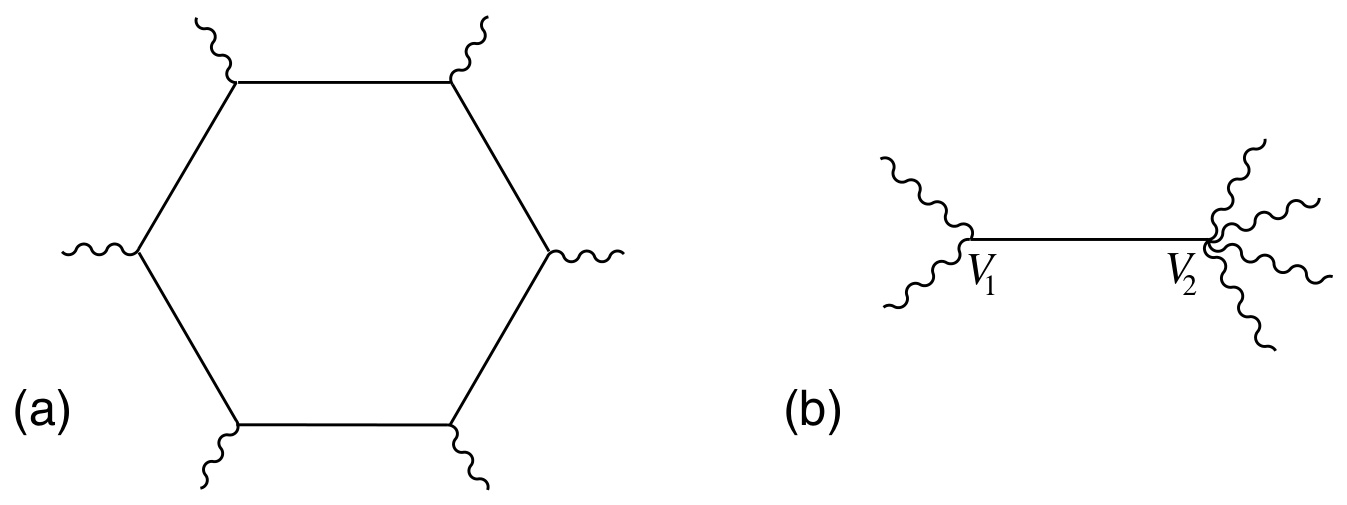
\includegraphics[width=0.7\textwidth]{figure/Fig12.1.jpg}
	\caption{Graphs contributing to the spacetime anomalies. One of the six external lines is a current and the others are gauge or gravitational fields: (a) 1-loop hexagon graph; (b) canceling tree graph from the exchange of the $B_{\mu\nu}$ field.}
	\label{fig:12.1}
\end{figure}

\begin{equation}
	\delta Z[A] = -\pi \int \dif^{2}z\:\lambda^{a}(z,\bar{z})
	\Bigl[\hat{k}_{L}\partial_{z}A_{\bar{z}}^{a}(z,\bar{z})+\hat{k}_{R}\partial_{\bar{z}}A_{z}^{a}(z,\bar{z})\Bigr]\:.
	\label{12.2.3}
\end{equation}
\begin{tcolorbox}[breakable]
	\begin{remark}
		\textbf{Conventions.} The notes do not define $Z[A]$ or the normalization of $\lambda^{a}$, so we fix them here.
		\begin{itemize}
			\item[(i)] Currents are normalized as in \eqref{11.5.1} and \eqref{11.5.7} with $d^{ab}=\delta^{ab}$ (the basis chosen below \eqref{11.5.13}): $j^{a}(z)j^{b}(0)\sim\hat k_{L}\delta^{ab}z^{-2}+\mi c^{abc}j^{c}(0)z^{-1}$, and likewise for $\tilde\jmath^{a}(\bar z)$ with $\hat k_{R}$. Since $d^{ab}=\delta^{ab}$, index positions on $c^{abc}$ do not matter, and $c^{abc}$ is totally antisymmetric.
			\item[(ii)] $Z[A]\equiv\bigl\langle\exp\bigl(\mi\int\dif^{2}z\,[A^{a}_{\bar z}j^{a}+A^{a}_{z}\tilde\jmath^{a}]\bigr)\bigr\rangle$, with $Z[0]=1$, and ``$\delta Z$'' means $\delta\ln Z$ (the same thing at leading order). Here $A_{\bar z}=A^{\text{can}}_{\bar z}/2\pi$, where $A^{\text{can}}$ couples to the canonically normalized Noether current $j/2\pi$ (Polchinski's normalization of CFT currents; this is the $2\pi$ of \eqref{12.3.33}). The factor $\mi$ is our choice: it is the Euclidean coupling of a real gauge field to Hermitian currents.
			\item[(iii)] $\delta A^{\text{can}}=D\lambda^{\text{can}}$ with $D=\partial-\mi[A^{\text{can}},\cdot\,]$, i.e.\ $\delta A^{\text{can},a}=\partial\lambda^{\text{can},a}+c^{abc}A^{\text{can},b}\lambda^{\text{can},c}$, as in \eqref{12.1.37} and \eqref{12.3.32}.
			\item[(iv)] The parameter in \eqref{12.2.3} is $\lambda\equiv\lambda^{\text{can}}/\pi$, so that $\delta A^{a}_{\bar z}=\frac12\partial_{\bar z}\lambda^{a}+\pi c^{abc}A^{b}_{\bar z}\lambda^{c}$. This is a choice: it is the normalization for which the coefficient is the printed $-\pi$. With $\lambda=\lambda^{\text{can}}/2\pi$ the same computation gives $-2\pi$.
			\item[(v)] $\dif^{2}z=2\dif\sigma^{1}\dif\sigma^{2}$ and $\partial_{\bar z}z^{-1}=2\pi\delta^{2}(z,\bar z)$, from \eqref{2.1.24}.
		\end{itemize}
		Write $\langle\mathcal O\rangle_{A}$ for the normalized expectation value in the presence of the background. The holomorphic half gives
		\begin{align*}
			\delta\ln Z&=\mi\int\dif^{2}z\,\delta A^{a}_{\bar z}\,\langle j^{a}(z)\rangle_{A}\\
			&\eqs{1} -\frac{\mi}{2}\int\dif^{2}z\,\lambda^{a}\langle\bar\partial j^{a}(z)\rangle_{A}+\mi\pi c^{abc}\int\dif^{2}z\,A^{b}_{\bar z}\lambda^{c}\langle j^{a}\rangle_{A},\\
			\langle\bar\partial j^{a}(z)\rangle_{A}&\eqs{2} \mi\int\dif^{2}w\,A^{b}_{\bar w}(w)\,\partial_{\bar z}\Bigl[\frac{\hat k_{L}\delta^{ab}}{(z-w)^{2}}+\frac{\mi c^{abc}\langle j^{c}(w)\rangle_{A}}{z-w}\Bigr]\\
			&\eqs{3} -2\pi\mi\hat k_{L}\,\partial_{z}A^{a}_{\bar z}(z)-2\pi c^{abc}A^{b}_{\bar z}(z)\langle j^{c}(z)\rangle_{A},\\
			\delta\ln Z&\eqs{4} -\pi\hat k_{L}\int\dif^{2}z\,\lambda^{a}\partial_{z}A^{a}_{\bar z}
			+\mi\pi\int\dif^{2}z\,\bigl(c^{abc}\lambda^{a}A^{b}_{\bar z}\langle j^{c}\rangle_{A}+c^{abc}A^{b}_{\bar z}\lambda^{c}\langle j^{a}\rangle_{A}\bigr)\\
			&\eqs{5} -\pi\hat k_{L}\int\dif^{2}z\,\lambda^{a}\partial_{z}A^{a}_{\bar z} .
		\end{align*}
		At (1), the $\frac12\partial_{\bar z}\lambda$ term was integrated by parts. At (2), $\bar\partial j^{a}=0$ away from other currents, so inside the correlator $\partial_{\bar z}$ acts only on the singular terms of the OPE \eqref{11.5.1} of $j^{a}(z)$ with the currents in the exponent. For currents that OPE is exact, so the result holds to all orders in $A$. At (3), $\partial_{\bar z}(z-w)^{-2}=-\partial_{z}\partial_{\bar z}(z-w)^{-1}=-2\pi\partial_{z}\delta^{2}(z-w)$ and $\partial_{\bar z}(z-w)^{-1}=2\pi\delta^{2}(z-w)$, after which the $w$ integral is trivial. At (4), $-\frac{\mi}{2}(-2\pi\mi)=-\pi$. At (5), relabeling $a\leftrightarrow c$ in the second term and using $c^{cba}=-c^{abc}$ shows that the two $c^{abc}$ terms cancel. This cancellation is the classical gauge invariance, and it is what ties the $\pi c^{abc}$ in (iv) to the factor $\mi$ in (ii). The antiholomorphic half is identical, with $\partial_{z}\bar z^{-1}=2\pi\delta^{2}$, and gives $-\pi\hat k_{R}\int\lambda^{a}\partial_{\bar z}A^{a}_{z}$. Together these give \eqref{12.2.3}.

		\emph{Counterterm and descent.} Split \eqref{12.2.3} as
		\begin{align*}
			&-\pi\int\lambda^{a}\bigl(\hat k_{L}\partial_{z}A^{a}_{\bar z}+\hat k_{R}\partial_{\bar z}A^{a}_{z}\bigr)\\
			&\quad=-\frac{\pi}{2}(\hat k_{L}-\hat k_{R})\int\lambda^{a}\bigl(\partial_{z}A^{a}_{\bar z}-\partial_{\bar z}A^{a}_{z}\bigr)
			-\frac{\pi}{2}(\hat k_{L}+\hat k_{R})\int\lambda^{a}\bigl(\partial_{z}A^{a}_{\bar z}+\partial_{\bar z}A^{a}_{z}\bigr),\\
			&\delta\int\dif^{2}z\,A^{a}_{z}A^{a}_{\bar z}\eqs{6} -\frac12\int\dif^{2}z\,\lambda^{a}\bigl(\partial_{z}A^{a}_{\bar z}+\partial_{\bar z}A^{a}_{z}\bigr) .
		\end{align*}
		At (6), the $c^{abc}$ terms cancel because $A^{a}_{z}A^{a}_{\bar z}$ is adjoint invariant. So the local counterterm $\ln Z\to\ln Z-\pi(\hat k_{L}+\hat k_{R})\int A^{a}_{z}A^{a}_{\bar z}$ removes the second piece. The first piece, $\propto(\hat k_{L}-\hat k_{R})$, cannot be removed and is the genuine anomaly: it vanishes for vector-like theories. It is the consistent anomaly obtained by descent from $I_{4}\propto\operatorname{Tr}(F\wedge F)$: by the box after \eqref{12.1.37}, $\dif\omega_{3}=\operatorname{Tr}(F\wedge F)$ and $\delta\omega_{3}=\dif\operatorname{Tr}(\lambda\dif A)$, so $\omega^{1}_{2}=\operatorname{Tr}(\lambda\dif A)$, and $\dif A=(\partial_{z}A_{\bar z}-\partial_{\bar z}A_{z})\dif z\wedge\dif\bar z$ reproduces the combination $\lambda^{a}(\partial_{z}A^{a}_{\bar z}-\partial_{\bar z}A^{a}_{z})$. Descent also explains why the anomaly is exactly linear in $A$. In the heterotic application below, $\hat k_{L}=1$ (the $\lambda^{A}$) and $\hat k_{R}=0$.
	\end{remark}
\end{tcolorbox}

\section{Superspace and Superfields}

To construct superstring perturbation theory, it is more beneficial to first give superconformal symmetry a more geometric interpretation. To do this, we need a \textit{supermanifold}, which is a world-sheet with one ordinary complex coordinate $z$ and one anticommuting complex coordinate $\theta$, where
\begin{equation}
	\theta^{2}=\bar{\theta}^{2} = \{\theta,\bar{\theta}\} = 0 \:. \label{12.3.1}
\end{equation}
Due to anticommutativity, the Taylor expansion of any function of $\theta$ and $\bar{\theta}$ is truncated. Thus, we can view any function on the supermanifold as a set of ordinary functions appearing in the Taylor expansion. However, just as the operator "$\int\theta$" has many properties of an ordinary integral and thus we call it an integration, the behavior of $\theta$ is also very much like a coordinate, so it is useful to view this as a manifold with both ordinary and anticommuting coordinates.

We can view ordinary conformal transformations this way. Under a generalized transformation $z^{\prime}(z,\bar{z})$ of world-sheet coordinates, the transformation of derivatives is
\begin{equation}
	\partial_{z} = \frac{\partial z^{\prime}}{\partial z} \partial_{z^{\prime}}
	+\frac{\partial \bar{z}^{\prime}}{\partial z} \partial_{\bar{z}^{\prime}} \:.\label{12.3.2}
\end{equation}
Conformal transformations are those transformations that turn $\partial_{z}$ into a multiple of itself.

Define \textit{superderivatives},
\begin{equation}
	D_{\theta} = \partial_{\theta} + \theta \partial_{z}\:, \qquad \quad 
	D_{\bar{\theta}} = \partial_{\bar{\theta}}+ \bar{\theta}\partial_{\bar{z}} \:, \label{12.3.3}
\end{equation}
which have the following properties
\begin{equation}
	D_{\theta}^{2} = \partial_{z}\:, \qquad D_{\bar{\theta}}^{2} = \partial_{\bar{z}}\:,\qquad
	\{D_{\theta},D_{\bar{\theta}}\} = 0 \:. \label{12.3.4}
\end{equation}
\begin{tcolorbox}[breakable]
	Note that
	\begin{align*}
		(\partial_{\theta}+\theta\partial_{z})^{2}f =\partial_{\theta}\Bigl(\theta \partial_{z}f\Bigr)
		+\theta \partial_{z}\partial_{\theta} f = \partial_{z}f - \theta \partial_{\theta}\partial_{z}f
		+\theta \partial_{z}\partial_{\theta} f \:,
	\end{align*}
	The absence of a quadratic term in the first equal sign is due to the anticommutativity of $\theta$, and the negative sign of the second term in the second equal sign is for the same reason.
	\begin{align*}
		\{D_{\theta},D_{\bar{\theta}}\} &=\partial_{\theta}\partial_{\bar{\theta}}f+ \theta\bar{\theta}\partial_{z}\partial_{\bar{z}}f+\theta\partial_{\bar{\theta}}\partial_{z}f
		-\bar{\theta}\partial_{\theta}\partial_{\bar{z}}f \\
		&\quad +\partial_{\bar{\theta}}\partial_{\theta}f+ \bar{\theta}\theta\partial_{z}\partial_{\bar{z}}f
		+\bar{\theta}\partial_{\theta}\partial_{\bar{z}}f -\theta\partial_{\bar{\theta}}\partial_{z}f =0
	\end{align*}
\end{tcolorbox}
\noindent Superconformal transformations $z^{\prime}(z,\theta)$, $\theta^{\prime}(z,\theta)$ are transformations that turn $D_{\theta}$ into a multiple of itself. From
\begin{equation}
	D_{\theta} = D_{\theta} \theta^{\prime} \partial_{\theta^{\prime}}
	+D_{\theta}z^{\prime}\partial_{z^{\prime}} + D_{\theta}\bar{\theta}^{\prime}\partial_{\bar{\theta}^{\prime}}
	+D_{\theta}\bar{z}^{\prime}\partial_{\bar{z}^{\prime}} \:, \label{12.3.5}
\end{equation}
it follows that superconformal transformations satisfy
\begin{equation}
	D_{\theta}\bar{\theta}^{\prime}=D_{\theta}\bar{z}^{\prime}=0\:, \qquad \quad
	D_{\theta}z^{\prime} = \theta^{\prime}D_{\theta}\theta^{\prime} \:, \label{12.3.6}
\end{equation}
hence
\begin{equation}
	D_{\theta}= (D_{\theta}\theta^{\prime})D_{\theta^{\prime}} \:. \label{12.3.7}
\end{equation}
\begin{tcolorbox}[breakable]
	First prove \eqref{12.3.5}
	\begin{align*}
		D_{\theta} = \frac{\partial}{\partial \theta} + \theta \frac{\partial}{\partial z}
		&= \frac{\partial \theta^{\prime}}{\partial \theta} \frac{\partial}{\partial \theta^{\prime}}
		+ \frac{\partial z^{\prime}}{\partial \theta} \frac{\partial}{\partial z^{\prime}} 
		+\frac{\partial \bar{\theta}^{\prime}}{\partial \theta} \frac{\partial}{\partial \bar{\theta^{\prime}}}
		+ \frac{\partial \bar{z}^{\prime}}{\partial \theta} \frac{\partial}{\partial \bar{z}^{\prime}} \\
		&\quad+ \theta \frac{\partial \theta^{\prime}}{\partial z}\frac{\partial}{\partial \theta^{\prime}}
		+\theta \frac{\partial z^{\prime}}{\partial z}\frac{\partial}{\partial z^{\prime}}
		+ \theta \frac{\partial \bar{\theta}^{\prime}}{\partial z}\frac{\partial}{\partial \bar{\theta}^{\prime}}
		+\theta \frac{\partial \bar{z}^{\prime}}{\partial z}\frac{\partial}{\partial \bar{z}^{\prime}} \\
		&=D_{\theta} \theta^{\prime} \partial_{\theta^{\prime}}
		+D_{\theta}z^{\prime}\partial_{z^{\prime}} + D_{\theta}\bar{\theta}^{\prime}\partial_{\bar{\theta}^{\prime}}
		+D_{\theta}\bar{z}^{\prime}\partial_{\bar{z}^{\prime}} ,
	\end{align*}
	Using \eqref{12.3.6} on \eqref{12.3.5} yields
	\begin{align*}
		D_{\theta} \theta^{\prime} \partial_{\theta^{\prime}}
		+D_{\theta}z^{\prime}\partial_{z^{\prime}} + D_{\theta}\bar{\theta}^{\prime}\partial_{\bar{\theta}^{\prime}}
		+D_{\theta}\bar{z}^{\prime}\partial_{\bar{z}^{\prime}}
		=D_{\theta} \theta^{\prime} \partial_{\theta^{\prime}}
		+\theta^{\prime}D_{\theta}\theta^{\prime}\partial_{z^{\prime}}=(D_{\theta}\theta^{\prime})D_{\theta^{\prime}}\:.
	\end{align*}
\end{tcolorbox}
\noindent Using $D_{\theta}^{2}=\partial_{z}$ allows concluding that
\begin{equation}
	\partial_{\bar{z}}z^{\prime}=\partial_{\bar{\theta}}z^{\prime}=\partial_{\bar{z}}\theta^{\prime}
	=\partial_{\bar{\theta}}\theta^{\prime} =0  \label{12.3.8}
\end{equation}
\begin{tcolorbox}[breakable]
	The conjugate of \eqref{12.3.6} states $D_{\bar\theta}\theta'=D_{\bar\theta}z'=0$. Applying $D_{\bar\theta}$ once more and using $D_{\bar\theta}^{2}=\partial_{\bar z}$ from \eqref{12.3.4},
	\begin{align*}
		\partial_{\bar z}z'\eqs{1} D_{\bar\theta}\bigl(D_{\bar\theta}z'\bigr)=0,\qquad
		\partial_{\bar\theta}z'\eqs{2} D_{\bar\theta}z'-\bar\theta\,\partial_{\bar z}z'=0 ,
	\end{align*}
	and identically for $\theta'$. At (1), $D_{\bar\theta}^{2}=\partial_{\bar z}$. At (2), the definition \eqref{12.3.3} of $D_{\bar\theta}$ was used together with the result of (1). So $z'$ and $\theta'$ depend on neither $\bar z$ nor $\bar\theta$.
\end{tcolorbox}
\noindent and its conjugate relations. From this, we can solve for superconformal transformations and represent them using a holomorphic commuting function $f(z)$ and a holomorphic anticommuting function $g(z)$,
\begin{subequations}
	\begin{align}
		z^{\prime}(z,\theta) &= f(z)+\theta g(z)h(z) \:, \qquad 
		\theta^{\prime}(z,\theta)=g(z)+\theta h(z) \:, \label{12.3.9a} \\
		h(z) &= \pm\Bigl[\partial_{z}f(z)+g(z)\partial_{z}g(z)\Bigr]^{1/2} \label{12.3.9b}
	\end{align} \label{12.3.9}
\end{subequations}
The infinitesimal form is
\begin{equation}
	\delta z= \epsilon[v(z)-\mi\theta\eta(z)] \:, \qquad 
	\delta \theta =\epsilon[-\mi\eta(z)+\tfrac{1}{2}\theta\partial v(z)]  \label{12.3.10}
\end{equation}
where $\epsilon$ and $v$ commute, and $\eta$ anticommutes. They satisfy the superconformal algebra \eqref{10.1.11}.
\begin{tcolorbox}[breakable]
	First, $z^{\prime}$ must be in the form shown in \eqref{12.3.9a}. We can write $\theta^{\prime}$ as
	\[
	\theta^{\prime}(z,\theta)=g^{\prime}(z)+\theta h^{\prime}(z)
	\]
	Then use \eqref{12.3.6}
	\begin{align*}
		D_{\theta}z^{\prime} &= (\partial_{\theta}+\theta\partial_{z})(f+\theta gh)= gh+\theta \partial_{z} f \\
		\theta^{\prime}D_{\theta}\theta^{\prime} &=(g^{\prime}+\theta h^{\prime})(\partial_{\theta}+\theta\partial_{z})
		(g^{\prime}+\theta h^{\prime})
		=(g^{\prime}+\theta h^{\prime})(h^{\prime}+\theta \partial_{z} g^{\prime}) \\
		&=g^{\prime}h^{\prime}+\theta (h^{\prime}h^{\prime}-g^{\prime}\partial_{z} g^{\prime})
	\end{align*}
	From this it is not difficult to obtain
	\[
	g^{\prime}h^{\prime}=gh \:, \qquad h^{\prime}h^{\prime}=g^{\prime}\partial_{z} g^{\prime}+\partial f 
	\]
	Choosing $g^{\prime}=g$ and $h^{\prime}=h$ is completely possible, thus obtaining \eqref{12.3.9}.
	
	For the infinitesimal form, it is easy to see that $f\sim O(z)$, $h\sim O(1)$ and $g\sim O(\epsilon)$, which means \eqref{12.3.9b} must take the positive sign; therefore, we might as well take $f=z+\epsilon v(z)$ and $g=-\mi\epsilon\eta(z)$, then \eqref{12.3.9b} yields $h$:
	\[
	h=1+\tfrac{1}{2}\epsilon\partial_{z}v(z) \:.
	\]
\end{tcolorbox}

Analogous to the transformation of conformal tensors, the transformation of a \textit{tensor superfield} with weight $(h,\tilde{h})$ is
\begin{equation}
	(D_{\theta}\theta^{\prime})^{2h}(D_{\bar{\theta}}\bar{\theta}^{\prime})^{2\tilde{h}}
	\bm{\phi}^{\prime}(\bm{z}^{\prime},\bar{\bm{z}}^{\prime}) = \bm{\phi}(\bm{z},\bar{\bm{z}}) \:, \label{12.3.11}
\end{equation}
where $\bm{z}$ represents $(z,\theta)$. In an infinitesimal superconformal transformation $\delta \theta=\epsilon\eta(z)$,
\begin{equation}
	\delta\bm{\phi}(\bm{z},\bar{\bm{z}})=-\epsilon
	\Bigl[2h\theta\partial\eta(z)+\eta(z)Q_{\theta}+2\tilde{h}\bar{\theta}\bar{\partial}\bar{\eta}(\bar{z})
	+\bar{\eta}(\bar{z})Q_{\bar{\theta}}\Bigr]\bm{\phi}(\bm{z},\bar{\bm{z}}) \:, \label{12.3.12}
\end{equation}
where $Q_{\theta}=\partial_{\theta}-\theta\partial_{z}$ and $Q_{\bar{\theta}}=\partial_{\bar{\theta}}-\bar{\theta}\partial_{\bar{z}}$.
\begin{tcolorbox}[breakable]
	$\delta\theta = \epsilon\eta(z)$ corresponds to taking $g(z)=\epsilon\eta(z),\,h(z)=1$ and $f(z)=z$ in \eqref{12.3.9a}, then $z^{\prime}=z+\epsilon\theta\eta(z)$, so $\delta \bm{\phi}$ is (considering only the holomorphic part for simplicity):
	\begin{align*}
		\delta\bm{\phi}&= \bm{\phi}^{\prime}(\bm{z})-\bm{\phi}(\bm{z}) = \bm{\phi}^{\prime}(z^{\prime}-\epsilon\theta\eta,\theta^{\prime}-\epsilon\eta)-\bm{\phi}(z,\theta) \\
		&=\bm{\phi}^{\prime}(z^{\prime},\theta^{\prime})
		-\epsilon\theta\eta\partial_{z^{\prime}}\bm{\phi}^{\prime}(z^{\prime},\theta^{\prime})
		-\epsilon\eta\partial_{\theta^{\prime}}\bm{\phi}^{\prime}(z^{\prime},\theta^{\prime}) -\bm{\phi}(z,\theta)\\
		&=(D_{\theta}\theta^{\prime})^{-2h}\bm{\phi}(\bm{z})-\bm{\phi}(\bm{z})
		-\epsilon\eta Q_{\theta}\Bigl((D_{\theta}\theta^{\prime})^{-2h}\bm{\phi}(\bm{z})\Bigr) \\
		&= -2h\epsilon\theta(\partial_{z}\eta) \bm{\phi} -\epsilon\eta Q_{\theta}\bm{\phi}
	\end{align*}
	Note that we used $(D_{\theta}\theta^{\prime})^{-2h}=(1+\epsilon\theta\partial\eta)^{-2h}=1-2h\epsilon\theta\partial\eta$, and in the third equal sign we used the anticommutativity of $\theta$ and $\eta$, thus obtaining $Q_{\theta}$ rather than $D_{\theta}$.
\end{tcolorbox}
Expanding into a Taylor series in $\theta$—focusing only on the holomorphic part for simplicity—we have
\begin{equation}
	\bm{\phi}(\bm{z}) = \mathcal{O}(z)+\theta \varPsi(z) \:. \label{12.3.13}
\end{equation}
Then the infinitesimal transformation \eqref{12.3.12} is
\begin{equation}
	\delta \mathcal{O} = -\epsilon\eta\varPsi\:, \qquad 
	\delta \varPsi=-\epsilon[2h\partial\eta \mathcal{O}+\eta\partial\mathcal{O}] \:. \label{12.3.14}
\end{equation}
Written as OPE coefficients \eqref{10.3.4}, this is
\begin{subequations}
	\begin{align}
		G_{{-}1/2}\cdot \mathcal{O} &= \varPsi\:, \qquad G_{r}\cdot \mathcal{O}=0\:, \quad r\geq \tfrac{1}{2} \:,\label{12.3.15a} \\ 
		G_{{-}1/2}\cdot \varPsi &= \partial\mathcal{O}\:, \qquad G_{1/2}\cdot \varPsi = 2h\mathcal{O}\:,
		\qquad G_{r}\cdot\varPsi=0\:,\quad r\geq \tfrac{3}{2} \:. \label{12.3.15b}
	\end{align}\label{12.3.15}
\end{subequations}
\begin{tcolorbox}[breakable]
	\begin{remark}
		Derivation of \eqref{12.3.14} and \eqref{12.3.15}. Insert $\bm\phi=\mathcal O+\theta\varPsi$ into \eqref{12.3.12} (holomorphic part; $\epsilon$ commuting, $\eta$ anticommuting):
		\begin{align*}
			\delta\mathcal O+\theta\,\delta\varPsi
			&=-\epsilon\Bigl[2h\theta\partial\eta+\eta\bigl(\partial_{\theta}-\theta\partial\bigr)\Bigr](\mathcal O+\theta\varPsi)
			\eqs{1} -\epsilon\Bigl[2h\theta\partial\eta\,\mathcal O+\eta\varPsi-\eta\theta\,\partial\mathcal O\Bigr]\\
			&\eqs{2} -\epsilon\eta\varPsi+\theta\Bigl(-\epsilon\bigl[2h\partial\eta\,\mathcal O+\eta\partial\mathcal O\bigr]\Bigr) .
		\end{align*}
		At (1), $\theta\partial\eta\,\theta\varPsi=-\theta\theta\,\partial\eta\varPsi=0$, $\partial_{\theta}(\theta\varPsi)=\varPsi$ and $\theta\partial(\theta\varPsi)=0$. At (2), $-\eta\theta=\theta\eta$. Reading off the $\theta^{0}$ and $\theta^{1}$ terms gives \eqref{12.3.14}.

		To get \eqref{12.3.15}, compare with the Ward identity \eqref{10.3.4}, $\delta\mathscr A=-\epsilon\sum_{n}\frac{1}{n!}\partial^{n}\eta\,G_{n-1/2}\cdot\mathscr A$, identifying its $\eta$ with the one in \eqref{12.3.12}. Since $\eta(z)$ is arbitrary, the coefficients of $\eta,\partial\eta,\partial^{2}\eta,\dots$ at the operator position must match separately:
		\begin{align*}
			\delta\mathcal O=-\epsilon\bigl[\eta\,G_{-1/2}+\partial\eta\,G_{1/2}+\cdots\bigr]\cdot\mathcal O\;&\overset{!}{=}\;-\epsilon\eta\varPsi ,\\
			\delta\varPsi=-\epsilon\bigl[\eta\,G_{-1/2}+\partial\eta\,G_{1/2}+\cdots\bigr]\cdot\varPsi\;&\overset{!}{=}\;-\epsilon\bigl[\eta\,\partial\mathcal O+\partial\eta\,2h\mathcal O\bigr] ,
		\end{align*}
		so that
		\begin{align*}
			G_{-1/2}\cdot\mathcal O=\varPsi,\quad G_{r\ge1/2}\cdot\mathcal O=0,\qquad
			G_{-1/2}\cdot\varPsi=\partial\mathcal O,\quad G_{1/2}\cdot\varPsi=2h\mathcal O,\quad G_{r\ge3/2}\cdot\varPsi=0 .
		\end{align*}
	\end{remark}
\end{tcolorbox}
Whether through the use of the NS algebra or by considering pure conformal transformations $\delta z=\epsilon v(z)$, it can be found that $\mathcal{O}$ is a tensor with weight $h$, while $\varPsi$ is a tensor with weight $h+\tfrac{1}{2}$, so both are annihilated by all Virasoro lowering generators. The lowest component $\mathcal{O}$ of this tensor superfield is a \textit{superconformal primary field}, which is annihilated by all lowering generators of the NS algebra.

Contrasting rigid translation, now rigid world-sheet supersymmetric translation is $\delta\theta ={-}\mi\epsilon\eta$, $\delta z={-}\mi\epsilon\theta\eta$. The Ward identity for $T_{F}$ gives the corresponding generator
\begin{equation}
	G_{{-}1/2}\cdot \sim -\mi Q_{\theta} = -\mi(\partial_{\theta}-\theta\partial_{z}) \label{12.3.16}
\end{equation}
\begin{tcolorbox}[breakable]
	\begin{remark}
		\textbf{Conventions, and the inconsistency.} The text uses two incompatible identifications of the parameter $\eta$ with a superspace transformation. \eqref{12.3.12}--\eqref{12.3.15} take $\delta\theta=+\epsilon\eta$, while \eqref{12.3.10} and \eqref{12.3.16} take $\delta\theta=-\mi\epsilon\eta$, so their $\eta$'s differ by a factor $\mi$. Neither matches the free-field OPE: with \eqref{12.3.19}, $G_{-1/2}\cdot X=-\mi\psi=-\varPsi$, whereas \eqref{12.3.15} says $+\varPsi$, and $-\mi Q_{\theta}\bm X|_{\theta=0}=-\mi\varPsi=+\psi$. In addition, \eqref{10.3.4} is printed with $-\epsilon$, while the Ward identity actually used to derive \eqref{10.1.10a}--\eqref{10.1.10c} (the box before it) gives $+\mi\epsilon$. We fix one consistent set:
		\begin{itemize}
			\item[(i)] The Ward identity of the box before \eqref{10.1.10a} (Polchinski's \eqref{2.3.11} form): $\delta\mathscr A(z)=\mi\epsilon\operatorname{Res}_{w\to z}\eta(w)T_{F}(w)\mathscr A(z)$. With $T_{F}(w)\mathscr A(z)=\sum_{r}(w-z)^{-r-3/2}G_{r}\cdot\mathscr A(z)$ this is $\delta\mathscr A=\mi\epsilon\sum_{n}\frac{1}{n!}\partial^{n}\eta\,G_{n-1/2}\cdot\mathscr A$, i.e.\ \eqref{10.3.4} with $-\epsilon\to\mi\epsilon$.
			\item[(ii)] $T_{F}=\mi(2/\alpha')^{1/2}\psi\cdot\partial X$ at $\alpha'=2$, the superfield \eqref{12.3.19}, and $\psi\psi\sim\eta/z$, $XX\sim-\ln\lvert z\rvert^{2}$.
			\item[(iii)] $G_{r}$ is fermionic: $G_{r}\cdot(\theta\mathscr A)=-\theta\,G_{r}\cdot\mathscr A$.
		\end{itemize}
		The OPE coefficients $G_{r}\cdot$ are fixed by $T_{F}$ alone and do not depend on (i). Only the map from $\eta$ to $(\delta z,\delta\theta)$ does.

		\emph{The generator on the free superfield.} From the OPEs in the box before \eqref{10.1.10a}, at $\alpha'=2$,
		\begin{gather*}
			T_{F}(w)X^{\mu}(z)\sim\frac{-\mi\psi^{\mu}(z)}{w-z},\quad T_{F}(w)\psi^{\mu}(z)\sim\frac{\mi\partial X^{\mu}(z)}{w-z}\\
			\Longrightarrow\quad G_{-1/2}\cdot X^{\mu}=-\mi\psi^{\mu},\quad G_{-1/2}\cdot\psi^{\mu}=\mi\partial X^{\mu},
		\end{gather*}
		\begin{align*}
			G_{-1/2}\cdot\bm X^{\mu}=G_{-1/2}\cdot X^{\mu}+\mi\,G_{-1/2}\cdot(\theta\psi^{\mu})
			&\eqs{1} -\mi\psi^{\mu}-\mi\theta\,(\mi\partial X^{\mu})=-\mi\psi^{\mu}+\theta\partial X^{\mu}\\
			&\eqs{2} -Q_{\theta}\bm X^{\mu} .
		\end{align*}
		At (1), (iii) was used. At (2), $Q_{\theta}\bm X=\partial_{\theta}\bm X-\theta\partial\bm X=\mi\psi-\theta\partial X$ (holomorphic part). As a check, $G_{-1/2}\cdot(G_{-1/2}\cdot X)=-\mi\,G_{-1/2}\cdot\psi=\partial X=L_{-1}\cdot X$, as required by $\{G_{-1/2},G_{-1/2}\}=2L_{-1}$.

		\emph{The transformation generated by $\eta$.} By (i), $\delta X=\mi\epsilon\eta(-\mi\psi)=\epsilon\eta\psi$ and $\delta\psi=\mi\epsilon\eta(\mi\partial X)=-\epsilon\eta\partial X$, which is \eqref{10.1.10a}--\eqref{10.1.10c} at $\alpha'=2$. The superspace map $\delta\theta=a\epsilon\eta$, $\delta z=a\epsilon\theta\eta$ gives, by the box after \eqref{12.3.12} with $\eta\to a\eta$ (constant $\eta$, $h=0$),
		\begin{align*}
			\delta\bm X=-a\epsilon\eta\,Q_{\theta}\bm X
			\quad\Longrightarrow\quad \delta X=-\mi a\,\epsilon\eta\psi
			\quad\eqs{3}\quad a=\mi .
		\end{align*}
		At (3), this was matched to $\delta X=\epsilon\eta\psi$. So $\eta$ generates $\delta\theta=\mi\epsilon\eta$, $\delta z=\mi\epsilon\theta\eta$, which is \eqref{12.3.10} with $\eta\to-\eta$.

		\emph{General tensor superfield.} For weight $h$, the transformation with $\delta\theta=\mi\epsilon\eta(z)$ is \eqref{12.3.12} with $\eta\to\mi\eta$, so by the box after \eqref{12.3.15}, $\delta\mathcal O=-\mi\epsilon\eta\varPsi$ and $\delta\varPsi=-\mi\epsilon(2h\partial\eta\,\mathcal O+\eta\partial\mathcal O)$. Matching with (i) coefficient by coefficient in $\eta,\partial\eta,\dots$:
		\begin{align*}
			G_{-1/2}\cdot\mathcal O=-\varPsi,\quad G_{r\ge1/2}\cdot\mathcal O=0,\\
			G_{-1/2}\cdot\varPsi=-\partial\mathcal O,\quad G_{1/2}\cdot\varPsi=-2h\,\mathcal O,\quad G_{r\ge3/2}\cdot\varPsi=0,
		\end{align*}
		and for Grassmann-even $\mathcal O$,
		\begin{align*}
			G_{-1/2}\cdot\bm\phi=G_{-1/2}\cdot\mathcal O-\theta\,G_{-1/2}\cdot\varPsi\eqs{4} -\varPsi+\theta\partial\mathcal O=-Q_{\theta}\bm\phi .
		\end{align*}
		At (4), the component results above were used. This agrees with the free-field result ($h=0$, $\mathcal O=X$, $\varPsi=\mi\psi$).

		So in one consistent convention, \eqref{12.3.16} reads $G_{-1/2}\cdot\sim-Q_{\theta}$, and \eqref{12.3.15} holds with $\varPsi\to-\varPsi$ (i.e.\ for the superfield written as $\mathcal O-\theta\varPsi$). The structural statement, that $G_{-1/2}\cdot$ acts on superfields as $Q_{\theta}$ up to a constant phase and thus generates the rigid translation $\theta\to\theta+{}$const, $z\to z+\theta\,{}$const, holds in any convention. The phase is what (i)--(iii) fix. Acting twice gives $L_{-1}$, as checked on $X$ above.
	\end{remark}
\end{tcolorbox}
This generalizes $L_{{-}1}\cdot \sim \partial_{z}$ obtained in CFT.

\subsection*{Actions and backgrounds}

The super-Jacobian matrix of transformation \eqref{12.3.9} is
\begin{equation}
	\dif z^{\prime}\,\dif\theta^{\prime} = \dif z\,\dif\theta\,D_{\theta}\theta^{\prime}\:. \label{12.3.17}
\end{equation}
\begin{tcolorbox}[breakable]
	\begin{remark}
		Derivation of \eqref{12.3.17}. The Jacobian of a change of variables $(z,\theta)\to(z',\theta')$ is the Berezinian (superdeterminant)
		\[
		\dif z'\,\dif\theta'=\dif z\,\dif\theta\;\frac{A-BD^{-1}C}{D},\qquad
		A=\partial_{z}z',\quad B=z'\overleftarrow{\partial_{\theta}},\quad C=\partial_{z}\theta',\quad D=\partial_{\theta}\theta' .
		\]
		The fermionic derivative in the odd entry $B$ must act from the right; with it, $\int\dif z'\dif\theta'\,F=\int\dif z\,\dif\theta\,\mathrm{Ber}\,F$. This can be checked directly on $z'=z+\theta g$, $\theta'=\theta+g$, for which both sides give $\mathrm{Ber}=1+gg'+\theta g'$. For \eqref{12.3.9}, $z'=f+\theta gh=f-gh\,\theta$, so
		\begin{align*}
			A&=\partial f+\theta\,\partial(gh),\qquad B=-gh,\qquad C=\partial g+\theta\,\partial h,\qquad D=h,\\
			A-BD^{-1}C&\eqs{1} \partial f+\theta(\partial g\,h+g\,\partial h)+g\,\partial g+g\theta\,\partial h
			\eqs{2} \partial f+g\,\partial g+\theta\,h\,\partial g
			\eqs{3} h^{2}+\theta\,h\,\partial g ,\\
			\frac{A-BD^{-1}C}{D}&=h+\theta\,\partial g
			\eqs{4} D_{\theta}\theta' .
		\end{align*}
		At (1), $-BD^{-1}C=g(\partial g+\theta\partial h)$. At (2), $g\theta=-\theta g$, so the two $\theta g\,\partial h$ terms cancel. At (3), $h^{2}=\partial f+g\partial g$ from \eqref{12.3.9b}. At (4), $D_{\theta}\theta'=(\partial_{\theta}+\theta\partial)(g+\theta h)=h+\theta\partial g$.
	\end{remark}
\end{tcolorbox}
To construct a superconformally invariant action, the Lagrangian density must be a tensor superfield with weight $(\tfrac{1}{2},\tfrac{1}{2})$. The product of two tensor superfields is also a tensor superfield, whose weight is the sum of the original two weights, $(h,\tilde{h})=(h_{1},\tilde{h}_{1})+(h_{2},\tilde{h}_{2})$. Additionally, the superderivative $D_{\theta}$ turns a $(0,\tilde{h})$ tensor superfield into a $(\tfrac{1}{2},\tilde{h})$ tensor superfield, while $D_{\bar{\theta}}$ turns an $(h,0)$ tensor superfield into an $(h,\tfrac{1}{2})$ tensor superfield.

We can construct an invariant action from $d$ tensors $\bm{X}^{\mu}(\bm{z},\bar{\bm{z}})$ with weight $(0,0)$:
\begin{equation}
	S= \frac{1}{4\pi} \int \dif^{2}z\,\dif^{2}\theta\: D_{\bar{\theta}}\bm{X}^{\mu}D_{\theta}\bm{X}_{\mu}\:.\label{12.3.18} 
\end{equation}
The Taylor expansion of $\bm{X}^{\mu}$ with respect to $\theta$ is
\begin{equation}
	\bm{X}^{\mu}(\bm{z},\bar{\bm{z}})=X^{\mu}+\mi\theta \psi^{\mu}+\mi\bar{\theta}\tilde{\psi}^{\mu}
	+\theta\bar{\theta}F^{\mu} \:. \label{12.3.19}
\end{equation}
where $\alpha^{\prime}=2$ is set, and can be restored via $X^{\mu}\to X^{\mu}(2/\alpha^{\prime})^{1/2}$. Integration over $\dif^{2}\theta=\dif\theta\,\dif\bar{\theta}$ in the action picks out the coefficient of $\bar{\theta}\theta$
\begin{equation}
	S=\frac{1}{4\pi}\int\dif^{2}z\:\Bigl(\partial_{\bar{z}}X^{\mu}\partial_{z}X_{\mu}+\psi^{\mu}\partial_{\bar{z}}psi_{\mu}+\tilde{\psi}^{\mu}\partial_{z}\tilde{\psi}_{\mu}+F^{\mu}F_{\mu}\Bigr) \:. \label{12.3.20}
\end{equation}
The field $F^{\mu}$ is an auxiliary field, completely determined by the equations of motion—here being zero. The remainder of the action is identical to the previous \eqref{10.1.5}.

Many previous results can be recast in superfield form; the equation of motion is
\begin{equation}
	D_{\theta}D_{\bar{\theta}}\bm{X}^{\mu}(\bm{z},\bar{\bm{z}})=0\:. \label{12.3.21}
\end{equation}
\begin{tcolorbox}[breakable]
	\begin{remark}
		Derivation of \eqref{12.3.20} and \eqref{12.3.21}. Acting on \eqref{12.3.19} with \eqref{12.3.3},
		\begin{align*}
			D_{\theta}\bm X^{\mu}&\eqs{1} \mi\psi^{\mu}+\bar\theta F^{\mu}+\theta\partial X^{\mu}+\mi\theta\bar\theta\,\partial\tilde\psi^{\mu},\\
			D_{\bar\theta}\bm X^{\mu}&\eqs{1} \mi\tilde\psi^{\mu}-\theta F^{\mu}+\bar\theta\bar\partial X^{\mu}+\mi\bar\theta\theta\,\bar\partial\psi^{\mu} .
		\end{align*}
		At (1), $\partial_{\theta}(\theta\bar\theta F)=\bar\theta F$ and $\partial_{\bar\theta}(\theta\bar\theta F)=-\theta F$, and the $\theta\partial$ ($\bar\theta\bar\partial$) term keeps only the $\theta$-independent ($\bar\theta$-independent) components. In the product $D_{\bar\theta}\bm X^{\mu}D_{\theta}\bm X_{\mu}$, the $\bar\theta\theta$ component receives four contributions:
		\begin{align*}
			(\mi\tilde\psi^{\mu})(\mi\theta\bar\theta\,\partial\tilde\psi_{\mu})&\eqs{2}\bar\theta\theta\,\tilde\psi^{\mu}\partial\tilde\psi_{\mu},\qquad
			(-\theta F^{\mu})(\bar\theta F_{\mu})\eqs{2}\bar\theta\theta\,F^{\mu}F_{\mu},\\
			(\bar\theta\bar\partial X^{\mu})(\theta\partial X_{\mu})&=\bar\theta\theta\,\bar\partial X^{\mu}\partial X_{\mu},\qquad
			(\mi\bar\theta\theta\,\bar\partial\psi^{\mu})(\mi\psi_{\mu})\eqs{3}\bar\theta\theta\,\psi^{\mu}\bar\partial\psi_{\mu} .
		\end{align*}
		At (2), $\theta\bar\theta=-\bar\theta\theta$. At (3), $-\bar\partial\psi^{\mu}\psi_{\mu}=\psi_{\mu}\bar\partial\psi^{\mu}$ by anticommutation. Every other product has an unpaired $\theta$ or $\bar\theta$, or contains $\theta^{2}$ or $\bar\theta^{2}$. Since $\int\dif\theta\,\dif\bar\theta\,\bar\theta\theta=1$, this gives \eqref{12.3.20}, and the $F^{\mu}$ equation of motion is $F^{\mu}=0$. Similarly,
		\begin{align*}
			D_{\theta}D_{\bar\theta}\bm X^{\mu}
			\eqs{4} -F^{\mu}-\mi\bar\theta\,\bar\partial\psi^{\mu}+\mi\theta\,\partial\tilde\psi^{\mu}+\theta\bar\theta\,\partial\bar\partial X^{\mu}=0 .
		\end{align*}
		At (4), $\partial_{\theta}(\bar\theta\theta)=-\bar\theta$. The four components are $F^{\mu}=0$, $\bar\partial\psi^{\mu}=0$, $\partial\tilde\psi^{\mu}=0$ and $\partial\bar\partial X^{\mu}=0$, all the component equations of motion at once.
	\end{remark}
\end{tcolorbox}
For OPEs, invariance under translation and rigid supersymmetric transformations tells us it can only be a function of $z_{1}-z_{2}-\theta_{1}\theta_{2}$, $\theta_{1}-\theta_{2}$, and their conjugates. In this case,
\begin{equation}
	\bm{X}^{\mu}(\bm{z}_{1},\bar{\bm{z}}_{1})\bm{X}^{\nu}(\bm{z}_{2},\bar{\bm{z}}_{2})\sim
	-\eta^{\mu\nu}\ln\lvert z_{1}-z_{2}-\theta_{1}\theta_{2}\rvert^{2} \:, \label{12.3.22}
\end{equation}
which can be proven by expansion into component fields.
\begin{tcolorbox}[breakable]
	Translation and rigid supersymmetry transformations of $\theta$ tell us $z$ and $\theta$ can only appear as $z_{1}-z_{2}$ and $\theta_{1}-\theta_{2}$. Then rigid supersymmetry transformation of $z$ yields
	\[
	\delta_{\text{super}}(z_{1}-z_{2}) = -\mi\epsilon\theta_{1}\eta+\mi\epsilon\theta_{2}\eta \:,
	\]
	while rigid supersymmetry transformation of $\theta_{1}\theta_{2}$ yields
	\[
	\delta_{\text{super}}(\theta_{1}\theta_{2})= \delta(\theta_{1})\theta_{2}+\theta_{1}\delta(\theta_{2})
	=\theta_{1}(-\mi\epsilon\eta)+(-\mi\epsilon\eta)\theta_{2}
	\]
	The two cancel exactly.
\end{tcolorbox}
\begin{tcolorbox}[breakable]
	Component check of \eqref{12.3.22}. Expand in the nilpotent $\theta_{1}\theta_{2}$:
	\begin{align*}
		-\eta^{\mu\nu}\ln\lvert z_{12}-\theta_{1}\theta_{2}\rvert^{2}
		&\eqs{1} -\eta^{\mu\nu}\ln\lvert z_{12}\rvert^{2}+\eta^{\mu\nu}\frac{\theta_{1}\theta_{2}}{z_{12}}+\eta^{\mu\nu}\frac{\bar\theta_{1}\bar\theta_{2}}{\bar z_{12}} ,\\
		\bm X^{\mu}(\bm z_{1})\bm X^{\nu}(\bm z_{2})
		&\eqs{2} X^{\mu}X^{\nu}+\theta_{1}\theta_{2}\,\psi^{\mu}(z_{1})\psi^{\nu}(z_{2})+\bar\theta_{1}\bar\theta_{2}\,\tilde\psi^{\mu}(\bar z_{1})\tilde\psi^{\nu}(\bar z_{2})+\cdots .
	\end{align*}
	At (1), $\ln(z_{12}-\theta_{1}\theta_{2})=\ln z_{12}-\theta_{1}\theta_{2}/z_{12}$ exactly, since $(\theta_{1}\theta_{2})^{2}=0$. At (2), $(\mi\theta_{1}\psi^{\mu})(\mi\theta_{2}\psi^{\nu})=-\theta_{1}\psi^{\mu}\theta_{2}\psi^{\nu}=\theta_{1}\theta_{2}\psi^{\mu}\psi^{\nu}$; the dots are mixed $\psi\tilde\psi$ terms, which have no singular OPE, and terms with $F$, whose OPE is a contact term only. Matching coefficients reproduces $X^{\mu}X^{\nu}\sim-\eta^{\mu\nu}\ln\lvert z_{12}\rvert^{2}$, $\psi^{\mu}\psi^{\nu}\sim\eta^{\mu\nu}/z_{12}$ and $\tilde\psi^{\mu}\tilde\psi^{\nu}\sim\eta^{\mu\nu}/\bar z_{12}$, the free OPEs at $\alpha'=2$.
\end{tcolorbox}
The superconformal ghost action is built with tensor superfields $B$ and $C$ with weights $(\lambda-\frac{1}{2})$ and $(1-\lambda,0)$, respectively,
\begin{equation}
	S_{BC}=\frac{1}{2\pi}\int \dif^{2}z\,\dif^{2}\theta\: B D_{\bar{\theta}}C \:. \label{12.3.23}
\end{equation}
The equations of motion are
\begin{equation}
	D_{\bar{\theta}}B= D_{\bar{\theta}}C=0 \:. \label{12.3.24}
\end{equation}
Applying $D_{\bar{\theta}}$ to this equation yields $\partial_{\bar{z}}B=\partial_{\bar{z}}C=0$, and hence $\partial_{\bar{\theta}}B=\partial_{\bar{\theta}}C=0$. Thus the equations of motion yield
\begin{equation}
	B(\bm{z})=\beta(z)+\theta b(z) \:, \qquad C(\bm{z})=c(z)+\theta\gamma(z)\:. \label{12.3.25}
\end{equation}
This is identical to theory \eqref{10.1.17}. The OPE is
\begin{equation}
	B(\bm{z}_{1})C(\bm{z}_{2})\sim \frac{\theta_{1}-\theta_{2}}{z_{1}-z_{2}-\theta_{1}\theta_{2}}
	=\frac{\theta_{1}-\theta_{2}}{z_{1}-z_{2}} \:. \label{12.3.26}
\end{equation}
\begin{tcolorbox}[breakable]
	Components of \eqref{12.3.26}. The second equality holds because $(\theta_{1}-\theta_{2})\theta_{1}\theta_{2}=0$, so $\frac{\theta_{12}}{z_{12}-\theta_{1}\theta_{2}}=\frac{\theta_{12}}{z_{12}}\bigl(1+\frac{\theta_{1}\theta_{2}}{z_{12}}\bigr)=\frac{\theta_{12}}{z_{12}}$. With \eqref{12.3.25},
	\begin{align*}
		B(\bm z_{1})C(\bm z_{2})
		\eqs{1} \beta(z_{1})c(z_{2})+\theta_{1}\,b(z_{1})c(z_{2})+\theta_{2}\,\beta(z_{1})\gamma(z_{2})-\theta_{1}\theta_{2}\,b(z_{1})\gamma(z_{2})
		\sim\frac{\theta_{1}}{z_{12}}-\frac{\theta_{2}}{z_{12}} .
	\end{align*}
	At (1), $\beta$ is commuting and $b$ anticommutes with $\theta_{2}$. Matching powers of $\theta$ gives $b(z_{1})c(z_{2})\sim1/z_{12}$ and $\beta(z_{1})\gamma(z_{2})\sim-1/z_{12}$, which are the $bc$ and $\beta\gamma$ OPEs of chapter 10, with no singular $\beta c$ and $b\gamma$ terms.
\end{tcolorbox}
The superfield form makes writing the non-linear $\sigma$ model action very simple
\begin{align}
	S &= \frac{1}{4\pi}\int\dif^{2}z\,\dif^{2}\theta\:[G_{\mu\nu}(\bm{X})+B_{\mu\nu}(\bm{X})]
	D_{\bar{\theta}}\bm{X}^{\nu}D_{\theta}\bm{X}^{\mu} \nonumber \\ 
	&=\frac{1}{4\pi}\int \dif^{2}z\:\Bigl\{[G_{\mu\nu}(X)+B_{\mu\nu}(X)]\partial_{z}X^{\mu}\partial_{\bar{z}}X^{\nu}
	\nonumber \\
	&\qquad \quad+G_{\mu\nu}(X)(\psi^{\mu}\mathscr{D}_{\bar{z}}\psi^{\nu}+\tilde{\psi}^{\mu}\mathscr{D}_{z}\tilde{\psi}^{\nu})+\tfrac{1}{2}R_{\mu\nu\rho\sigma}(X)\psi^{\mu}\psi^{\nu}\tilde{\psi}^{\rho}\tilde{\psi}^{\sigma}\Bigr\}\:,
	\label{12.3.27}
\end{align}
auxiliary fields are eliminated in the second equal sign. The Christoffel connection and antisymmetric tensor field strength form the covariant derivative
\begin{subequations}
	\begin{align}
		\mathscr{D}_{\bar{z}}\psi^{\nu} &= \partial_{\bar{z}}\psi^{\nu}
		+\Bigl[\Gamma\indices{^\nu_\rho_\sigma}(X)+\tfrac{1}{2}H\indices{^\nu_\rho_\sigma}(X)\Bigr]\partial_{\bar{z}}X^{\rho}\psi^{\sigma} \:, \label{12.3.28a} \\
		\mathscr{D}_{z}\tilde{\psi}^{\nu} &= \partial_{z}\tilde{\psi}^{\nu} 
		+\Bigl[\Gamma\indices{^\nu_\rho_\sigma}(X)-\tfrac{1}{2}H\indices{^\nu_\rho_\sigma}(X)\Bigr]
		\partial_{z}X^{\rho}\tilde{\psi}^{\sigma} \:. \label{12.3.28b}
	\end{align} \label{12.3.28}
\end{subequations}
\begin{tcolorbox}[breakable]
	\begin{remark}
		Derivation of \eqref{12.3.27} and \eqref{12.3.28}. Write $E_{\mu\nu}=G_{\mu\nu}+B_{\mu\nu}$ and expand $E_{\mu\nu}(\bm X)$ around $X$ with $\bm X-X=\mi\theta\psi+\mi\bar\theta\tilde\psi+\theta\bar\theta F$:
		\begin{align*}
			E_{\mu\nu}(\bm X)&\eqs{1} E_{\mu\nu}+\mi\theta E_{\mu\nu,\rho}\psi^{\rho}+\mi\bar\theta E_{\mu\nu,\rho}\tilde\psi^{\rho}
			-\bar\theta\theta\bigl(E_{\mu\nu,\rho}F^{\rho}+E_{\mu\nu,\rho\sigma}\psi^{\rho}\tilde\psi^{\sigma}\bigr) .
		\end{align*}
		At (1), the quadratic term is $\frac12E_{,\rho\sigma}\bigl[(\mi\theta\psi^{\rho})(\mi\bar\theta\tilde\psi^{\sigma})+(\mi\bar\theta\tilde\psi^{\rho})(\mi\theta\psi^{\sigma})\bigr]=\theta\bar\theta\,E_{,\rho\sigma}\psi^{\rho}\tilde\psi^{\sigma}$, and $\theta\bar\theta=-\bar\theta\theta$. Using the components of $D_{\theta}\bm X$, $D_{\bar\theta}\bm X$ from the box after \eqref{12.3.21}, write $P^{\nu\mu}=D_{\bar\theta}\bm X^{\nu}D_{\theta}\bm X^{\mu}=P_{0}+\theta P_{\theta}+\bar\theta P_{\bar\theta}+\bar\theta\theta P_{\bar\theta\theta}$ with
		\begin{align*}
			P_{0}&=-\tilde\psi^{\nu}\psi^{\mu},\qquad
			P_{\theta}=-\mi F^{\nu}\psi^{\mu}-\mi\tilde\psi^{\nu}\partial X^{\mu},\qquad
			P_{\bar\theta}=\mi\bar\partial X^{\nu}\psi^{\mu}-\mi\tilde\psi^{\nu}F^{\mu},\\
			P_{\bar\theta\theta}&=\tilde\psi^{\nu}\partial\tilde\psi^{\mu}+F^{\nu}F^{\mu}+\bar\partial X^{\nu}\partial X^{\mu}-\bar\partial\psi^{\nu}\psi^{\mu} .
		\end{align*}
		The $\bar\theta\theta$ component of $E_{\mu\nu}(\bm X)P^{\nu\mu}$, picked out by $\int\dif^{2}\theta$, is then
		\begin{align*}
			\mathcal L&\eqs{2} E_{\mu\nu}P_{\bar\theta\theta}+E_{\bar\theta\theta}P_{0}+E_{\theta}P_{\bar\theta}-E_{\bar\theta}P_{\theta}\\
			&= E_{\mu\nu}\bigl(\partial X^{\mu}\bar\partial X^{\nu}+\psi^{\mu}\bar\partial\psi^{\nu}+\tilde\psi^{\nu}\partial\tilde\psi^{\mu}+F^{\nu}F^{\mu}\bigr)
			+E_{\mu\nu,\rho\sigma}\psi^{\rho}\tilde\psi^{\sigma}\tilde\psi^{\nu}\psi^{\mu}\\
			&\quad -E_{\mu\nu,\rho}\psi^{\rho}\psi^{\mu}\bar\partial X^{\nu}-E_{\mu\nu,\rho}\tilde\psi^{\rho}\tilde\psi^{\nu}\partial X^{\mu}+F^{\lambda}J_{\lambda} ,\\
			J_{\lambda}&\eqs{3} \bigl(E_{\mu\nu,\lambda}-E_{\lambda\nu,\mu}-E_{\mu\lambda,\nu}\bigr)\tilde\psi^{\nu}\psi^{\mu}
			\eqs{4} \bigl(-2\Gamma_{\lambda\mu\nu}+H_{\lambda\mu\nu}\bigr)\tilde\psi^{\nu}\psi^{\mu} .
		\end{align*}
		At (2), $(\theta E_{\theta})(\bar\theta P_{\bar\theta})=\bar\theta\theta E_{\theta}P_{\bar\theta}$ and $(\bar\theta E_{\bar\theta})(\theta P_{\theta})=-\bar\theta\theta E_{\bar\theta}P_{\theta}$, since $E_{\theta}$ and $E_{\bar\theta}$ are odd. At (3), the three terms linear in $F$ were collected and all fermion pairs ordered as $\tilde\psi\psi$. At (4), $\Gamma_{\lambda\mu\nu}=\frac12(G_{\lambda\mu,\nu}+G_{\lambda\nu,\mu}-G_{\mu\nu,\lambda})$ and $H_{\lambda\mu\nu}=\partial_{\lambda}B_{\mu\nu}+\partial_{\mu}B_{\nu\lambda}+\partial_{\nu}B_{\lambda\mu}$.

		\emph{Connection terms.} In the fermion kinetic terms the $B$ part is not zero but a total derivative plus a connection term:
		\[
		B_{\mu\nu}\psi^{\mu}\bar\partial\psi^{\nu}\simeq-\tfrac12B_{\mu\nu,\rho}\bar\partial X^{\rho}\psi^{\mu}\psi^{\nu},\qquad
		B_{\mu\nu}\tilde\psi^{\nu}\partial\tilde\psi^{\mu}\simeq\tfrac12B_{\mu\nu,\rho}\partial X^{\rho}\tilde\psi^{\mu}\tilde\psi^{\nu},
		\]
		obtained from $\bar\partial(B_{\mu\nu}\psi^{\mu}\psi^{\nu})$ and $\partial(B_{\mu\nu}\tilde\psi^{\nu}\tilde\psi^{\mu})$. Relabel so that every term reads $(\cdots)_{\mu\rho\sigma}\psi^{\mu}\psi^{\sigma}\bar\partial X^{\rho}$ and antisymmetrize in $\mu\sigma$:
		\begin{align*}
			&-E_{\mu\nu,\rho}\psi^{\rho}\psi^{\mu}\bar\partial X^{\nu}-\tfrac12B_{\mu\sigma,\rho}\psi^{\mu}\psi^{\sigma}\bar\partial X^{\rho}\\
			&\eqs{5} \Bigl[\tfrac12\bigl(G_{\mu\rho,\sigma}-G_{\sigma\rho,\mu}\bigr)-\tfrac12\bigl(B_{\sigma\rho,\mu}+B_{\rho\mu,\sigma}+B_{\mu\sigma,\rho}\bigr)\Bigr]\psi^{\mu}\psi^{\sigma}\bar\partial X^{\rho}\\
			&\eqs{6} \Bigl(\Gamma_{\mu\rho\sigma}+\tfrac12H_{\mu\rho\sigma}\Bigr)\psi^{\mu}\psi^{\sigma}\bar\partial X^{\rho}\\
			&=G_{\mu\nu}\psi^{\mu}\Bigl(\Gamma\indices{^\nu_\rho_\sigma}+\tfrac12H\indices{^\nu_\rho_\sigma}\Bigr)\bar\partial X^{\rho}\psi^{\sigma} .
		\end{align*}
		At (5), only the part antisymmetric in $\mu\sigma$ survives against $\psi^{\mu}\psi^{\sigma}$. At (6), $\Gamma_{\mu\rho\sigma}-\Gamma_{\sigma\rho\mu}=G_{\mu\rho,\sigma}-G_{\sigma\rho,\mu}$ (the symmetric part of $\Gamma_{\mu\rho\sigma}$ in $\mu\sigma$ drops), and the $B$ bracket is $H_{\mu\sigma\rho}=-H_{\mu\rho\sigma}$. Together with $G_{\mu\nu}\psi^{\mu}\bar\partial\psi^{\nu}$ this is $G_{\mu\nu}\psi^{\mu}\mathscr D_{\bar z}\psi^{\nu}$ with \eqref{12.3.28a}. The $\tilde\psi$ terms go the same way, except that in $-E_{\mu\nu,\rho}\tilde\psi^{\rho}\tilde\psi^{\nu}\partial X^{\mu}$ the fermions carry the \emph{second} index of $E_{\mu\nu}$. Transposing $E$ is $B\to-B$, which gives $\Gamma-\frac12H$ in \eqref{12.3.28b}.

		\emph{Auxiliary field and curvature.} The $F$ terms are $G_{\mu\nu}F^{\mu}F^{\nu}+F^{\lambda}J_{\lambda}$, so $F^{\kappa}=-\frac12G^{\kappa\lambda}J_{\lambda}$, and eliminating $F$ leaves $-\frac14G^{\kappa\lambda}J_{\kappa}J_{\lambda}$. For $H=0$ (the case displayed in \eqref{12.3.27}) the result is covariant, so it may be evaluated in Riemann normal coordinates at a point, where $G_{\mu\nu,\rho}=0$. There $J=0$, and the connection terms vanish, leaving
		\begin{align*}
			G_{\mu\nu,\rho\sigma}\psi^{\rho}\tilde\psi^{\sigma}\tilde\psi^{\nu}\psi^{\mu}
			&\eqs{7} G_{bd,ac}\,\psi^{a}\psi^{b}\tilde\psi^{c}\tilde\psi^{d}\\
			&\eqs{8} -\tfrac13\bigl(R_{badc}+R_{bcda}\bigr)\psi^{a}\psi^{b}\tilde\psi^{c}\tilde\psi^{d}
			\eqs{9} -\tfrac12R_{abcd}\,\psi^{a}\psi^{b}\tilde\psi^{c}\tilde\psi^{d} .
		\end{align*}
		At (7), $\psi^{\mu}$ was moved past two $\tilde\psi$'s and the indices renamed. At (8), the normal-coordinate expansion $G_{\mu\nu}(x_{0}+Y)=G_{\mu\nu}-\frac13R_{\mu\lambda\nu\kappa}Y^{\lambda}Y^{\kappa}+O(Y^{3})$ was used. At (9), $R_{badc}=R_{abcd}$. Antisymmetrizing $R_{bcda}=R_{dabc}$ in $ab$ and using the cyclic identity $R_{dabc}+R_{dbca}+R_{dcab}=0$ gives $\frac12R_{abcd}$. In this curvature convention the coefficient is $-\frac12$; the $+\frac12$ printed in \eqref{12.3.27} corresponds to the opposite sign convention for $R_{\mu\nu\rho\sigma}$. For $H\neq0$ the $J^{2}$ term adds further four-fermion terms quadratic in $H$.
	\end{remark}
\end{tcolorbox}
This describes general NS--NS backgrounds in both Type II superstring theories. R--R backgrounds are difficult to describe within this framework because superconformal transformations produce branch cuts on the operators. The dilaton does not appear in the flat world-sheet action, but it does appear in superconformal generators.

All the above can be applied to heterotic strings, in which case only $\bar{\theta}$ is used and $\theta$ is not. Now superfields are needed:
\begin{subequations}
	\begin{align}
		\bm{X}^{\mu} &= X^{\mu}+\mi\bar{\theta}\tilde{\psi}^{\mu} \:, \label{12.3.29a} \\
		\bm{\lambda}^{A} &= \lambda^{A} + \bar{\theta}G^{A} \:. \label{12.3.29b} 
	\end{align} \label{12.3.29}
\end{subequations}
$G^{A}$ is an auxiliary field. The non-linear $\sigma$ model is
\begin{align}
	S&= \frac{1}{4\pi} \int \dif^{2}z\,\dif\bar{\theta}\:\Bigl\{[G_{\mu\nu}(\bm{X})+B_{\mu\nu}(\bm{X})]
	\partial_{z}\bm{X}^{\mu}D_{\bar{\theta}}\bm{X}^{\nu} 
	- \bm{\lambda}^{A}\mathscr{D}_{\bar{\theta}}\bm{\lambda}^{A} \Bigr\} \nonumber \\
	&=\frac{1}{4\pi} \int \dif^{2}z\:\Bigl\{ [G_{\mu\nu}(X)+B_{\mu\nu}X]\partial_{z}X^{\mu}\partial_{\bar{z}}X^{\nu}
	+G_{\mu\nu}(X)\tilde{\psi}^{\mu}\mathscr{D}_{z}\tilde{\psi}^{\nu} \nonumber \\
	&\phantom{=\frac{1}{4\pi} \int \dif^{2}z\:\Bigl\{ [G_{\mu\nu}}+\lambda^{A}\mathscr{D}_{\bar{z}}\lambda^{A}
	+\tfrac{\mi}{2}F_{\rho\sigma}^{AB}(X)\lambda^{A}\lambda^{B}\tilde{\psi}^{\rho}\tilde{\psi}^{\sigma}\Bigr\}\:,
	\label{12.3.30}
\end{align}
where $\mathscr{D}_{z}\tilde{\psi}^{\nu}$ is as above, and
\begin{subequations}
	\begin{align}
		\mathscr{D}_{\bar{\theta}}\bm{\lambda}^{A}&=D_{\bar{\theta}}\bm{\lambda}^{A}
		-\mi A_{\mu}^{AB}(\bm{X})D_{\bar{\theta}}\bm{X}^{\mu}\bm{\lambda}^{B} \:, \label{12.3.31a} \\
		\mathscr{D}_{\bar{z}}\lambda^{A} &= \partial_{\bar{z}}\lambda^{A} 
		- \mi A_{\mu}^{AB}(X)\partial_{\bar{z}}X^{\mu}\lambda^{B} \:. \label{12.3.31b}
	\end{align} \label{12.3.31}
\end{subequations}
\begin{tcolorbox}[breakable]
	\begin{remark}
		Derivation of the gauge sector of \eqref{12.3.30}. The $\bm X$ sector works as in the box after \eqref{12.3.28}, with only $\bar\theta$ present, and gives the $G\partial X\bar\partial X$ and $G\tilde\psi\mathscr D_{z}\tilde\psi$ terms. For the current algebra fermions, $A_{\mu}(\bm X)=A_{\mu}+\mi\bar\theta A_{\mu,\rho}\tilde\psi^{\rho}$ and $D_{\bar\theta}\bm X^{\mu}=\mi\tilde\psi^{\mu}+\bar\theta\bar\partial X^{\mu}$, and $A_{\mu}^{AB}=-A_{\mu}^{BA}$ in the vector representation. Then
		\begin{align*}
			A_{\mu}(\bm X)D_{\bar\theta}\bm X^{\mu}&\eqs{1} \mi A_{\mu}\tilde\psi^{\mu}+\bar\theta\,m,\qquad m\equiv A_{\mu}\bar\partial X^{\mu}-A_{\mu,\rho}\tilde\psi^{\rho}\tilde\psi^{\mu},\\
			\mathscr D_{\bar\theta}\bm\lambda^{A}&\eqs{2} \bigl(G^{A}+A_{\mu}^{AB}\tilde\psi^{\mu}\lambda^{B}\bigr)
			+\bar\theta\bigl(\bar\partial\lambda^{A}-A_{\mu}^{AB}\tilde\psi^{\mu}G^{B}-\mi m^{AB}\lambda^{B}\bigr)\equiv a^{A}+\bar\theta\,b^{A},\\
			-\bm\lambda^{A}\mathscr D_{\bar\theta}\bm\lambda^{A}\Big|_{\bar\theta}&\eqs{3} \lambda^{A}b^{A}-G^{A}a^{A}
			=\lambda^{A}\bar\partial\lambda^{A}-\mi\lambda^{A}m^{AB}\lambda^{B}-G^{A}G^{A}-2G^{A}A_{\mu}^{AB}\tilde\psi^{\mu}\lambda^{B} .
		\end{align*}
		At (1), $(\mi\bar\theta A_{\mu,\rho}\tilde\psi^{\rho})(\mi\tilde\psi^{\mu})=-\bar\theta A_{\mu,\rho}\tilde\psi^{\rho}\tilde\psi^{\mu}$. At (2), $D_{\bar\theta}\bm\lambda=G+\bar\theta\bar\partial\lambda$, and in $-\mi(\mi A\tilde\psi+\bar\theta m)(\lambda+\bar\theta G)$ the $\bar\theta$ was moved past the odd $\tilde\psi$. At (3), $-(\lambda+\bar\theta G)(a+\bar\theta b)=-\lambda a+\bar\theta(\lambda b-Ga)$, and the two terms linear in $G$ are equal after using the antisymmetry of $A^{AB}$ and anticommuting $\lambda^{A}$ past $\tilde\psi^{\mu}$. The auxiliary field equation is $G^{A}=-A^{AB}_{\mu}\tilde\psi^{\mu}\lambda^{B}$, i.e.\ $a^{A}=0$, and substituting back gives
		\begin{align*}
			-G^{A}G^{A}-2G^{A}A^{AB}_{\mu}\tilde\psi^{\mu}\lambda^{B}
			&=A^{AB}_{\mu}\tilde\psi^{\mu}\lambda^{B}A^{AC}_{\nu}\tilde\psi^{\nu}\lambda^{C}
			\\&\eqs{4} (A_{\mu}A_{\nu})^{BC}\tilde\psi^{\mu}\tilde\psi^{\nu}\lambda^{B}\lambda^{C}
			=\tfrac12[A_{\mu},A_{\nu}]^{AB}\tilde\psi^{\mu}\tilde\psi^{\nu}\lambda^{A}\lambda^{B},\\
			-\mi\lambda^{A}m^{AB}\lambda^{B}
			&\eqs{5} -\mi A^{AB}_{\mu}\bar\partial X^{\mu}\lambda^{A}\lambda^{B}\\
			&\qquad+\tfrac{\mi}{2}\bigl(\partial_{\mu}A_{\nu}-\partial_{\nu}A_{\mu}\bigr)^{AB}\tilde\psi^{\mu}\tilde\psi^{\nu}\lambda^{A}\lambda^{B} .
		\end{align*}
		At (4), $\tilde\psi^{\mu}\lambda^{B}\tilde\psi^{\nu}\lambda^{C}=-\tilde\psi^{\mu}\tilde\psi^{\nu}\lambda^{B}\lambda^{C}$ and $A^{AB}_{\mu}A^{AC}_{\nu}=-(A_{\mu}A_{\nu})^{BC}$. At (5), $\tilde\psi^{\rho}\tilde\psi^{\mu}$ antisymmetrizes $A_{\mu,\rho}$. Collecting terms,
		\begin{align*}
		&\lambda^{A}\bigl(\bar\partial\lambda^{A}-\mi A^{AB}_{\mu}\bar\partial X^{\mu}\lambda^{B}\bigr)
		+\tfrac{\mi}{2}\bigl(\partial_{\mu}A_{\nu}-\partial_{\nu}A_{\mu}-\mi[A_{\mu},A_{\nu}]\bigr)^{AB}\lambda^{A}\lambda^{B}\tilde\psi^{\mu}\tilde\psi^{\nu}\\
		&\qquad=\lambda^{A}\mathscr D_{\bar z}\lambda^{A}+\tfrac{\mi}{2}F^{AB}_{\mu\nu}\lambda^{A}\lambda^{B}\tilde\psi^{\mu}\tilde\psi^{\nu},
		\end{align*}
		which is the gauge part of \eqref{12.3.30} with \eqref{12.3.31b}. The commutator from eliminating the auxiliary field is exactly what makes the abelian curl into the non-abelian field strength $F=\dif A-\mi A\wedge A$.
	\end{remark}
\end{tcolorbox}
It is noteworthy that the modified gauge transformation of the 2-form potential, which plays an important role in canceling spacetime anomalies, has a simple origin in the form of a world-sheet anomaly.
The spacetime gauge transformations
\begin{equation}
	\delta A_{\mu}^{AB}= D_{\mu}\chi^{AB} \:, \qquad \delta\lambda^{A} = \mi \chi^{AB}\lambda^{B} \label{12.3.32}
\end{equation}
leave the classical action invariant. However, it acts only on left-moving world-sheet fermions and therefore has an anomaly in the world-sheet path integral. We can use result \eqref{12.2.3}, setting $\hat{k}_{L}=1$, $\hat{k}_{R}=0$, and
\begin{equation}
	A_{\bar{z}}^{AB}(z,\bar{z})=\frac{1}{2\pi}A_{\mu}^{AB}(X)\partial_{\bar{z}}X^{\mu} \:, \label{12.3.33}
\end{equation}
the factor $2\pi$ corrects the non-standard normalization of Noether currents in CFT. Then adding the counterterm,
\begin{equation}
	\delta Z[A] = \frac{1}{8\pi}\int \dif^{2}z\: \operatorname{Tr}_{\mathrm{v}}[\chi(X)F_{\mu\nu}(X)]\partial_{z}X^{\mu}\partial_{\bar{z}}X^{\nu} \:. \label{12.3.34}
\end{equation}
\begin{tcolorbox}[breakable]
	\begin{remark}
		\textbf{Conventions.} We use those of the box after \eqref{12.2.3}, together with the world-sheet action \eqref{12.3.30}--\eqref{12.3.31} exactly as printed (at $\alpha'=2$). $A_{\mu}=A^{a}_{\mu}t^{a}$ and $\chi=\chi^{a}t^{a}$ with Hermitian vector-representation generators $[t^{a},t^{b}]=\mi c^{abc}t^{c}$, normalized by the current algebra as $\operatorname{Tr}_{\mathrm v}(t^{a}t^{b})=2\delta^{ab}$ (the statement below \eqref{11.5.13} that the $SO(n)$ inner product is half the vector trace). The counterterm is the one of the previous box, pulled back with $A_{z}=\frac{1}{2\pi}A_{\mu}\partial X^{\mu}$ and $A_{\bar z}=\frac{1}{2\pi}A_{\mu}\bar\partial X^{\mu}$.

		First the current and its coupling. Let $J^{a}=\frac12\lambda^{A}t^{a}_{AB}\lambda^{B}$. Then
		\begin{align*}
			J^{a}(z)J^{b}(0)&\eqs{1} \frac14t^{a}_{AB}t^{b}_{CD}\,\frac{\delta^{AD}\delta^{BC}-\delta^{AC}\delta^{BD}}{z^{2}}+\frac{\frac12\lambda^{T}[t^{a},t^{b}]\lambda}{z}\\
			&\eqs{2} \frac{\frac12\operatorname{Tr}_{\mathrm v}(t^{a}t^{b})}{z^{2}}+\frac{\mi c^{abc}J^{c}(0)}{z}=\frac{\delta^{ab}}{z^{2}}+\frac{\mi c^{abc}J^{c}(0)}{z},\\
			\me^{-S}&\supset\exp\Bigl[\frac{\mi}{4\pi}\int\dif^{2}z\,A^{AB}_{\mu}\bar\partial X^{\mu}\lambda^{A}\lambda^{B}\Bigr]
			\eqs{3} \exp\Bigl[\frac{\mi}{2\pi}\int\dif^{2}z\,A^{a}_{\mu}\bar\partial X^{\mu}J^{a}\Bigr]\\
			&=\exp\Bigl[\mi\int\dif^{2}z\,A^{a}_{\bar z}J^{a}\Bigr],\\
			A^{a}_{\bar z}&=\frac{1}{2\pi}A^{a}_{\mu}\bar\partial X^{\mu} .
		\end{align*}
		At (1), $\lambda^{A}(z)\lambda^{B}(0)\sim\delta^{AB}/z$ from the $\frac{1}{4\pi}\lambda\bar\partial\lambda$ kinetic term was used, with the fermion signs of the two double contractions. The single contractions combine into the bilinear of the commutator. At (2), $t^{a}_{AB}t^{b}_{AB}=-\operatorname{Tr}_{\mathrm v}(t^{a}t^{b})$ because the $t^{a}$ are antisymmetric. So $J^{a}$ is a level $\hat k_{L}=1$ current with the same structure constants as the $t^{a}$. At (3), the $-\mi A^{AB}\bar\partial X\lambda^{B}$ term of $\mathscr D_{\bar z}\lambda^{A}$ in $\frac{1}{4\pi}\lambda^{A}\mathscr D_{\bar z}\lambda^{A}$ was used, together with $A^{AB}\lambda^{A}\lambda^{B}=2A^{a}J^{a}$. This is \eqref{12.3.33} in the form (ii) of the previous box. Its $A^{\text{can}}_{\bar z}=A_{\mu}\bar\partial X^{\mu}$ transforms under \eqref{12.3.32} as $D_{\bar z}\chi$, so $\lambda^{\text{can}}=\chi$ and $\lambda=\chi/\pi$.

		Now insert this into \eqref{12.2.3}:
		\begin{align*}
			\delta\ln Z&=-\pi\int\dif^{2}z\,\frac{\chi^{a}}{\pi}\,\partial_{z}\Bigl(\frac{1}{2\pi}A^{a}_{\nu}\bar\partial X^{\nu}\Bigr)\\
			&\eqs{4} \frac{1}{2\pi}\int\dif^{2}z\,\partial_{\mu}\chi^{a}A^{a}_{\nu}\,\partial X^{\mu}\bar\partial X^{\nu},\\
			&\hspace{-2.5em}\delta\Bigl[-\frac{1}{4\pi}\int\dif^{2}z\,A^{a}_{\mu}A^{a}_{\nu}\partial X^{\mu}\bar\partial X^{\nu}\Bigr]\\
			&\eqs{5} -\frac{1}{4\pi}\int\dif^{2}z\,\bigl(\partial_{\mu}\chi^{a}A^{a}_{\nu}+A^{a}_{\mu}\partial_{\nu}\chi^{a}\bigr)\partial X^{\mu}\bar\partial X^{\nu},\\
			\delta\ln Z_{\text{total}}&\eqs{6} \frac{1}{4\pi}\int\dif^{2}z\,\bigl(\partial_{\mu}\chi^{a}A^{a}_{\nu}-A^{a}_{\mu}\partial_{\nu}\chi^{a}\bigr)\partial X^{\mu}\bar\partial X^{\nu}
			\\&\eqs{7} -\frac{1}{4\pi}\int\dif^{2}z\,\chi^{a}\bigl(\partial_{\mu}A^{a}_{\nu}-\partial_{\nu}A^{a}_{\mu}\bigr)\partial X^{\mu}\bar\partial X^{\nu}\\
			&\eqs{8} -\frac{1}{8\pi}\int\dif^{2}z\,\operatorname{Tr}_{\mathrm v}\bigl[\chi\,(\dif A)_{\mu\nu}\bigr]\partial X^{\mu}\bar\partial X^{\nu} .
		\end{align*}
		At (4), integrate by parts in $z$ and use $\partial_{z}\chi(X)=\partial_{\mu}\chi\,\partial X^{\mu}$. At (5), the counterterm is the pullback of $-\pi\hat k_{L}\int A^{a}_{z}A^{a}_{\bar z}$ of the previous box ($-\pi/4\pi^{2}=-1/4\pi$), equal to $-\frac{1}{8\pi}\int\operatorname{Tr}_{\mathrm v}(A_{\mu}A_{\nu})\partial X^{\mu}\bar\partial X^{\nu}$; its commutator terms cancel in the trace. At (6), (4) and (5) were added. At (7), integrating each term by parts gives $\int(\partial_{\mu}\chi A_{\nu}-A_{\mu}\partial_{\nu}\chi)\partial X^{\mu}\bar\partial X^{\nu}=-\int\chi(\partial_{\mu}A_{\nu}-\partial_{\nu}A_{\mu})\partial X^{\mu}\bar\partial X^{\nu}$, the two $A\,\partial\bar\partial X$ terms cancelling. At (8), $\operatorname{Tr}_{\mathrm v}(t^{a}t^{b})=2\delta^{ab}$.

		Comparison with \eqref{12.3.34}:
		\begin{itemize}
			\item The magnitude $\frac{1}{8\pi}$ agrees.
			\item $F_{\mu\nu}$ should read $(\dif A)_{\mu\nu}=\partial_{\mu}A_{\nu}-\partial_{\nu}A_{\mu}$. The 2D anomaly is exactly linear in $A$ (descent, previous box), and this matches $\operatorname{Tr}_{\mathrm v}(\lambda\dif A_{\textit{1}})$ in \eqref{12.1.40} exactly.
			\item With \eqref{12.3.30}--\eqref{12.3.32} as printed, the sign is $-$. The printed $+$ corresponds to the opposite sign of $B_{\mu\nu}$ in the world-sheet coupling, which is a convention relating world-sheet and spacetime $B$. With it, \eqref{12.3.35} and a positive $\kappa^{2}_{10}/g^{2}_{10}$ in \eqref{12.3.36} follow as printed. Keeping \eqref{12.3.30} as printed instead, the compensating shift is $\delta B_{\mu\nu}=-\frac12\operatorname{Tr}_{\mathrm v}(\chi F_{\mu\nu})$, and positivity then requires the opposite sign of $B_{\textit{2}}$ in \eqref{12.1.40}. The physical content, $\kappa^{2}/g^{2}=\alpha'/4$, is the same either way.
		\end{itemize}
	\end{remark}
\end{tcolorbox}
If we simultaneously change the background
\begin{equation}
	\delta B_{\mu\nu} = \frac{1}{2}\operatorname{Tr}_{\mathrm{v}}(\chi F_{\mu\nu}) \:, \label{12.3.35}
\end{equation}
this is canceled exactly. Comparison with supergravity result \eqref{12.1.40} yields
\begin{equation}
	\frac{\kappa_{10}^{2}}{g_{10}^{2}} = \frac{1}{2} \to \frac{\alpha^{\prime}}{4} \:. \label{12.3.36}
\end{equation}
\begin{tcolorbox}[breakable]
	\begin{remark}
		Why \eqref{12.3.35} cancels \eqref{12.3.34}, and how \eqref{12.3.36} follows. At $\alpha'=2$ the path integral weight is $\me^{-S}$ with $S\supset\frac{1}{4\pi}\int\dif^{2}z\,B_{\mu\nu}(X)\partial X^{\mu}\bar\partial X^{\nu}$ from \eqref{12.3.30}. A shift of the background therefore changes $Z$ by
		\begin{align*}
			\delta_{B}Z=-\frac{1}{4\pi}\int\dif^{2}z\,\delta B_{\mu\nu}\,\partial X^{\mu}\bar\partial X^{\nu}
			\eqs{1} -\frac{1}{8\pi}\int\dif^{2}z\,\operatorname{Tr}_{\mathrm v}[\chi F_{\mu\nu}]\,\partial X^{\mu}\bar\partial X^{\nu} ,
		\end{align*}
		inside expectation values. At (1), \eqref{12.3.35} was inserted. This is exactly minus \eqref{12.3.34}. To compare with spacetime, write the 2-form of \eqref{12.1.40} in components, $B_{\textit{2}}=\frac12B_{\mu\nu}\dif x^{\mu}\wedge\dif x^{\nu}$ and $\dif A_{\textit{1}}=\frac12(\partial_{\mu}A_{\nu}-\partial_{\nu}A_{\mu})\dif x^{\mu}\wedge\dif x^{\nu}$, with $\lambda=\chi$:
		\begin{align*}
			\delta B_{\mu\nu}\eqs{2} \frac{\kappa_{10}^{2}}{g_{10}^{2}}\operatorname{Tr}_{\mathrm v}\bigl[\chi(\partial_{\mu}A_{\nu}-\partial_{\nu}A_{\mu})\bigr]
			\eqs{3} \frac{\kappa_{10}^{2}}{g_{10}^{2}}\operatorname{Tr}_{\mathrm v}[\chi F_{\mu\nu}]+O(A^{2})
			\quad\overset{\eqref{12.3.35}}{\Longrightarrow}\quad \frac{\kappa_{10}^{2}}{g_{10}^{2}}=\frac12 .
		\end{align*}
		At (2), components were read off from \eqref{12.1.40}. At (3), $F_{\mu\nu}=\partial_{\mu}A_{\nu}-\partial_{\nu}A_{\mu}-\mi[A_{\mu},A_{\nu}]$. As shown in the box after \eqref{12.3.34}, the world-sheet variation actually involves $(\dif A)_{\mu\nu}$ exactly, so the comparison with $\operatorname{Tr}_{\mathrm v}(\lambda\dif A_{\textit{1}})$ holds to all orders and not just at linear order. The overall sign convention for $B$ is discussed there as well. Since $\kappa^{2}_{10}/g^{2}_{10}$ has dimension $L^{2}$ and $\alpha'=2$ here, $\frac12=\frac{\alpha'}{4}$.
	\end{remark}
\end{tcolorbox}
Note the left side has dimension $L^2$; we restore $\alpha^{\prime}$ by introducing the factor $\alpha^{\prime}/2$. This is the correct result between gravitational and gauge coupling in heterotic strings. For future reference, note that if we study a vacuum with a non-zero dilaton, the physical coupling differs from the parameters in the action by an $\me^{\Phi}$, which also makes
\begin{equation}
	\frac{\kappa^{2}}{g^{2}_{\mathrm{YM}}} \equiv \frac{\me^{2\Phi}\kappa_{10}^{2}}{\me^{2\Phi}g_{10}^{2}}=\frac{\alpha^{\prime}}{4} \:. \label{12.3.37}
\end{equation}

\subsection*{Vertex operators}

Bosonic string vertex operators come in two forms. The state-operator mapping gives $\tilde{c}c$ multiplied by a $(1,1)$ matter tensor. In gauge-fixed Polyakov path integrals, this is the appropriate form for vertex operators with fixed coordinates. For vertex operators to be integrated, $c\tilde{c}$ is omitted and replaced by $\dif^{2}z$. Superstring vertex operators have similar forms, or \textit{pictures}.

From Chapter 10's state-operator correspondence, the NS--NS vertex operator is
\begin{equation}
	\delta(\gamma)\delta(\tilde{\gamma}) = \me^{-\phi-\tilde{\phi}} \label{12.3.38}
\end{equation}
multiplied by a $(\tfrac{1}{2},\tfrac{1}{2})$ superconformal tensor. They are analogs of fixed bosonic vertex operators. We have seen that the superconformal tensor is the lowest-order component of a superfield, and it indeed corresponds to the values of the superfield when $\theta$ and $\bar{\theta}$ are fixed to 0. Calling this operator $\mathcal{O}$, the equation gives the vertex operator to be integrated over $\theta$ and $\bar{\theta}$ as
\begin{equation}
	\mathscr{V}^{0,0}= G_{{-}1/2}\tilde{G}_{{-}1/2} \cdot\mathcal{O} \:. \label{12.3.39}
\end{equation}
This operator appears without $\delta(\gamma)\delta(\tilde{\gamma})$. The entire non-linear $\sigma$ model takes this form, integrating over $\dif^{2}\theta$ for $(\tfrac{1}{2},\tfrac{1}{2})$ superfields. It is convenient to mark vertex operators with their $\phi$ and $\tilde{\phi}$ charges, as is done here. This causes an operator with charges $(q,\tilde{q})$ to be said to reside in the $(q,\tilde{q})$ \textit{picture}. The $\theta$-integrated operator \eqref{12.3.39} is in the (0,0) picture, while the fixed operator
\begin{equation}
	\mathscr{V}^{{-}1,{-}1} = \me^{-\phi-\tilde{\phi}}\mathcal{O} \label{12.3.40}
\end{equation}
is in the $(-1,-1)$ picture. These of course can be extended to open and heterotic strings, where there is only one superconformal algebra, hence only $-1$ and $0$ pictures.

As an example, we examine the massless state
\begin{equation}
	\psi_{-1/2}^{\mu}\tilde{\psi}_{-1/2}^{\nu} \lvert 0;k\rangle_{\text{NS}} \:, \label{12.3.41}
\end{equation}
whose vertex operator is
\begin{equation}
	\mathscr{V}^{{-}1,{-}1} = g_{\mathrm{c}}\me^{-\phi-\tilde{\phi}}\psi^{\mu}\tilde{\psi}^{\nu}\,\me^{\mi k\cdot X}\:. \label{12.3.42}
\end{equation}
Whether to integrate or fix bosonic coordinates is independent of fermionic coordinates, so for convenience we take them to be integrated. From
\begin{align}
	& G_{{-}1/2}\tilde{G}_{{-}1/2}\psi_{-1/2}^{\mu}\tilde{\psi}_{-1/2}^{\nu} \lvert 0;k\rangle_{\text{NS}} \nonumber\\
	&={-}(\alpha_{-1}^{\mu}+\alpha_{0}\cdot \psi_{-1/2}\psi_{-1/2}^{\mu})
	(\tilde{\alpha}^{\nu}_{-1}+\tilde{\alpha}_{0}\cdot \tilde{\psi}_{-1/2}\tilde{\psi}_{-1/2}^{\nu})\lvert 0;k\rangle_{\text{NS}} \:, \label{12.3.43}
\end{align}
we obtain the vertex operator to be integrated
\begin{equation}
	\mathscr{V}^{0,0} = -\frac{2g_{\mathrm{c}}}{\alpha^{\prime}}(\mi\partial_{z}X^{\mu}+
	\tfrac{1}{2}\alpha^{\prime}k\cdot \psi\,\psi^{\mu})(\mi\partial_{\bar{z}}X^{\nu}
	+\tfrac{1}{2}\alpha^{\prime}k\cdot\tilde{\psi}\,\tilde{\psi}^{\nu}) \me^{\mi k\cdot X} \:. \label{12.3.44}
\end{equation}
\begin{tcolorbox}[breakable]
	\begin{remark}
		Derivation of \eqref{12.3.43} and \eqref{12.3.44}. With $T_{F}=\mi(2/\alpha')^{1/2}\psi^{\mu}\partial X_{\mu}$ and the NS mode expansions, $G_{r}=\sum_{m}\alpha_{m}\cdot\psi_{r-m}$ (the factors $\mi(2/\alpha')^{1/2}$ and $-\mi(\alpha'/2)^{1/2}$ of $\partial X$ cancel). Hence
		\begin{align*}
			G_{-1/2}\psi^{\mu}_{-1/2}\lvert0;k\rangle
			&=\sum_{m}\alpha_{m}\cdot\psi_{-1/2-m}\,\psi^{\mu}_{-1/2}\lvert0;k\rangle\\
			&\eqs{1} \bigl(\alpha_{-1}\cdot\psi_{1/2}\,\psi^{\mu}_{-1/2}+\alpha_{0}\cdot\psi_{-1/2}\,\psi^{\mu}_{-1/2}\bigr)\lvert0;k\rangle\\
			&\eqs{2} \bigl(\alpha^{\mu}_{-1}+\alpha_{0}\cdot\psi_{-1/2}\,\psi^{\mu}_{-1/2}\bigr)\lvert0;k\rangle ,
		\end{align*}
		\begin{align*}
			G_{-1/2}\tilde G_{-1/2}\psi^{\mu}_{-1/2}\tilde\psi^{\nu}_{-1/2}\lvert0;k\rangle
			\eqs{3} -\bigl(G_{-1/2}\psi^{\mu}_{-1/2}\bigr)\bigl(\tilde G_{-1/2}\tilde\psi^{\nu}_{-1/2}\bigr)\lvert0;k\rangle .
		\end{align*}
		At (1), $m\ge1$ terms vanish because $\alpha_{m}$ annihilates the state, and $m\le-2$ terms vanish because $\psi_{-1/2-m}$ with $-\frac12-m\ge\frac32$ anticommutes through $\psi^{\mu}_{-1/2}$ and annihilates $\lvert0;k\rangle$. At (2), $\{\psi^{\nu}_{1/2},\psi^{\mu}_{-1/2}\}=\eta^{\mu\nu}$. At (3), the odd operator $\tilde G_{-1/2}$ was anticommuted past $\psi^{\mu}_{-1/2}$; the product $\tilde G_{-1/2}\tilde\psi^{\nu}_{-1/2}$ is even, so $G_{-1/2}$ acts on the left-moving part as in (2). Applying (2) and its right-moving copy gives \eqref{12.3.43}.

		Under the state--operator map, $\alpha^{\mu}_{-1}\to\mi(2/\alpha')^{1/2}\partial X^{\mu}$ (from $\alpha_{-1}=(2/\alpha')^{1/2}\oint\frac{\dif z}{2\pi}z^{-1}\partial X$), $\psi_{-1/2}\to\psi$ by \eqref{10.3.3}, and $\alpha_{0}=(\alpha'/2)^{1/2}k$ on $\me^{\mi k\cdot X}$. Therefore
		\begin{align*}
			\alpha^{\mu}_{-1}+\alpha_{0}\cdot\psi_{-1/2}\psi^{\mu}_{-1/2}
			\;\to\;\Bigl(\frac{2}{\alpha'}\Bigr)^{1/2}\Bigl(\mi\partial X^{\mu}+\frac{\alpha'}{2}k\cdot\psi\,\psi^{\mu}\Bigr) ,
		\end{align*}
		and similarly for the right-movers. Multiplying by the normalization $g_{\mathrm c}$ of \eqref{12.3.42} and by the $-1$ of (3) gives the prefactor $-\frac{2}{\alpha'}g_{\mathrm c}$ of \eqref{12.3.44}.
	\end{remark}
\end{tcolorbox}
Note the similarity here with massless bosonic vertex operators, though there are extra fermionic terms here. These extra terms correspond to the connection and curvature parts in the non-linear $\sigma$ model. For massless open string vectors,
\begin{subequations}
	\begin{align}
		\mathscr{V}^{{-}1} &= g_{\mathrm{o}}\me^{-\phi}t^{a}\psi^{\mu}\me^{\mi k\cdot X} \:, \label{12.3.45a} \\
		\mathscr{V}^{0} &= g_{\mathrm{o}}(2\alpha^{\prime})^{{-}1/2}t^{a}(\mi \dot{X}^{\mu}
		+2\alpha^{\prime}k\cdot\psi\,\psi^{\mu})\me^{\mi k\cdot X} \:, \label{12.3.45b}
	\end{align} \label{12.3.45}
\end{subequations}
where $t^{a}$ are Chan-Paton factors. For heterotic string vectors
\begin{subequations}
	\begin{align}
		\mathscr{V}^{{-}1} &= g_{\mathrm{c}}\me^{-\tilde{\phi}}\hat{k}^{{-}1/2}j^{a}\tilde{\psi}^{\mu}\me^{\mi k\cdot X} \:, \label{12.3.46a}\\
		\mathscr{V}^{0} &= g_{\mathrm{c}}(2/\alpha^{\prime})^{1/2}\hat{k}^{{-}1/2}j^{a}
		(\mi\bar{\partial}X^{\mu}+\tfrac{1}{2}\alpha^{\prime}k\cdot \tilde{\psi}\,\tilde{\psi}^{\mu})\me^{\mi k\cdot X}\:.
		\label{12.3.46b}
	\end{align} \label{12.3.46}
\end{subequations}
\begin{tcolorbox}[breakable]
	The 0-picture forms \eqref{12.3.45b} and \eqref{12.3.46b} follow from the $(-1)$-picture ones in the same way as \eqref{12.3.44}, using the first line of the previous box; only the zero mode and the map of $\alpha_{-1}$ change.
	\begin{itemize}
		\item Open string: $\alpha_{0}=(2\alpha')^{1/2}k$. On the boundary $\dot X=\partial X+\bar\partial X=2\partial X$ by the doubling trick, so $\alpha^{\mu}_{-1}\to\mi(2/\alpha')^{1/2}\partial X^{\mu}=\mi(2\alpha')^{-1/2}\dot X^{\mu}$. Then
		\[
		\alpha^{\mu}_{-1}+\alpha_{0}\cdot\psi_{-1/2}\psi^{\mu}_{-1/2}\;\to\;(2\alpha')^{-1/2}\bigl(\mi\dot X^{\mu}+2\alpha'k\cdot\psi\,\psi^{\mu}\bigr) .
		\]
		\item Heterotic string: only $\tilde G_{-1/2}$ acts. It passes the bosonic current $j^{a}$ without a sign, and with the closed-string $\tilde\alpha_{0}=(\alpha'/2)^{1/2}k$ it gives $(2/\alpha')^{1/2}(\mi\bar\partial X^{\mu}+\frac12\alpha'k\cdot\tilde\psi\,\tilde\psi^{\mu})$. There is no overall minus sign, because only one $G$ acts.
	\end{itemize}
\end{tcolorbox}
For future reference, we give the relationships between vertex operator normalization and various couplings in the low-energy action of section 12.1:
\begin{subequations}
	\begin{align}
		\text{type I}:&\quad g_{\mathrm{o}}=g_{\mathrm{YM}}(2\alpha^{\prime})^{1/2}; \qquad 
		g_{\mathrm{YM}}\equiv g_{10}\me^{\Phi/2} \:, \label{12.3.47a} \\
		\text{heterotic}:&\quad g_{\mathrm{c}}=\frac{\kappa}{2\pi}=\frac{\alpha^{\prime1/2}g_{\mathrm{YM}}}{4\pi};
		\quad \kappa\equiv \kappa_{10}\me^{\Phi}\:,\quad g_{\mathrm{YM}}\equiv g_{10}\me^{\Phi}\:,\label{12.3.47b} \\
		\text{type I/II}:&\quad g_{\mathrm{c}}=\frac{\kappa}{2\pi}\:; \qquad \kappa\equiv \kappa_{10}\me^{\Phi}\:.\label{12.3.47c} 
	\end{align} \label{12.3.47}
\end{subequations}
\begin{tcolorbox}[breakable]
	\begin{remark}
		\textbf{Conventions.}
		\begin{itemize}
			\item[(i)] Disk normalization $C_{D_{2}}=1/\alpha'g_{\mathrm o}^{2}$, as in \eqref{12.4.1} (cf.\ \eqref{6.4.14}), and sphere normalization $C_{S_{2}}=8\pi/\alpha'g_{\mathrm c}^{2}$ (cf.\ \eqref{6.6.8}), with the constants of the $X$, ghost and $\phi$ path integrals absorbed as in chapter 6. For the superstring, $C_{S_{2}}$ is fixed by the same unitarity argument applied to the four-point superstring amplitude, which these notes do not compute. It is the one factor taken as input rather than derived here.
			\item[(ii)] Type I Chan--Paton matrices are normalized by $\operatorname{Tr}(\lambda^{a}\lambda^{b})=\delta^{ab}$, \eqref{6.5.2}. Heterotic generators are fixed by the level-one current algebra, $[t^{a},t^{b}]=\mi c^{abc}t^{c}$ with $\operatorname{Tr}_{\mathrm v}(t^{a}t^{b})=2\delta^{ab}$ (below \eqref{11.5.13}).
			\item[(iii)] External states are canonically normalized, all momenta incoming, massless and transverse ($k_{i}^{2}=0$, $e_{i}\cdot k_{i}=0$), and $S=\mi(2\pi)^{10}\delta^{10}(\sum k)\,\mathcal M$ on both sides.
			\item[(iv)] The overall phase of a string amplitude depends on the ordering of Grassmann-odd factors ($c$, $\psi$, the cocycles of $\me^{-\phi}$) and on the relative phase of the $-1$ and $0$ picture operators, which the notes do not fix. It amounts to a choice of phase for the external states, so we compare magnitudes. It cannot affect $\lvert g\rvert$.
		\end{itemize}
		Define the kinematic factor $P\equiv e_{1}\!\cdot k_{23}\,e_{2}\!\cdot e_{3}+e_{2}\!\cdot k_{31}\,e_{3}\!\cdot e_{1}+e_{3}\!\cdot k_{12}\,e_{1}\!\cdot e_{2}$ (as in \eqref{6.5.15}, $k_{ij}=k_{i}-k_{j}$). With transversality and momentum conservation, $P=2K$, where $K=e_{1}\!\cdot e_{2}\,k_{1}\!\cdot e_{3}-e_{1}\!\cdot e_{3}\,k_{1}\!\cdot e_{2}+e_{2}\!\cdot e_{3}\,k_{2}\!\cdot e_{1}$ is the factor found in the box after \eqref{12.4.3}; equivalently $K^{\mu\alpha\gamma}\to\frac12T^{\mu\alpha\gamma}$ of \eqref{6.6.20} (without its $\alpha'$ term) on transverse polarizations.

		\emph{Dilaton factors.} For constant $\Phi$, \eqref{12.1.34c} is $-\frac{1}{4g^{2}_{\mathrm{YM}}}\int\operatorname{Tr}_{\mathrm v}(F_{\mu\nu}F^{\mu\nu})$ with $g^{2}_{\mathrm{YM}}=g^{2}_{10}\me^{\Phi}$. The heterotic action has $\me^{-2\Phi}$ in front of both terms, so $g_{\mathrm{YM}}=g_{10}\me^{\Phi}$ and $\kappa=\kappa_{10}\me^{\Phi}$, which is also the closed-string $\kappa$ of \eqref{12.1.10b} and \eqref{12.1.26b}.

		\emph{Type I, \eqref{12.3.47a}.} From \eqref{12.4.1} with the vertex operators \eqref{12.3.45},
		\begin{align*}
			S_{D_{2}}&=\frac{1}{\alpha'g_{\mathrm o}^{2}}\,g_{\mathrm o}^{3}(2\alpha')^{-1/2}\,e_{1\mu}e_{2\nu}e_{3\rho}\,\langle ccc\rangle\langle\me^{-\phi}\me^{-\phi}\rangle\langle\cdots\rangle^{\mu\nu\rho}_{X\psi}\operatorname{Tr}(\lambda^{a_{1}}\lambda^{a_{2}}\lambda^{a_{3}})+(1\leftrightarrow2)\\
			&\eqs{1} 2\mi g_{\mathrm o}(2\alpha')^{-1/2}(2\pi)^{10}\delta^{10}\bigl(\textstyle\sum k\bigr)\,K\bigl[\operatorname{Tr}(\lambda^{a_{1}}\lambda^{a_{2}}\lambda^{a_{3}})-\operatorname{Tr}(\lambda^{a_{2}}\lambda^{a_{1}}\lambda^{a_{3}})\bigr]\\
			&\eqs{2} \mi(2\alpha')^{-1/2}g_{\mathrm o}(2\pi)^{10}\delta^{10}\bigl(\textstyle\sum k\bigr)\,P\operatorname{Tr}\bigl(\lambda^{a_{1}}[\lambda^{a_{2}},\lambda^{a_{3}}]\bigr) .
		\end{align*}
		At (1), the box after \eqref{12.4.3} showed that the product of \eqref{12.4.2a}, \eqref{12.4.2b} and \eqref{12.4.3} is $2\mi\alpha'(2\pi)^{10}\delta^{10}K$, independent of the $x_{i}$; the exchange $1\leftrightarrow2$ flips $K\to-K$. At (2), $2K=P$ and $\operatorname{Tr}(\lambda^{a_{2}}\lambda^{a_{1}}\lambda^{a_{3}})=\operatorname{Tr}(\lambda^{a_{1}}\lambda^{a_{3}}\lambda^{a_{2}})$. In field theory, the canonical field $A=g_{\mathrm{YM}}\hat A$ (using $\operatorname{Tr}(\lambda^{a}\lambda^{b})=\delta^{ab}$) has cubic vertex $\mathcal L_{3}=\mi g_{\mathrm{YM}}\operatorname{Tr}\bigl(\partial^{\mu}\hat A^{\nu}[\hat A_{\mu},\hat A_{\nu}]\bigr)$, and
		\begin{align*}
			\mi\int\dif^{10}x\,\mathcal L_{3}
			&\eqs{3} \mi\cdot\mi g_{\mathrm{YM}}\sum_{\sigma\in S_{3}}\mi\,k_{\sigma1}\!\cdot e_{\sigma2}\;e_{\sigma1}\!\cdot e_{\sigma3}\operatorname{Tr}\bigl(\lambda^{a_{\sigma1}}[\lambda^{a_{\sigma2}},\lambda^{a_{\sigma3}}]\bigr)(2\pi)^{10}\delta^{10}\\
			&\eqs{4} \mi g_{\mathrm{YM}}(2\pi)^{10}\delta^{10}\,P\operatorname{Tr}\bigl(\lambda^{a_{1}}[\lambda^{a_{2}},\lambda^{a_{3}}]\bigr) .
		\end{align*}
		At (3), $\hat A=\sum_{i}e_{i}\lambda^{a_{i}}\me^{\mi k_{i}\cdot x}$ was inserted in all $3!$ ways and $\partial\to\mi k$. At (4), the trace is totally antisymmetric, $\operatorname{Tr}(\lambda^{a_{\sigma1}}[\lambda^{a_{\sigma2}},\lambda^{a_{\sigma3}}])=\operatorname{sgn}(\sigma)\operatorname{Tr}(\lambda^{a_{1}}[\lambda^{a_{2}},\lambda^{a_{3}}])$, and the signed sum of the six kinematic terms is $-2K=-P$ after using $e_{i}\cdot k_{i}=0$ and $\sum k=0$. This is \eqref{6.5.15} without the $\alpha'$ term, with $g'_{\mathrm o}\to g_{\mathrm{YM}}$. Comparing (2) and (4),
		\[
		(2\alpha')^{-1/2}g_{\mathrm o}=g_{\mathrm{YM}}\quad\Longrightarrow\quad g_{\mathrm o}=g_{\mathrm{YM}}(2\alpha')^{1/2} ,
		\]
		and if the factorization of \eqref{12.4.1} into \eqref{12.4.2} and \eqref{12.4.3} is taken exactly as written, the phases agree as well.

		\emph{Closed strings, \eqref{12.3.47c}.} Take two $(-1,-1)$ operators \eqref{12.3.42} and one $(0,0)$ operator \eqref{12.3.44} with polarizations $e_{i\mu\nu}$. The sphere correlator factorizes into holomorphic and antiholomorphic halves. Each half is the open-string computation of the box after \eqref{12.4.3} with $-2\alpha'\ln\lvert x\rvert\to-\frac{\alpha'}{2}\ln\lvert z\rvert^{2}$ and $2\alpha'k\cdot\psi\psi\to\frac{\alpha'}{2}k\cdot\psi\psi$, giving $\frac{\alpha'}{2}K^{\mu\alpha\gamma}=\frac{\alpha'}{4}T^{\mu\alpha\gamma}$ (and the same for the right-movers):
		\begin{align*}
			\lvert S_{S_{2}}\rvert
			&\eqs{5} C_{S_{2}}\,g_{\mathrm c}^{2}\cdot\frac{2g_{\mathrm c}}{\alpha'}\Bigl(\frac{\alpha'}{4}\Bigr)^{2}(2\pi)^{10}\delta^{10}\,\bigl\lvert e_{1\mu\nu}e_{2\alpha\beta}e_{3\gamma\delta}T^{\mu\alpha\gamma}T^{\nu\beta\delta}\bigr\rvert
			\eqs{6} \pi g_{\mathrm c}(2\pi)^{10}\delta^{10}\,\bigl\lvert eee\,TT\bigr\rvert .
		\end{align*}
		At (5), the ghost and $\phi$ factors cancel all $z$-dependence as in the open case. At (6), $C_{S_{2}}=8\pi/\alpha'g_{\mathrm c}^{2}$ gives $\frac{8\pi}{\alpha'}\cdot\frac{2}{\alpha'}\cdot\frac{\alpha'^{2}}{16}=\pi$. The two-derivative field theory is the Einstein-frame NS--NS action \eqref{12.1.10b}/\eqref{12.1.26b}. It has the same cubic vertex as the bosonic action used for \eqref{6.6.19}, whose $O(k^{2})$ part is $\frac{\kappa}{2}(2\pi)^{d}\delta^{d}\,eee\,TT$ with the same normalization \eqref{6.6.17} of the fluctuation, and the three-point vertex does not depend on $d$. Hence $\pi g_{\mathrm c}=\kappa/2$, i.e.\ $g_{\mathrm c}=\kappa/2\pi$, for type II and for the (IIB-derived) closed sector of type I. The superstring has no $\alpha'k^{3}$ term, and the relative minus sign of \eqref{12.3.44} is part of the phase in (iv).

		\emph{Heterotic, \eqref{12.3.47b}.} Take two $-1$ operators \eqref{12.3.46a} and one $0$ operator \eqref{12.3.46b} with $\hat k=1$. The left-moving factor is
		\begin{align*}
			\langle c(z_{1})c(z_{2})c(z_{3})\rangle\,\langle j^{a_{1}}(z_{1})j^{a_{2}}(z_{2})j^{a_{3}}(z_{3})\rangle
			\eqs{7} z_{12}z_{13}z_{23}\cdot\frac{\mi\hat k\,c^{a_{1}a_{2}a_{3}}}{z_{12}z_{13}z_{23}}=\mi\hat k\,c^{a_{1}a_{2}a_{3}} .
		\end{align*}
		At (7), a three-point function of weight-one primaries has the form $C/(z_{12}z_{13}z_{23})$. As $z_{1}\to z_{2}$ it must reproduce the $\mi c^{a_{1}a_{2}d}j^{d}(z_{2})/z_{12}$ term of \eqref{11.5.1} times $\langle j^{d}j^{a_{3}}\rangle=\hat k\delta^{da_{3}}/z_{23}^{2}$, which fixes $C=\mi\hat kc^{a_{1}a_{2}a_{3}}$. The right-movers give $\frac{\alpha'}{2}K=\frac{\alpha'}{4}P$ as above, so
		\begin{align*}
			\lvert S_{S_{2}}\rvert\eqs{8} \frac{8\pi}{\alpha'g_{\mathrm c}^{2}}\,g_{\mathrm c}^{3}\Bigl(\frac{2}{\alpha'}\Bigr)^{1/2}\hat k^{-3/2}\,\hat k\,\frac{\alpha'}{4}\,(2\pi)^{10}\delta^{10}\,\lvert c^{a_{1}a_{2}a_{3}}P\rvert
			=2\pi g_{\mathrm c}\Bigl(\frac{2}{\alpha'}\Bigr)^{1/2}(2\pi)^{10}\delta^{10}\,\lvert c^{a_{1}a_{2}a_{3}}P\rvert .
		\end{align*}
		At (8), $\hat k^{-1/2}$ from each of the three vertex operators was included, and $\hat k=1$. In field theory with $\operatorname{Tr}_{\mathrm v}(t^{a}t^{b})=2\delta^{ab}$, the canonical field is $A=(g_{\mathrm{YM}}/\sqrt2)\hat A$, so the type I computation (3)--(4) goes through with $g_{\mathrm{YM}}\to g_{\mathrm{YM}}/2\sqrt2$ in front of $\operatorname{Tr}_{\mathrm v}$. With $\operatorname{Tr}_{\mathrm v}(t^{a_{1}}[t^{a_{2}},t^{a_{3}}])=2\mi c^{a_{1}a_{2}a_{3}}$, this gives $\lvert S_{\text{FT}}\rvert=\frac{g_{\mathrm{YM}}}{\sqrt2}(2\pi)^{10}\delta^{10}\lvert c^{a_{1}a_{2}a_{3}}P\rvert$. Therefore
		\[
		2\pi g_{\mathrm c}\Bigl(\frac{2}{\alpha'}\Bigr)^{1/2}=\frac{g_{\mathrm{YM}}}{\sqrt2}\quad\Longrightarrow\quad g_{\mathrm c}=\frac{\alpha'^{1/2}g_{\mathrm{YM}}}{4\pi} .
		\]
		Combined with $g_{\mathrm c}=\kappa/2\pi$ (the closed-string computation above, which applies unchanged to the heterotic graviton), this gives $\kappa=\frac12\alpha'^{1/2}g_{\mathrm{YM}}$, i.e.\ $\kappa^{2}/g^{2}_{\mathrm{YM}}=\alpha'/4$. That is an independent check of \eqref{12.3.36}--\eqref{12.3.37}.
	\end{remark}
\end{tcolorbox}
These results can be obtained by comparing field theory and string theory amplitudes. 

\section{Tree-level Amplitudes}

What we desire is the expectation value on a sphere or disk of several vertex operator products with fixed bosonic or fermionic coordinates. In bosonic strings, on a sphere, three vertex operators must be fixed due to the existence of three $c$ zero modes and three $\tilde{c}$ zero modes. On a sphere there are two $\gamma$ zero modes and two $\tilde{\gamma}$ zero modes, namely $1,z$ and $1,\bar{z}$: for a field with weight $-\frac{1}{2}$, they are holomorphic at infinity. We need this many $\delta(\gamma)$ and $\delta(\tilde{\gamma})$ factors, otherwise the zero mode integral diverges. Therefore we will fix the $\theta,\bar{\theta}$ coordinates of two vertex operators. Similarly on a disk, we must fix the $\theta$ coordinates of two open string vertex operators.

We can also see this from the form of bosonization. Anomalies in the $\phi$ flow require a total $\phi$ charge of $-2$ and a total $\tilde{\phi}$ charge of $-2$. Therefore we need two vertex operators residing in the $(-1,-1)$ picture, while the remaining vertex operators reside in the $(0,0)$ picture. For open strings on a disk (or heterotic strings on a sphere), we need two in the $-1$ picture and the others in the $0$ picture.

From the ghost field background states \eqref{10.4.24}, R-sector vertex operators possess a $\phi$ charge of $-\tfrac{1}{2}$. This falls between fixed and integrated pictures and lacks such a simple explanation. However, conservation of $\phi$ charge tells us the sum of $\phi$ charges must be $-2$. Therefore for amplitudes with two fermions and any number of bosons, we can use the $-\tfrac{1}{2}$ picture for two fermions, the $-1$ picture for one boson, and the $0$ picture for the remaining bosons. For amplitudes with 4 fermions and any number of bosons, we can use the $-\frac{1}{2}$ picture for the fermions and the $0$ picture for all bosons. Scattering for 6 or more fermions will be discussed in the next section.

\subsection*{Three-point amplitudes}

\paragraph*{Type I disk amplitudes}: According to the above discussion, the Type I 3-boson amplitude is
\begin{equation}
	\frac{1}{\alpha^{\prime}g_{\mathrm{o}}^{2}}\Bigl\langle c\mathscr{V}_{1}^{-1}(x_{1})c\mathscr{V}^{-1}_{2}(x_{2})
	c\mathscr{V}_{3}^{0}(x_{3}) \Bigr\rangle + (\mathscr{V}_{1}\leftrightarrow\mathscr{V}_{2})\:, \label{12.4.1}
\end{equation}
where we take $x_{1}>x_{2}>x_{3}$. For massless amplitudes, relevant expectation values in the $bc$, $\beta\gamma$ and $\psi$ CFTs are
\begin{subequations}
	\begin{align}
		\langle c(x_{1})c(x_{2})c(x_{3})\rangle =x_{12}x_{13}x_{23} \:, \label{12.4.2a} \\
		\Bigl\langle \me^{-\phi}(x)\me^{-\phi}(x_{2})\Bigr\rangle = x_{12}^{-1} \:, \label{12.4.2b} \\
		\langle \psi^{\mu}(x_{1})\psi^{\nu}(x_{2})\rangle =\eta^{\mu\nu}\,x_{12}^{-1} \:, \label{12.4.2c}
	\end{align} \label{12.4.2}
\end{subequations}
in the combined $X\psi$ CFT, this is
\begin{align}
	&\Bigl\langle \psi^{\mu}\me^{\mi k_{1}\cdot X}(x_{1})\,\psi^{\nu}\me^{\mi k_{2}\cdot X}(x_{2})\,
	(\mi \dot{X}_{\rho}+2\alpha^{\prime}k_{3}\cdot\psi\,\psi^{\rho})\me^{\mi k_{3}\cdot X}(x_{3})\Bigr\rangle \nonumber\\
	&\qquad=2\mi\alpha^{\prime}(2\pi)^{10}\delta^{10}(\sum\nolimits_{i}k_{i})
	\biggl(-\frac{\eta^{\mu\nu}k_{1}^{\rho}}{x_{12}x_{13}}-\frac{\eta^{\mu\nu}k_{2}^{\rho}}{x_{12}x_{23}}
	+\frac{\eta^{\mu\rho}k_{3}^{\nu}-\eta^{\nu\rho}k_{3}^{\mu}}{x_{13}x_{23}}\biggr) \label{12.4.3}
\end{align}
\begin{tcolorbox}[breakable]
	\begin{remark}
		Derivation of \eqref{12.4.2b} and \eqref{12.4.3}. For \eqref{12.4.2b}, $\phi(z)\phi(0)\sim-\ln z$ gives $\me^{q_{1}\phi}(x_{1})\me^{q_{2}\phi}(x_{2})\sim x_{12}^{-q_{1}q_{2}}$. The total charge $-2$ is exactly what the background charge requires, so the correlator is this factor with $q_{1}=q_{2}=-1$, which is $x_{12}^{-1}$.

		For \eqref{12.4.3}, the inputs are the boundary propagator $X^{\mu}(x_{1})X^{\nu}(x_{2})\sim-2\alpha'\eta^{\mu\nu}\ln\lvert x_{12}\rvert$ (from \eqref{6.2.32} at $z_{i}=\bar z_{i}=x_{i}$), \eqref{12.4.2c}, and the disk exponential correlator $\mi(2\pi)^{10}\delta^{10}(\sum k)\prod_{i<j}\lvert x_{ij}\rvert^{2\alpha'k_{i}\cdot k_{j}}$, with its constant absorbed as in \eqref{12.4.3}. For three massless states, $2k_{1}\cdot k_{2}=(k_{1}+k_{2})^{2}=k_{3}^{2}=0$ and likewise for the other pairs, so the $x$-dependent factors of the exponentials are all 1. The $\mi\dot X_{\rho}$ term then gives
		\begin{align*}
			\mi\dot X^{\rho}(x_{3})\,\me^{\mi k_{i}\cdot X}(x_{i})
			&\eqs{1} \mi\cdot\mi k_{i\sigma}\,\partial_{x_{3}}\bigl(-2\alpha'\eta^{\rho\sigma}\ln\lvert x_{3}-x_{i}\rvert\bigr)\,\me^{\mi k_{i}\cdot X}(x_{i})
			=-\frac{2\alpha'k_{i}^{\rho}}{x_{i3}}\,\me^{\mi k_{i}\cdot X}(x_{i}) ,\\
			\Bigl\langle\psi^{\mu}\psi^{\nu}\,\mi\dot X^{\rho}\,\prod_{i}\me^{\mi k_{i}\cdot X}\Bigr\rangle
			&\eqs{2} \frac{\eta^{\mu\nu}}{x_{12}}\Bigl(-\frac{2\alpha'k_{1}^{\rho}}{x_{13}}-\frac{2\alpha'k_{2}^{\rho}}{x_{23}}\Bigr)\mi(2\pi)^{10}\delta^{10}\bigl(\textstyle\sum_{i} k_{i}\bigr) .
		\end{align*}
		At (1), $\dot X^{\rho}$ contracted once with the exponent of $\me^{\mi k_{i}\cdot X}$. At (2), the contractions with $i=1,2$ were summed, the self-contraction with $\me^{\mi k_{3}\cdot X}$ is removed by normal ordering, and the fermions only contract with each other. The fermion-bilinear term gives
		\begin{align*}
			2\alpha'k_{3\sigma}\bigl\langle\psi^{\mu}(x_{1})\psi^{\nu}(x_{2})\,\psi^{\sigma}\psi^{\rho}(x_{3})\bigr\rangle
			&\eqs{3} 2\alpha'k_{3\sigma}\Bigl(-\frac{\eta^{\mu\sigma}\eta^{\nu\rho}}{x_{13}x_{23}}+\frac{\eta^{\mu\rho}\eta^{\nu\sigma}}{x_{13}x_{23}}\Bigr)
			=2\alpha'\,\frac{\eta^{\mu\rho}k_{3}^{\nu}-\eta^{\nu\rho}k_{3}^{\mu}}{x_{13}x_{23}} .
		\end{align*}
		At (3), Wick's theorem for fermions was applied with no contraction inside the normal-ordered bilinear. The pairing $(13)(24)$ is an odd permutation and $(14)(23)$ is even. Together with the same exponential factor, the two pieces add up to \eqref{12.4.3}.

		Assembling \eqref{12.4.1} with the ghost factors \eqref{12.4.2a} and \eqref{12.4.2b}, the $x$-dependence of the bracket in \eqref{12.4.3} becomes
		\begin{align*}
			x_{12}x_{13}x_{23}\cdot x_{12}^{-1}\,\bigl(\cdots\bigr)
			&=-\eta^{\mu\nu}k_{1}^{\rho}\frac{x_{23}}{x_{12}}-\eta^{\mu\nu}k_{2}^{\rho}\frac{x_{13}}{x_{12}}+\eta^{\mu\rho}k_{3}^{\nu}-\eta^{\nu\rho}k_{3}^{\mu}\\
			&\eqs{4} \eta^{\mu\nu}k_{1}^{\rho}+\eta^{\mu\rho}k_{3}^{\nu}-\eta^{\nu\rho}k_{3}^{\mu}\qquad(\text{contracted with }e_{1\mu}e_{2\nu}e_{3\rho}) .
		\end{align*}
		At (4), transversality $e_{3}\cdot k_{3}=0$ and momentum conservation give $e_{3}\cdot k_{2}=-e_{3}\cdot k_{1}$, and $x_{23}-x_{13}=-x_{12}$. The result does not depend on the $x_{i}$, as it must for three fixed vertex operators. With $k_{3}=-k_{1}-k_{2}$ and $e_{i}\cdot k_{i}=0$, the polarization structure is $e_{1}\cdot e_{2}\,k_{1}\cdot e_{3}-e_{1}\cdot e_{3}\,k_{1}\cdot e_{2}+e_{2}\cdot e_{3}\,k_{2}\cdot e_{1}$, the kinematics of the Yang--Mills cubic vertex.
	\end{remark}
\end{tcolorbox}


Combining the expectation values \eqref{12.4.2a}, \eqref{12.4.2b}, and \eqref{12.4.3} with the disk normalization $1/(\alpha' g_{\mathrm{o}}^2)$, the vertex operator normalization $g_{\mathrm{o}}(2\alpha')^{-1/2}$, and the sum over boundary cyclic orderings, we obtain the Type I three-gauge-boson tree amplitude:
\begin{equation}
	\mathcal{A}_{3}^{\mathrm{open}} = \mi g_{\mathrm{YM}}(2\pi)^{10}\delta^{10}\Bigl(\sum_{i=1}^3 k_{i}\Bigr)\,e_{1\mu}e_{2\nu}e_{3\rho}\,V^{\mu\nu\rho}\,\operatorname{Tr}_{\mathrm{v}}\bigl([t^{a_{1}},t^{a_{2}}]t^{a_{3}}\bigr) \:, \label{12.4.4}
\end{equation}
where the kinematic 3-point vertex factor is
\begin{equation}
	V^{\mu\nu\rho} = \eta^{\mu\nu}k_{12}^{\rho} + \eta^{\nu\rho}k_{23}^{\mu} + \eta^{\rho\mu}k_{31}^{\nu} \:, \label{12.4.5}
\end{equation}
and $k_{ij} \equiv k_{i} - k_{j}$.

\begin{tcolorbox}[breakable]
	\begin{remark}
		\textbf{Derivation of \eqref{12.4.4} and \eqref{12.4.5}.} \textbf{Conventions.} Following Polchinski, the disk normalization is $C_{D_2}=1/(\alpha' g_{\mathrm{o}}^{2})$ as in \eqref{12.4.1}, and the vertex operators are $\mathscr{V}^{-1}=g_{\mathrm{o}}t^{a}\me^{-\phi}e\cdot\psi\,\me^{\mi k\cdot X}$ and $\mathscr{V}^{0}=g_{\mathrm{o}}(2\alpha')^{-1/2}t^{a}e\cdot(\mi\dot X+2\alpha'k\cdot\psi\,\psi)\me^{\mi k\cdot X}$. The factor $(2\alpha')^{-1/2}$ is what $G_{-1/2}$ produces: contracting $T_{F}^{\mathrm{m}}=\mi(2/\alpha')^{1/2}\psi_{\mu}\partial X^{\mu}$ with $e\cdot\psi$ and using $\partial X\to\frac12\dot X$ on the boundary gives $\mi(2/\alpha')^{1/2}\cdot\frac12\,e\cdot\dot X=(2\alpha')^{-1/2}\,\mi e\cdot\dot X$. We define $g_{\mathrm{YM}}\equiv g_{\mathrm{o}}(2\alpha')^{-1/2}$.

		The previous box gave, for the ordering $x_{1}>x_{2}>x_{3}$, the correlator $2\mi\alpha'(2\pi)^{10}\delta^{10}(\sum_i k_{i})\,S_{123}$ with $S_{123}=e_{1}\!\cdot\! e_{2}\,k_{1}\!\cdot\! e_{3}-e_{1}\!\cdot\! e_{3}\,k_{1}\!\cdot\! e_{2}+e_{2}\!\cdot\! e_{3}\,k_{2}\!\cdot\! e_{1}$, after including the ghost factors. Then
		\begin{align*}
			e_{1\mu}e_{2\nu}e_{3\rho}V^{\mu\nu\rho}
			&=e_{1}\!\cdot\! e_{2}\,k_{12}\!\cdot\! e_{3}+e_{2}\!\cdot\! e_{3}\,k_{23}\!\cdot\! e_{1}+e_{3}\!\cdot\! e_{1}\,k_{31}\!\cdot\! e_{2}\\
			&\eqs{1} 2\,e_{1}\!\cdot\! e_{2}\,k_{1}\!\cdot\! e_{3}+2\,e_{2}\!\cdot\! e_{3}\,k_{2}\!\cdot\! e_{1}-2\,e_{3}\!\cdot\! e_{1}\,k_{1}\!\cdot\! e_{2}=2S_{123} ,\\
			C_{D_2}\,g_{\mathrm{o}}^{3}(2\alpha')^{-1/2}\cdot 2\mi\alpha'\,S_{123}
			&\eqs{2} \mi g_{\mathrm{YM}}\,e_{1\mu}e_{2\nu}e_{3\rho}V^{\mu\nu\rho} ,\\
			S_{213}&=e_{2}\!\cdot\! e_{1}\,k_{2}\!\cdot\! e_{3}-e_{2}\!\cdot\! e_{3}\,k_{2}\!\cdot\! e_{1}+e_{1}\!\cdot\! e_{3}\,k_{1}\!\cdot\! e_{2}
			\eqs{3} -S_{123} .
		\end{align*}
		At (1), transversality $e_{i}\cdot k_{i}=0$ and momentum conservation give $k_{2}\cdot e_{3}=-k_{1}\cdot e_{3}$, $k_{3}\cdot e_{1}=-k_{2}\cdot e_{1}$ and $k_{3}\cdot e_{2}=-k_{1}\cdot e_{2}$. At (2), the constants $C_{D_2}g_{\mathrm{o}}^{3}(2\alpha')^{-1/2}\cdot 2\mi\alpha'=2\mi g_{\mathrm{o}}(2\alpha')^{-1/2}$ were collected and (1) was used. At (3), the second term of \eqref{12.4.1} is the relabeling $1\leftrightarrow2$, and $k_{2}\cdot e_{3}=-k_{1}\cdot e_{3}$ was used again. The two orderings carry the Chan--Paton factors $\operatorname{Tr}_{\mathrm{v}}(t^{a_1}t^{a_2}t^{a_3})$ and $\operatorname{Tr}_{\mathrm{v}}(t^{a_2}t^{a_1}t^{a_3})$ with opposite kinematic signs, so they combine into
		\[
		\boxed{\;\mi g_{\mathrm{YM}}\,e_{1\mu}e_{2\nu}e_{3\rho}V^{\mu\nu\rho}\,\operatorname{Tr}_{\mathrm{v}}\bigl([t^{a_1},t^{a_2}]t^{a_3}\bigr)\;}
		\]
		times $(2\pi)^{10}\delta^{10}(\sum_i k_{i})$, which is \eqref{12.4.4}. Both factors are antisymmetric under the exchange of any two legs. For example, $1\leftrightarrow2$ with $\mu\leftrightarrow\nu$ sends $V^{\mu\nu\rho}\to\eta^{\nu\mu}k_{21}^{\rho}+\eta^{\mu\rho}k_{13}^{\nu}+\eta^{\rho\nu}k_{32}^{\mu}=-V^{\mu\nu\rho}$. The amplitude is therefore Bose symmetric.
	\end{remark}
\end{tcolorbox}

\begin{tcolorbox}[breakable]
	\begin{remark}
		\textbf{Physical Interpretation and Absence of Higher-Derivative Corrections.}
		The tensor structure $V^{\mu\nu\rho}$ in \eqref{12.4.5} is precisely the standard three-gluon vertex of non-Abelian Yang--Mills theory derived from the action $-\frac{1}{4}\operatorname{Tr}(F_{\mu\nu}F^{\mu\nu})$. 
		
		Notice an essential contrast with the bosonic open string: in equation \eqref{6.5.15}, the bosonic three-gluon amplitude contained an additional momentum-cubed term proportional to $\alpha' k_{1}^{\rho}k_{2}^{\mu}k_{3}^{\nu}$, corresponding to an $\alpha' F^{3}$ interaction in the low-energy effective field theory. Here, in the superstring, the amplitude \eqref{12.4.4} is \textbf{strictly linear in momentum} (order $k$). There is no $\alpha' k^{3}$ term whatsoever! Spacetime supersymmetry ($d=10$, $\mathcal{N}=1$) strictly forbids an $F^{3}$ interaction term in the effective action. Thus, supersymmetry enforces the exact matching between string tree scattering and pure Yang--Mills field theory at this order.
	\end{remark}
\end{tcolorbox}

\paragraph*{Two fermions and one gauge boson}: Next consider the scattering of two gauginos (open string Ramond states) and one gauge boson (open string Neveu--Schwarz state). 

To satisfy the worldsheet ghost charge conservation on the disk (requiring a total background ghost $\phi$-charge of $-2$), we choose:
\begin{itemize}
	\item Two gaugino vertex operators in the canonical Ramond $-\frac{1}{2}$ picture: $\mathscr{V}_{-\frac{1}{2}}(x) = g_{\mathrm{o}}\alpha'^{1/4}\me^{-\phi/2}u^{\alpha}\Theta_{\alpha}\me^{\mi k\cdot X}(x)$,
	\item One gauge boson vertex operator in the NS $-1$ picture: $\mathscr{V}_{-1}(x) = g_{\mathrm{o}}(2\alpha')^{-1/2}e_{\mu}\me^{-\phi}\psi^{\mu}\me^{\mi k\cdot X}(x)$.
\end{itemize}
The sum of ghost charges is $\bigl(-\frac{1}{2}\bigr) + \bigl(-\frac{1}{2}\bigr) + (-1) = -2$, exactly saturating the background charge without needing any picture-changing insertions.

The required CFT correlation functions are:
\begin{subequations} \label{12.4.6}
	\begin{align}
		\Bigl\langle \me^{-\phi/2}(x_{1})\,\me^{-\phi/2}(x_{2})\,\me^{-\phi}(x_{3})\Bigr\rangle &= x_{12}^{-1/4}x_{13}^{-1/2}x_{23}^{-1/2} \:, \label{12.4.6a} \\
		\langle \Theta_{\alpha}(x_{1})\,\Theta_{\beta}(x_{2})\rangle &= x_{12}^{-5/4}\,C_{\alpha\beta} \:, \label{12.4.6b} \\
		\langle \Theta_{\alpha}(x_{1})\,\Theta_{\beta}(x_{2})\,\psi^{\mu}(x_{3})\rangle &= 2^{-1/2}(C\Gamma^{\mu})_{\alpha\beta}\,x_{12}^{-3/4}x_{13}^{-1/2}x_{23}^{-1/2} \:. \label{12.4.6c}
	\end{align}
\end{subequations}

\begin{tcolorbox}[breakable]
	\begin{remark}
		\textbf{Derivation of the Fermion--Boson Correlators.}
		\begin{enumerate}
			\item \emph{Ghost Correlator \eqref{12.4.6a}:} From the $\phi$ OPE $\phi(z)\phi(w) \sim -\ln(z-w)$, the correlator of vertex operators $\me^{q_{i}\phi(x_{i})}$ with $\sum q_{i} = -2$ is given by $\prod_{i<j}x_{ij}^{-q_{i}q_{j}}$. For $q_{1} = -1/2$, $q_{2} = -1/2$, $q_{3} = -1$:
			\begin{align*}
				-q_{1}q_{2} &= -(-1/2)(-1/2) = -1/4 \:, \\
				-q_{1}q_{3} &= -(-1/2)(-1) = -1/2 \:, \\
				-q_{2}q_{3} &= -(-1/2)(-1) = -1/2 \:.
			\end{align*}
			This yields directly $x_{12}^{-1/4}x_{13}^{-1/2}x_{23}^{-1/2}$, confirming \eqref{12.4.6a}.
			
			\item \emph{Spin Field Correlator \eqref{12.4.6b}:} In ten dimensions, the Ramond spin field $\Theta_{\alpha}$ has conformal weight $h = \frac{1}{2}\sum_{a=1}^{5}s_{a}^{2} = 5\times (\pm 1/2)^{2}/2 = 5/8$. Conformal invariance fixes a two-point function of weight $h$ primaries to fall as $x_{12}^{-2h} = x_{12}^{-5/4}$. In ten dimensions, Lorentz invariance requires the invariant tensor $C_{\alpha\beta}$, the charge conjugation matrix. Because $C$ is non-zero only between spinors of opposite chirality, this two-point function is non-vanishing only if $\Theta_{\alpha}$ and $\Theta_{\beta}$ have opposite spacetime chirality.
			
			\item \emph{Spin Field with Fermion \eqref{12.4.6c}:} The operator product expansion of the worldsheet fermion $\psi^{\mu}$ with the spin field $\Theta_{\alpha}$ is
			\begin{equation}
				\psi^{\mu}(x)\,\Theta_{\alpha}(0) = \frac{1}{\sqrt{2}\,x^{1/2}}\,(\Gamma^{\mu})_{\alpha}^{\ \beta}\,\Theta_{\beta}(0) + \mathcal{O}(x^{1/2}) \:. \label{12.4.7}
			\end{equation}
			Taking the limit $x_{3} \to x_{1}$ of $\langle \Theta_{\alpha}(x_{1})\Theta_{\beta}(x_{2})\psi^{\mu}(x_{3})\rangle$ and substituting the OPE \eqref{12.4.7}, we find:
			\begin{align*}
				\langle \Theta_{\alpha}(x_{1})\Theta_{\beta}(x_{2})\psi^{\mu}(x_{3})\rangle &\sim \frac{1}{\sqrt{2}\,x_{13}^{1/2}}(\Gamma^{\mu})_{\alpha}^{\ \gamma}\langle \Theta_{\gamma}(x_{1})\Theta_{\beta}(x_{2})\rangle \\
				&= \frac{1}{\sqrt{2}\,x_{13}^{1/2}}(\Gamma^{\mu})_{\alpha}^{\ \gamma}C_{\gamma\beta}x_{12}^{-5/4} = \frac{(C\Gamma^{\mu})_{\beta\alpha}}{\sqrt{2}\,x_{13}^{1/2}x_{12}^{5/4}} \:.
			\end{align*}
			By global conformal invariance on the boundary ($\mathrm{SL}(2,\mathbb{R})$), any three-point function of primaries with weights $h_{1}=5/8, h_{2}=5/8, h_{3}=1/2$ must have the coordinate dependence:
			\[
			x_{12}^{-(h_{1}+h_{2}-h_{3})}x_{13}^{-(h_{1}+h_{3}-h_{2})}x_{23}^{-(h_{2}+h_{3}-h_{1})} = x_{12}^{-(5/4-1/2)}x_{13}^{-1/2}x_{23}^{-1/2} = x_{12}^{-3/4}x_{13}^{-1/2}x_{23}^{-1/2} \:.
			\]
			Matching the short-distance coefficient as $x_{3}\to x_{1}$ completely fixes the three-point function to \eqref{12.4.6c}. Note that $C\Gamma^{\mu}$ is non-zero only for spinors of the \emph{same} chirality, so this amplitude requires like-chirality gauginos.
		\end{enumerate}
	\end{remark}
\end{tcolorbox}

Multiplying the matter correlator \eqref{12.4.6c} by the ghost correlator \eqref{12.4.6a} and the $c$-ghost correlator $\langle c(x_{1})c(x_{2})c(x_{3})\rangle = x_{12}x_{13}x_{23}$, we discover another miraculous cancellation of worldsheet coordinates:
\begin{align}
	\bigl(x_{12}x_{13}x_{23}\bigr) \cdot \bigl(x_{12}^{-1/4}x_{13}^{-1/2}x_{23}^{-1/2}\bigr) \cdot \bigl(x_{12}^{-3/4}x_{13}^{-1/2}x_{23}^{-1/2}\bigr) &= x_{12}^{1 - 1/4 - 3/4}\,x_{13}^{1 - 1/2 - 1/2}\,x_{23}^{1 - 1/2 - 1/2} \nonumber \\
	&= x_{12}^{0}\,x_{13}^{0}\,x_{23}^{0} = 1 \:.
\end{align}
All coordinate dependence vanishes completely, leaving a coordinate-independent physical tree amplitude!

Contracting with the polarization spinors $u_{1}^{\alpha}, u_{2}^{\beta}$ and polarization vector $e_{\mu}$, and evaluating the Chan--Paton trace, we obtain the gaugino-gaugino-gauge-boson amplitude:
\begin{equation}
	\mathcal{A}_{\mathrm{ffb}} = \mi g_{\mathrm{YM}}(2\pi)^{10}\delta^{10}\Bigl(\sum_{i=1}^3 k_{i}\Bigr)\,e_{\mu}\,\bar{u}_{1}\Gamma^{\mu}u_{2}\,\operatorname{Tr}_{\mathrm{v}}\bigl([t^{a_{1}},t^{a_{2}}]t^{a_{3}}\bigr) \:, \label{12.4.8}
\end{equation}
where we have used the 10D Majorana condition $u_{1}^{\mathrm{T}}C\Gamma^{\mu}u_{2} = \bar{u}_{1}\Gamma^{\mu}u_{2}$. This precisely reproduces the minimal gauge coupling of gauginos $\mathcal{L} \supset \mi g_{\mathrm{YM}}\operatorname{Tr}\bigl(\bar{\lambda}\Gamma^{\mu}[A_{\mu}, \lambda]\bigr)$ in ten-dimensional $\mathcal{N}=1$ supersymmetric Yang--Mills theory.

\begin{tcolorbox}[breakable]
	\begin{remark}
		\textbf{Normalization of \eqref{12.4.8}.} \textbf{Conventions.} The fermion vertex operators are normalized as $g_{\mathrm{o}}\alpha'^{1/4}$, and the gauge boson in the $-1$ picture as $g_{\mathrm{o}}t^{a}e_{\mu}\me^{-\phi}\psi^{\mu}\me^{\mi k\cdot X}$, the normalization used in the box after \eqref{12.4.5}. The bullet list above attaches an extra $(2\alpha')^{-1/2}$ to the $-1$ picture operator. That normalization belongs to the $0$ picture, and with it \eqref{12.4.8} would carry an additional factor $(2\alpha')^{-1/2}$. We write $\bar u\equiv u^{\mathrm{T}}C$ and $g_{\mathrm{YM}}=g_{\mathrm{o}}(2\alpha')^{-1/2}$. For the ordering $x_{1}>x_{2}>x_{3}$,
		\begin{align*}
			&C_{D_2}\bigl(g_{\mathrm{o}}\alpha'^{1/4}\bigr)^{2}g_{\mathrm{o}}\;u_{1}^{\alpha}u_{2}^{\beta}e_{\mu}\bigl\langle\cdots\bigr\rangle\\
			&\qquad\eqs{1} \frac{g_{\mathrm{o}}^{3}\alpha'^{1/2}}{\alpha' g_{\mathrm{o}}^{2}}\;\mi(2\pi)^{10}\delta^{10}\bigl(\textstyle\sum_i k_{i}\bigr)\,2^{-1/2}e_{\mu}\,u_{1}^{\mathrm{T}}C\Gamma^{\mu}u_{2}\\
			&\qquad\eqs{2} \mi g_{\mathrm{o}}(2\alpha')^{-1/2}(2\pi)^{10}\delta^{10}\bigl(\textstyle\sum_i k_{i}\bigr)\,e_{\mu}\,\bar u_{1}\Gamma^{\mu}u_{2}\\
			&\qquad=\mi g_{\mathrm{YM}}(2\pi)^{10}\delta^{10}\bigl(\textstyle\sum_i k_{i}\bigr)\,e_{\mu}\,\bar u_{1}\Gamma^{\mu}u_{2} .
		\end{align*}
		At (1), all coordinate dependence cancels by the display above, the three exponentials give $\mi(2\pi)^{10}\delta^{10}(\sum k)\prod_{i<j}|x_{ij}|^{2\alpha'k_{i}\cdot k_{j}}$ with every $2k_{i}\cdot k_{j}=0$ for massless on-shell states, and the spinor factor is \eqref{12.4.6c}. At (2), $\alpha'^{-1/2}2^{-1/2}=(2\alpha')^{-1/2}$. The other ordering, with the two fermion vertex operators exchanged, has the opposite sign because the vertex operators of spacetime fermions anticommute. Its Chan--Paton factor is $\operatorname{Tr}_{\mathrm{v}}(t^{a_2}t^{a_1}t^{a_3})$, so the two orderings give the commutator in \eqref{12.4.8}, with the same coupling $g_{\mathrm{YM}}$ as \eqref{12.4.4}. This is the relation between the gauge and gaugino couplings that supersymmetry requires.
	\end{remark}
\end{tcolorbox}

\subsection*{Closed-String Tree-Level Three-Point Amplitudes}

In closed string theory, the worldsheet is a sphere $S^{2}$, and the tree amplitudes factorize into products of holomorphic (left-moving) and antiholomorphic (right-moving) correlation functions.

\paragraph*{Heterotic sphere amplitudes}: In the heterotic string, left-movers are purely bosonic (containing the spacetime coordinates $X^{\mu}$ and the compact internal coordinates or current algebra $j^{a}$), while right-movers are superconformal (containing $X^{\mu}$ and the worldsheet fermions $\tilde{\psi}^{\mu}$ along with the superconformal ghosts).

For gauge bosons, the left-moving vertex operator contains the Kac--Moody current $j^{a}(z)$. The vacuum expectation values of two and three currents on the sphere are determined by the affine Lie algebra OPE:
\begin{subequations} \label{12.4.9}
	\begin{align}
		\langle j^{a}(z_{1})j^{b}(z_{2})\rangle &= \frac{\hat{k}\,\delta^{ab}}{z_{12}^{2}} \:, \label{12.4.9a} \\
		\langle j^{a}(z_{1})j^{b}(z_{2})j^{c}(z_{3})\rangle &= \frac{\mi\hat{k}\,f^{abc}}{z_{12}z_{13}z_{23}} \:. \label{12.4.9b}
	\end{align}
\end{subequations}
\begin{tcolorbox}[breakable]
	\begin{remark}
		\textbf{Derivation of \eqref{12.4.9}.} The input is the current algebra OPE of section~\ref{sec:11.5}, $j^{a}(z)j^{b}(0)\sim\hat k\delta^{ab}/z^{2}+\mi f^{abc}j^{c}(0)/z$. The currents are primaries of weight $(1,0)$, so $SL(2,\mathbb C)$ invariance fixes $\langle j^{a}(z_{1})j^{b}(z_{2})\rangle=D^{ab}z_{12}^{-2}$ and $\langle j^{a}(z_{1})j^{b}(z_{2})j^{c}(z_{3})\rangle=C^{abc}(z_{12}z_{13}z_{23})^{-1}$, with the sphere normalized so that $\langle 1\rangle=1$. The constants follow from the limit $z_{1}\to z_{2}$:
		\begin{align*}
			\langle j^{a}(z_{1})j^{b}(z_{2})\rangle &\eqs{1} \frac{\hat k\delta^{ab}}{z_{12}^{2}}\langle1\rangle ,\\
			\frac{C^{abc}}{z_{12}z_{13}z_{23}}\;\xrightarrow{\;z_{1}\to z_{2}\;}\;\frac{C^{abc}}{z_{12}z_{23}^{2}}
			&\eqs{2} \frac{\mi f^{abd}}{z_{12}}\langle j^{d}(z_{2})j^{c}(z_{3})\rangle=\frac{\mi\hat k f^{abc}}{z_{12}z_{23}^{2}} .
		\end{align*}
		At (1), only the identity in the OPE has a nonzero expectation value, and it is exact because the two-point function is fixed up to a constant. At (2), the double pole multiplies $\langle j^{c}\rangle=0$, and the simple pole leaves the two-point function just found. Hence $C^{abc}=\mi\hat k f^{abc}$, which is \eqref{12.4.9b}. It is totally antisymmetric, as Bose symmetry of three currents requires, since the prefactor $(z_{12}z_{13}z_{23})^{-1}$ is odd under every transposition.
	\end{remark}
\end{tcolorbox}
\noindent For the ten-dimensional heterotic string at level $\hat{k}=1$, each vertex operator carries a factor of $\hat{k}^{-1/2} = 1$ to canonically normalize the two-point function.

Combining the left-moving current correlator \eqref{12.4.9b} with the right-moving superconformal factor (which is identical to the open-string kinematic factor $V^{\mu\nu\rho}$ in \eqref{12.4.5}), the three-gauge-boson heterotic sphere amplitude is:
\begin{equation}
	\mathcal{A}_{3\mathrm{g}}^{\mathrm{het}} = \mi g_{\mathrm{YM}}(2\pi)^{10}\delta^{10}\Bigl(\sum_{i=1}^3 k_{i}\Bigr)\,f^{a_{1}a_{2}a_{3}}\,e_{1\mu}e_{2\nu}e_{3\rho}\,V^{\mu\nu\rho} \:. \label{12.4.10}
\end{equation}

\begin{tcolorbox}[breakable]
	\begin{remark}
		\textbf{Structure of \eqref{12.4.10}.} \textbf{Conventions.} The gauge boson vertex operator is $\hat k^{-1/2}j^{a}\tilde{\mathscr V}(\bar z)$, where $\tilde{\mathscr V}$ is the right-moving open-string-like factor, $\me^{-\tilde\phi}e\cdot\tilde\psi$ or $e\cdot(\mi\bar\partial X+\cdots)$. The overall normalization, the sphere constant $C_{S_2}$ times the vertex constants, is absorbed into $g_{\mathrm{YM}}$ and is not fixed here. The three vertex operators are fixed with $c\tilde c$ at $z_{1},z_{2},z_{3}$. The sphere amplitude factorizes as
		\begin{align*}
			\Bigl\langle\prod_{i=1}^{3}c\,\hat k^{-1/2}j^{a_i}(z_{i})\Bigr\rangle\times\Bigl\langle\prod_{i=1}^{3}\tilde c\,\tilde{\mathscr V}_{i}(\bar z_{i})\Bigr\rangle
			&\eqs{1} z_{12}z_{13}z_{23}\,\frac{\mi\hat k^{-1/2}f^{a_1a_2a_3}}{z_{12}z_{13}z_{23}}\times\bigl(\text{const}\bigr)\,e_{1\mu}e_{2\nu}e_{3\rho}V^{\mu\nu\rho}\\
			&= \mi\hat k^{-1/2}f^{a_1a_2a_3}\times\bigl(\text{const}\bigr)\,e_{1\mu}e_{2\nu}e_{3\rho}V^{\mu\nu\rho} .
		\end{align*}
		At (1), \eqref{12.4.9b} was multiplied by the three $\hat k^{-1/2}$ and by the $c$-ghost correlator. The antiholomorphic factor is the computation of \eqref{12.4.3} with the boundary propagator $-2\alpha'\ln|x|$ replaced by the antiholomorphic closed-string propagator $-\frac{\alpha'}{2}\ln\bar z$. That replacement changes only the constant, and the $\bar z$-dependence cancels against $\tilde c\tilde c\tilde c$ and the $\tilde\phi$ correlator exactly as before. Both halves are therefore independent of the $z_{i}$, as they must be for three fixed operators. The color factor is the same as in \eqref{12.4.4}, since with $[t^{a},t^{b}]=\mi f^{abc}t^{c}$ and $\operatorname{Tr}_{\mathrm{v}}(t^{a}t^{b})=\delta^{ab}$,
		\[
		\operatorname{Tr}_{\mathrm{v}}\bigl([t^{a_1},t^{a_2}]t^{a_3}\bigr)=\mi f^{a_1a_2c}\operatorname{Tr}_{\mathrm{v}}(t^{c}t^{a_3})=\mi f^{a_1a_2a_3} .
		\]
	\end{remark}
\end{tcolorbox}

Now consider the coupling of one gauge boson and two neutral closed-string states (graviton, dilaton, or antisymmetric tensor $B_{\mu\nu}$). The left-moving part requires the correlation function:
\begin{equation}
	\langle j^{a}(z_{1})\,\partial X^{\mu}(z_{2})\,\partial X^{\nu}(z_{3})\rangle = 0 \:, \label{12.4.12}
\end{equation}
which vanishes identically because the current $j^{a}$ has no singular OPE with the spacetime coordinate $\partial X^{\mu}$, and a single current on the sphere has zero expectation value: $\langle j^{a}(z)\rangle = 0$. Consequently, there is \textbf{no tree-level coupling between a single gauge boson and two gravitons}, consistent with gauge invariance!

Next, consider the scattering of three neutral massless states (gravitons, dilatons, and $B_{\mu\nu}$ fields). 
The left-moving bosonic matter factor gives the three-graviton vertex tensor:
\begin{equation}
	T^{\mu\nu\rho} = k_{2}^{\mu}\eta^{\nu\rho} + k_{3}^{\nu}\eta^{\rho\mu} + k_{1}^{\rho}\eta^{\mu\nu} + \frac{\alpha'}{2}k_{2}^{\mu}k_{3}^{\nu}k_{1}^{\rho} \:, \label{12.4.11}
\end{equation}
\begin{tcolorbox}[breakable]
	\begin{remark}
		\textbf{Derivation of \eqref{12.4.11}.} \textbf{Conventions.} On the sphere the holomorphic propagator is $X^{\mu}(z_{1})X^{\nu}(z_{2})\sim-\frac{\alpha'}{2}\eta^{\mu\nu}\ln z_{12}$, the holomorphic half of $-\frac{\alpha'}{2}\ln|z_{12}|^{2}$. The left-moving part of the massless vertex operator is $c\,e_{\mu}\partial X^{\mu}\me^{\mi k\cdot X}$, and $\langle c(z_{1})c(z_{2})c(z_{3})\rangle=z_{12}z_{13}z_{23}$. Overall constants are not tracked. For three massless states all $2k_{i}\cdot k_{j}=0$, so the exponentials contribute no $z$-dependence. The single contraction of $\partial X^{\mu}(z_{i})$ with the exponentials is $v_{i}^{\mu}=-\mi\frac{\alpha'}{2}\sum_{j\neq i}k_{j}^{\mu}/z_{ij}$. Contracting with the polarizations,
		\begin{align*}
			e_{1}\cdot v_{1}&=-\mi\tfrac{\alpha'}{2}\Bigl(\frac{e_{1}\cdot k_{2}}{z_{12}}+\frac{e_{1}\cdot k_{3}}{z_{13}}\Bigr)\eqs{1} -\mi\tfrac{\alpha'}{2}\,e_{1}\cdot k_{2}\,\frac{z_{23}}{z_{12}z_{13}} ,\\
			e_{2}\cdot v_{2}&\eqs{1} -\mi\tfrac{\alpha'}{2}\,e_{2}\cdot k_{3}\,\frac{z_{13}}{z_{12}z_{23}} ,\qquad
			e_{3}\cdot v_{3}\eqs{1} -\mi\tfrac{\alpha'}{2}\,e_{3}\cdot k_{1}\,\frac{z_{12}}{z_{13}z_{23}} ,\\
			z_{12}z_{13}z_{23}\Bigl\langle\prod_{i}e_{i}\cdot\partial X\,\me^{\mi k_{i}\cdot X}\Bigr\rangle
			&\eqs{2} z_{12}z_{13}z_{23}\Bigl[\prod_{i}e_{i}\cdot v_{i}-\tfrac{\alpha'}{2}\frac{e_{1}\cdot e_{2}}{z_{12}^{2}}\,e_{3}\cdot v_{3}\\
			&\hspace{8em}-\tfrac{\alpha'}{2}\frac{e_{1}\cdot e_{3}}{z_{13}^{2}}\,e_{2}\cdot v_{2}-\tfrac{\alpha'}{2}\frac{e_{2}\cdot e_{3}}{z_{23}^{2}}\,e_{1}\cdot v_{1}\Bigr]\\
			&\eqs{3} \mi\Bigl(\frac{\alpha'}{2}\Bigr)^{2}\Bigl[e_{1}\!\cdot\! e_{2}\,e_{3}\!\cdot\! k_{1}+e_{1}\!\cdot\! e_{3}\,e_{2}\!\cdot\! k_{3}+e_{2}\!\cdot\! e_{3}\,e_{1}\!\cdot\! k_{2}\\
			&\hspace{8em}+\frac{\alpha'}{2}\,e_{1}\!\cdot\! k_{2}\,e_{2}\!\cdot\! k_{3}\,e_{3}\!\cdot\! k_{1}\Bigr]\\
			&=\mi\Bigl(\frac{\alpha'}{2}\Bigr)^{2}e_{1\mu}e_{2\nu}e_{3\rho}\,T^{\mu\nu\rho} .
		\end{align*}
		At (1), transversality and momentum conservation give $e_{1}\cdot k_{3}=-e_{1}\cdot k_{2}$, $e_{2}\cdot k_{1}=-e_{2}\cdot k_{3}$ and $e_{3}\cdot k_{2}=-e_{3}\cdot k_{1}$, and then $\frac1{z_{12}}-\frac1{z_{13}}=\frac{z_{23}}{z_{12}z_{13}}$ and its analogues were used. At (2), Wick's theorem gives either three single contractions with the exponentials, or one $\partial X\partial X$ contraction $-\frac{\alpha'}{2}\eta^{\mu\nu}z_{ij}^{-2}$ times a single contraction of the remaining $\partial X$. At (3), every term becomes independent of the $z_{i}$: the triple product has $(-\mi)^{3}=\mi$ and denominator $(z_{12}z_{13}z_{23})^{2}$ over numerator $z_{12}z_{13}z_{23}$, and each mixed term has $(-\frac{\alpha'}{2})(-\mi\frac{\alpha'}{2})=\mi(\frac{\alpha'}{2})^{2}$. The last line reads off \eqref{12.4.11} term by term. The $\alpha'k^{3}$ term comes from the triple single-contraction piece, which has no analogue on the supersymmetric side. There, two of the three vertex operators are in the $-1$ picture and contain no $\partial X$, so at most one single contraction with the exponentials occurs.
	\end{remark}
\end{tcolorbox}
\noindent while the right-moving superconformal factor gives $V^{\bar{\mu}\bar{\nu}\bar{\rho}}$.
The heterotic three-point amplitude is then:
\begin{equation}
	\mathcal{A}_{3\mathrm{neutral}}^{\mathrm{het}} = \frac{\kappa}{2}(2\pi)^{10}\delta^{10}\Bigl(\sum_{i=1}^3 k_{i}\Bigr)\,e_{1\mu\bar{\mu}}e_{2\nu\bar{\nu}}e_{3\rho\bar{\rho}}\,T^{\mu\nu\rho}V^{\bar{\mu}\bar{\nu}\bar{\rho}} \:. \label{12.4.14}
\end{equation}

\begin{tcolorbox}[breakable]
	\begin{remark}
		\textbf{Higher-Derivative Terms and the Green--Schwarz Chern--Simons Term.}
		Notice that the tensor $T^{\mu\nu\rho}$ contains both an order-$k$ term and an order-$k^{3}$ term proportional to $\alpha'$. When contracted with $V^{\bar{\mu}\bar{\nu}\bar{\rho}} \sim \mathcal{O}(k)$, the resulting amplitude \eqref{12.4.14} contains:
		\begin{itemize}
			\item An order-$k^{2}$ term: This corresponds to the standard two-derivative Einstein--Hilbert action $R$.
			\item An order-$k^{4}$ term: An effective interaction with four derivatives. In the pure gravity sector, this represents an $\alpha' R^{2}$ (Gauss--Bonnet) curvature correction.
			\item If we choose two polarizations symmetric (gravitons) and one antisymmetric ($B_{\mu\nu}$), the order-$k^{4}$ term gives an interaction with five derivatives in the field theory action (since $H_{\textit{3}} = \dif B$ contains an additional derivative). This is precisely the \textbf{gravitational Chern--Simons interaction}
			\[
			\Delta S = -\frac{1}{2\kappa_{10}^{2}}\int B_{\textit{2}}\wedge \operatorname{tr}(R\wedge R) \:,
			\]
			which is required for the Green--Schwarz anomaly cancellation mechanism in the heterotic string!
		\end{itemize}
	\end{remark}
\end{tcolorbox}

\paragraph*{Type I and Type II sphere amplitudes}: In Type II string theories, both left-movers and right-movers are superconformal. Therefore, both chiral halves contribute the superconformal tensor $V$, and the three-graviton amplitude takes the remarkably simple form:
\begin{equation}
	\mathcal{A}_{3\mathrm{grav}}^{\mathrm{Type\ II}} = \frac{\kappa}{2}(2\pi)^{10}\delta^{10}\Bigl(\sum_{i=1}^3 k_{i}\Bigr)\,e_{1\mu\bar{\mu}}e_{2\nu\bar{\nu}}e_{3\rho\bar{\rho}}\,V^{\mu\nu\rho}V^{\bar{\mu}\bar{\nu}\bar{\rho}} \:. \label{12.4.16}
\end{equation}
Because both $V$ factors are linear in momentum, the entire amplitude is \textbf{strictly of order $k^{2}$}. 
\begin{tcolorbox}[breakable]
	\begin{remark}
		\textbf{Absence of $R^{2}$ and $R^{3}$ Corrections in Type II Supergravity.}
		In effective field theory, an $R^{2}$ correction to the gravitational action contributes to the three-point amplitude at order $k^{4}$, while an $R^{3}$ correction contributes at order $k^{6}$. 
		Because \eqref{12.4.16} contains only the order-$k^{2}$ term, we conclude that \textbf{Type II string theory has no tree-level $R^{2}$ or $R^{3}$ corrections}! This miraculous cancellation is a direct consequence of the 32 spacetime supercharges of Type II supergravity, which strictly rule out $R^{2}$ and $R^{3}$ invariants.
	\end{remark}
\end{tcolorbox}

\subsection*{Four-Point Amplitudes}

We now examine four-point tree scattering. 
Define the standard Mandelstam kinematic invariants:
\begin{equation}
	s = -(k_{1}+k_{2})^{2} \:, \quad t = -(k_{1}+k_{3})^{2} \:, \quad u = -(k_{1}+k_{4})^{2} \:, \label{12.4.24}
\end{equation}
which satisfy $s + t + u = -\sum_{i=1}^{4}k_{i}^{2} = 0$ for massless on-shell external states.

\paragraph*{Four open-string gauge bosons}: On the disk, we must fix three boundary coordinates (using $\mathrm{SL}(2,\mathbb{R})$ Möbius invariance) and integrate the fourth coordinate over the boundary. To satisfy ghost charge conservation (total $\phi$-charge $-2$), we place two vertex operators in the $-1$ picture and two in the $0$ picture.

Fixing $x_{1}=\infty, x_{2}=1, x_{4}=0$ and integrating $x_{3} = x \in (0,1)$, the disk amplitude yields:
\begin{align}
	\mathcal{A}_{4}^{\mathrm{open}} &= -16\mi g_{\mathrm{YM}}^{2}\alpha'^{2}(2\pi)^{10}\delta^{10}\Bigl(\sum_{i=1}^{4}k_{i}\Bigr)\,K(e_{1},e_{2},e_{3},e_{4}) \nonumber \\
	&\quad \times \biggl[\operatorname{Tr}_{\mathrm{v}}(t^{a_{1}}t^{a_{2}}t^{a_{3}}t^{a_{4}})\,\frac{\Gamma(-\alpha's)\,\Gamma(-\alpha'u)}{\Gamma(1-\alpha's-\alpha'u)} + 2\text{ cyclic permutations}\biggr] \:. \label{12.4.22}
\end{align}
\begin{tcolorbox}[breakable]
	\begin{remark}
		\textbf{Structure of \eqref{12.4.22}.} \textbf{Conventions.} The overall constant $-16\mi g_{\mathrm{YM}}^{2}\alpha'^{2}$ and the quartic polynomial $K$ are taken from the explicit contraction. They are checked independently in the four-fermion box below, which reproduces the same prefactor. This box derives the $x$-integral and the Gamma-function structure. For massless states the Koba--Nielsen factor $\prod_{i<j}|x_{ij}|^{2\alpha'k_{i}\cdot k_{j}}$ at $x_{1}\to\infty$, $x_{2}=1$, $x_{3}=x$, $x_{4}=0$ becomes
		\begin{align*}
			\prod_{i<j}|x_{ij}|^{2\alpha'k_{i}\cdot k_{j}}
			&\eqs{1} x_{1}^{-2\alpha'k_{1}^{2}}\,|x_{23}|^{2\alpha'k_{2}\cdot k_{3}}\,|x_{34}|^{2\alpha'k_{3}\cdot k_{4}}
			\eqs{2} x^{-\alpha's}(1-x)^{-\alpha'u} .
		\end{align*}
		At (1), all factors containing $x_{1}$ combine into $x_{1}^{2\alpha'k_{1}\cdot(k_{2}+k_{3}+k_{4})}$ and $|x_{24}|=1$. At (2), $k_{1}^{2}=0$, $2k_{3}\cdot k_{4}=(k_{3}+k_{4})^{2}=(k_{1}+k_{2})^{2}=-s$, and $2k_{2}\cdot k_{3}=(k_{2}+k_{3})^{2}=(k_{1}+k_{4})^{2}=-u$. The ghost factor $\langle c(x_{1})c(x_{2})c(x_{4})\rangle=x_{12}x_{14}x_{24}\sim x_{1}^{2}$ cancels the $x_{1}^{-2}$ fall-off of the weight-one operator at $x_{1}$.

		After contraction, the remaining correlator is a rational function of $x$ with poles only at $x=0$ and $x=1$, where operators collide. The integrals needed are therefore $\int_{0}^{1}\dif x\,x^{a-1+m}(1-x)^{b-1+n}$ with $a=-\alpha's$, $b=-\alpha'u$ and small integers $m,n$. Individual terms may have $m$ or $n$ equal to $-1$, from $\partial X\partial X$ double poles, but the sum has no pole at $\alpha's=-1$ or $\alpha'u=-1$ because there is no tachyon. All of these integrals reduce to one function, using the recursions below and their inverses:
		\begin{align*}
			B(a+1,b)&=\frac{a}{a+b}B(a,b),\qquad B(a,b+1)=\frac{b}{a+b}B(a,b),\\
			B(a,b)=\frac{\Gamma(a)\Gamma(b)}{\Gamma(a+b)}
			&\eqs{3} (a+b)\frac{\Gamma(a)\Gamma(b)}{\Gamma(1+a+b)}
			\eqs{4} \alpha't\,\frac{\Gamma(-\alpha's)\Gamma(-\alpha'u)}{\Gamma(1-\alpha's-\alpha'u)} .
		\end{align*}
		At (3), $\Gamma(1+y)=y\Gamma(y)$. At (4), $a+b=-\alpha'(s+u)=\alpha't$. Every ordering is therefore $\frac{\Gamma(-\alpha's)\Gamma(-\alpha'u)}{\Gamma(1-\alpha's-\alpha'u)}$ times a polynomial in the invariants, and that polynomial is the $K$ of \eqref{12.4.25}. The ratio has poles at $\alpha's=0,1,2,\dots$ and $\alpha'u=0,1,2,\dots$, which are the open-string states in the two planar channels of the ordering $(1234)$, since $x_{3}$ lies between $x_{4}$ and $x_{2}$.

		The six cyclic orderings of four points on the boundary pair into three classes under reflection. For the antisymmetric $SO(32)$ generators, $\operatorname{Tr}_{\mathrm{v}}(t^{a_4}t^{a_3}t^{a_2}t^{a_1})=\operatorname{Tr}_{\mathrm{v}}\bigl[(t^{a_1}t^{a_2}t^{a_3}t^{a_4})^{\mathrm{T}}\bigr]=\operatorname{Tr}_{\mathrm{v}}(t^{a_1}t^{a_2}t^{a_3}t^{a_4})$, and the reflected ordering has the same kinematic factor. Each class thus contributes twice one ordering. The three classes are $\operatorname{Tr}_{\mathrm{v}}(t^{a_1}t^{a_2}t^{a_3}t^{a_4})$ and its two cyclic relabelings of $(2,3,4)$, which also relabel $(s,u)$.
	\end{remark}
\end{tcolorbox}

\noindent The kinematic polarization factor $K(e_{1},e_{2},e_{3},e_{4})$ is completely determined by supersymmetry and gauge invariance:
\begin{align}
	K(e_{1},e_{2},e_{3},e_{4}) &= \frac{1}{8}\Bigl[4M_{1\mu\nu}M_{2}^{\nu\sigma}M_{3\sigma\rho}M_{4}^{\rho\mu} - M_{1\mu\nu}M_{2}^{\nu\mu}M_{3\sigma\rho}M_{4}^{\rho\sigma} + 2\text{ perms}\Bigr] \nonumber \\
	&\equiv t^{\mu\nu\sigma\rho\alpha\beta\gamma\delta}\,k_{1\mu}e_{1\nu}k_{2\sigma}e_{2\rho}k_{3\alpha}e_{3\beta}k_{4\gamma}e_{4\delta} \:, \label{12.4.25}
\end{align}
where $M_{i}^{\mu\nu} \equiv k_{i}^{\mu}e_{i}^{\nu} - e_{i}^{\mu}k_{i}^{\nu}$ is the linearized field strength tensor, and the tensor $t_{8} = t^{\mu\nu\sigma\rho\alpha\beta\gamma\delta}$ is the celebrated eight-index kinematics tensor of superstring theory.

In terms of Mandelstam invariants and scalar products, $K$ can be written explicitly as:
\begin{equation}
	K(e_{1},e_{2},e_{3},e_{4}) = -\frac{1}{4}\Bigl(st\,e_{1}\!\cdot\!e_{4}\,e_{2}\!\cdot\!e_{3} + 2\text{ perms}\Bigr) + \frac{1}{2}\Bigl(s\,e_{1}\!\cdot\!k_{4}\,e_{3}\!\cdot\!k_{2}\,e_{2}\!\cdot\!e_{4} + 11\text{ perms}\Bigr) \:. \label{12.4.26}
\end{equation}
\begin{tcolorbox}[breakable]
	\begin{remark}
		\textbf{Checks of \eqref{12.4.25} and \eqref{12.4.26}.} \textbf{Conventions.} Traces are matrix traces of $M_{i}{}^{\mu}{}_{\nu}$. The ``$2$ perms'' in \eqref{12.4.25} are the orderings $(1342)$ and $(1423)$ with pairings $(13)(42)$ and $(14)(23)$. For massless momenta $k_{1}\cdot k_{2}=k_{3}\cdot k_{4}=-\frac s2$, $k_{1}\cdot k_{3}=k_{2}\cdot k_{4}=-\frac t2$ and $k_{1}\cdot k_{4}=k_{2}\cdot k_{3}=-\frac u2$.

		\emph{Gauge invariance.} Under $e_{i}\to e_{i}+\lambda k_{i}$, $M_{i}^{\mu\nu}=k_{i}^{\mu}e_{i}^{\nu}-e_{i}^{\mu}k_{i}^{\nu}\to M_{i}^{\mu\nu}+\lambda(k_{i}^{\mu}k_{i}^{\nu}-k_{i}^{\mu}k_{i}^{\nu})=M_{i}^{\mu\nu}$. The first line of \eqref{12.4.25} is built from the $M_{i}$ alone, so $K$ is invariant.

		\emph{The $(e\cdot e)(e\cdot e)$ terms.} Write $M_{i}=k_{i}e_{i}^{\mathrm{T}}-e_{i}k_{i}^{\mathrm{T}}$ and use $\operatorname{tr}(a_{1}b_{1}^{\mathrm{T}}\cdots a_{4}b_{4}^{\mathrm{T}})=(b_{1}\cdot a_{2})(b_{2}\cdot a_{3})(b_{3}\cdot a_{4})(b_{4}\cdot a_{1})$. Then
		\begin{align*}
			\operatorname{tr}(M_{i}M_{j})&\eqs{1} 2\bigl[(e_{i}\cdot k_{j})(e_{j}\cdot k_{i})-(e_{i}\cdot e_{j})(k_{i}\cdot k_{j})\bigr] ,\\
			\operatorname{tr}(M_{p}M_{q}M_{r}M_{s})&\eqs{2} (e_{p}\!\cdot\! e_{q})(k_{q}\!\cdot\! k_{r})(e_{r}\!\cdot\! e_{s})(k_{s}\!\cdot\! k_{p})+(k_{p}\!\cdot\! k_{q})(e_{q}\!\cdot\! e_{r})(k_{r}\!\cdot\! k_{s})(e_{s}\!\cdot\! e_{p})\\
			&\qquad+(\text{terms with }e\cdot k) ,\\
			K\big|_{e_{1}\cdot e_{4}\,e_{2}\cdot e_{3}}
			&\eqs{3} \frac18\Bigl[4\cdot\frac{s^{2}}{4}+4\cdot\frac{t^{2}}{4}-4\cdot\frac{u^{2}}{4}\Bigr]
			=\frac{s^{2}+t^{2}-(s+t)^{2}}{8}=-\frac{st}{4} .
		\end{align*}
		At (1), the four products in $(k_{i}e_{i}^{\mathrm{T}}-e_{i}k_{i}^{\mathrm{T}})(k_{j}e_{j}^{\mathrm{T}}-e_{j}k_{j}^{\mathrm{T}})$ were traced. At (2), a term with only $e\cdot e$ and $k\cdot k$ contractions requires the factors to alternate between $k e^{\mathrm{T}}$ and $-ek^{\mathrm{T}}$ around the chain, which gives two terms, each with two minus signs. At (3), $e_{1}\cdot e_{4}\,e_{2}\cdot e_{3}$ comes from $\operatorname{tr}(M_{1}M_{2}M_{3}M_{4})$ with $(k_{1}\cdot k_{2})(k_{3}\cdot k_{4})=s^{2}/4$, from $\operatorname{tr}(M_{1}M_{4}M_{2}M_{3})$ with $(k_{2}\cdot k_{4})(k_{1}\cdot k_{3})=t^{2}/4$, and from $-\operatorname{tr}(M_{1}M_{4})\operatorname{tr}(M_{2}M_{3})$ with $-4(k_{1}\cdot k_{4})(k_{2}\cdot k_{3})=-u^{2}$. Then $u=-s-t$ was used. In the same way the coefficient of $e_{1}\cdot e_{3}\,e_{2}\cdot e_{4}$ is $\frac18(s^{2}+u^{2}-t^{2})=-\frac{su}{4}$, and that of $e_{1}\cdot e_{2}\,e_{3}\cdot e_{4}$ is $\frac18(u^{2}+t^{2}-s^{2})=-\frac{tu}{4}$. This reproduces the first bracket of \eqref{12.4.26} exactly. The twelve $e\cdot k$ terms follow in the same way, but only after momentum conservation and transversality are used to reduce to a basis of independent invariants. Their form in \eqref{12.4.26} depends on that choice of basis, so they are not re-derived here.
	\end{remark}
\end{tcolorbox}

\begin{tcolorbox}[breakable]
	\begin{remark}
		\textbf{Low-Energy Limit: Yang--Mills Poles and the $F^{4}$ Effective Action.}
		Let us expand the ratio of Euler gamma functions in powers of $\alpha'$:
		\begin{equation}
			\frac{\Gamma(-\alpha's)\,\Gamma(-\alpha'u)}{\Gamma(1-\alpha's-\alpha'u)} = \frac{1}{\alpha'^{2}su} - \frac{\pi^{2}}{6} + \mathcal{O}(\alpha') \:. \label{12.4.27}
		\end{equation}
		Here we used the expansion $\ln\Gamma(1-x) = \gamma_{\mathrm{E}}x + \frac{\pi^{2}}{12}x^{2} + \dots$, which gives $\Gamma'(1) = -\gamma_{\mathrm{E}}$ and $\Gamma''(1) - \Gamma'(1)^{2} = \zeta(2) = \pi^{2}/6$.
		
		Notice the physical content of the two terms:
		\begin{enumerate}
			\item \textbf{Leading term $\frac{1}{\alpha'^{2}su}$:} Combined with the kinematic factor $K$ (which is quartic in momentum, $\sim k^{4}$), this term produces:
			\[
			\frac{K}{su} = \frac{K/u}{s} = \frac{K/s}{u} \:.
			\]
			Using $s+t+u=0$, this splits into simple poles $1/s$ and $1/u$ plus non-pole contact terms. These reproduce \textbf{precisely} the massless gauge boson exchange in the $s$- and $u$-channels, together with the quartic Yang--Mills contact vertex!
			
			\item \textbf{Order $\alpha'^{0}$ term $-\frac{\pi^{2}}{6}$:} This term is independent of Mandelstam invariants, representing a local contact interaction with four derivatives. Replacing $k_{[\mu}e_{\nu]} \to -\frac{\mi}{2g_{\mathrm{YM}}}F_{\mu\nu}$ to canonically normalize the fields, and including the $1/4!$ Bose symmetry factor, this translates to the effective action:
			\begin{equation}
				\Delta S_{\mathrm{eff}} = \frac{\pi^{2}\alpha'^{2}}{48\,g_{\mathrm{YM}}^{2}}\,t^{\mu\nu\sigma\rho\alpha\beta\gamma\delta}\operatorname{Tr}_{\mathrm{v}}(F_{\mu\nu}F_{\sigma\rho}F_{\alpha\beta}F_{\gamma\delta}) \:. \label{12.4.28}
			\end{equation}
			This is the famous \textbf{$F^{4}$ effective interaction} of open superstrings! Suppressed by $\alpha'^{2}$, it represents the leading string correction to 10D Yang--Mills theory.
		\end{enumerate}
	\end{remark}
\end{tcolorbox}

\paragraph*{Four open-string gauginos}: For four external fermions, each vertex operator is $g_{\mathrm{o}}(\alpha')^{1/4} t^a \mathcal{V}_\alpha \me^{\mi k\cdot X} u^\alpha$. We need the expectation value of four $\mathcal{V}$'s (of the same chirality). The operator product expansion
\begin{equation}
	\mathcal{V}_\alpha(z)\,\mathcal{V}_\beta(0) \sim \frac{(C\Gamma^\mu)_{\alpha\beta}}{2^{1/2} z}\,\me^{-\phi}\psi_\mu \label{12.4.18}
\end{equation}
follows from the three-point function \eqref{12.4.6c}. Then the four-point correlation function is:
\begin{align}
	\langle \mathcal{V}_{\alpha}(x_{1})\mathcal{V}_{\beta}(x_{2})\mathcal{V}_{\gamma}(x_{3})\mathcal{V}_{\delta}(x_{4})\rangle &= \frac{(C\Gamma^{\mu})_{\alpha\beta}(C\Gamma_{\mu})_{\gamma\delta}}{2\,x_{12}x_{23}x_{34}x_{41}} + \frac{(C\Gamma^{\mu})_{\alpha\gamma}(C\Gamma_{\mu})_{\delta\beta}}{2\,x_{13}x_{34}x_{42}x_{21}} \nonumber \\
	&\quad + \frac{(C\Gamma^{\mu})_{\alpha\delta}(C\Gamma_{\mu})_{\beta\gamma}}{2\,x_{14}x_{42}x_{23}x_{31}} \:. \label{12.4.19}
\end{align}
\begin{tcolorbox}[breakable]
	\begin{remark}
		\textbf{Derivation of \eqref{12.4.18} and \eqref{12.4.19}.} \textbf{Conventions.} The operators $\mathcal V_{\alpha}=\me^{-\phi/2}\Theta_{\alpha}$ anticommute: they are spacetime fermions, and the cocycles of the bosonized spin fields implement this. On a single chirality the matrix $C\Gamma^{\mu}$ is symmetric. The ten-dimensional Fierz identity is
		\[
		(C\Gamma^{\mu})_{\alpha\beta}(C\Gamma_{\mu})_{\gamma\delta}+(C\Gamma^{\mu})_{\alpha\gamma}(C\Gamma_{\mu})_{\beta\delta}+(C\Gamma^{\mu})_{\alpha\delta}(C\Gamma_{\mu})_{\beta\gamma}=0 .
		\]
		We abbreviate these three structures as $\mathsf A$, $\mathsf B$ and $\mathsf C$. Phases in the spin-field correlators are chosen so that $\langle \me^{-\phi}\psi_{\mu}(x_{a})\mathcal V_{\gamma}(x_{b})\mathcal V_{\delta}(x_{c})\rangle=2^{-1/2}(C\Gamma_{\mu})_{\gamma\delta}/(x_{ab}x_{ac}x_{bc})$. This is the form of a three-point function of weight-one primaries, with the constant read off from \eqref{12.4.6a} and \eqref{12.4.6c}.

		\emph{The OPE.} As $x_{1}\to x_{2}$ in \eqref{12.4.6c}, the three-point function behaves as $2^{-1/2}(C\Gamma^{\mu})_{\alpha\beta}\,x_{12}^{-3/4}x_{23}^{-1}$. Since $\langle\psi^{\nu}(x_{2})\psi^{\mu}(x_{3})\rangle=\eta^{\nu\mu}x_{23}^{-1}$, this means
		\begin{align*}
			&\Theta_{\alpha}(z)\Theta_{\beta}(0)\sim\frac{(C\Gamma^{\mu})_{\alpha\beta}}{2^{1/2}z^{3/4}}\psi_{\mu}(0),\qquad
			\me^{-\phi/2}(z)\me^{-\phi/2}(0)\sim z^{-1/4}\me^{-\phi}(0)\\
			&\quad\overset{(1)}{\Longrightarrow}\quad \mathcal V_{\alpha}(z)\mathcal V_{\beta}(0)\sim\frac{(C\Gamma^{\mu})_{\alpha\beta}}{2^{1/2}z}\me^{-\phi}\psi_{\mu}(0) .
		\end{align*}
		At (1), the powers $z^{-3/4}z^{-1/4}=z^{-1}$ were combined. No double pole appears, because the identity has $\phi$-charge $0$ and cannot occur in a product of $\phi$-charge $-1$. This gives \eqref{12.4.18}.

		\emph{The four-point function.} As a function of $x_{1}$, $G\equiv\langle\mathcal V_{\alpha}(x_{1})\mathcal V_{\beta}(x_{2})\mathcal V_{\gamma}(x_{3})\mathcal V_{\delta}(x_{4})\rangle$ is meromorphic, falls off as $x_{1}^{-2}$, and has only simple poles, fixed by \eqref{12.4.18}. With $D\equiv x_{23}x_{24}x_{34}$,
		\begin{align*}
			\operatorname*{Res}_{x_{1}=x_{2}}G&=\tfrac{1}{2}\mathsf A/D ,\qquad
			\operatorname*{Res}_{x_{1}=x_{4}}G=\tfrac12\mathsf C/D ,\\
			\operatorname*{Res}_{x_{1}=x_{3}}G&\eqs{2} -\tfrac12(C\Gamma^{\mu})_{\alpha\gamma}(C\Gamma_{\mu})_{\beta\delta}/(x_{32}x_{34}x_{24})=\tfrac12\mathsf B/D ,\\
			G&\eqs{3} \frac{1}{2x_{23}x_{24}x_{34}}\Bigl(\frac{\mathsf A}{x_{12}}+\frac{\mathsf B}{x_{13}}+\frac{\mathsf C}{x_{14}}\Bigr)\\
			&\eqs{4} \frac{\mathsf A}{2x_{12}x_{14}x_{23}x_{34}}+\frac{\mathsf B}{2x_{13}x_{14}x_{23}x_{24}} .
		\end{align*}
		At (2), $\mathcal V_{\alpha}$ was moved next to $\mathcal V_{\gamma}$ past one anticommuting operator, and the three-point function above was used with the points in the order $(3,2,4)$. The residue at $x_{4}$ is similar, with two moves. At (3), $G$ minus its pole parts is entire and vanishes at infinity, so it is zero. The pole parts themselves fall off as $x_{1}^{-2}$ precisely because $\mathsf A+\mathsf B+\mathsf C=0$, which is the Fierz identity. At (4), $\mathsf C=-\mathsf A-\mathsf B$ was substituted, together with $\frac1{x_{12}}-\frac1{x_{14}}=\frac{x_{24}}{x_{12}x_{14}}$ and $\frac1{x_{13}}-\frac1{x_{14}}=\frac{x_{34}}{x_{13}x_{14}}$. The result is antisymmetric under $(\alpha,x_{1})\leftrightarrow(\beta,x_{2})$, as it must be for anticommuting operators.

		\emph{Comparison with \eqref{12.4.19}.} As printed, \eqref{12.4.19} has residue $\frac12(\mathsf B-\mathsf A)/D$ at $x_{1}=x_{2}$. That residue is not proportional to $(C\Gamma^{\mu})_{\alpha\beta}$, and it is not even symmetric in $\alpha\leftrightarrow\beta$, because $\mathsf B-\mathsf C\neq0$. It therefore contradicts \eqref{12.4.18}, and the correct four-point function is the boxed form
		\[
		\boxed{\;\langle\mathcal V_{\alpha}\mathcal V_{\beta}\mathcal V_{\gamma}\mathcal V_{\delta}\rangle=\frac{(C\Gamma^{\mu})_{\alpha\beta}(C\Gamma_{\mu})_{\gamma\delta}}{2x_{12}x_{14}x_{23}x_{34}}+\frac{(C\Gamma^{\mu})_{\alpha\gamma}(C\Gamma_{\mu})_{\beta\delta}}{2x_{13}x_{14}x_{23}x_{24}}\;}
		\]
		up to an overall sign convention. The next box shows that this form, and not the printed one, reproduces the kinematic factor \eqref{12.4.23}.
	\end{remark}
\end{tcolorbox}
\noindent Evaluating the boundary integration yields the fermionic kinematic factor:
\begin{equation}
	K(u_{1},u_{2},u_{3},u_{4}) = \frac{1}{8}\bigl(u\,\bar{u}_{1}\Gamma^{\mu}u_{2}\,\bar{u}_{3}\Gamma_{\mu}u_{4} - s\,\bar{u}_{1}\Gamma^{\mu}u_{4}\,\bar{u}_{3}\Gamma_{\mu}u_{2}\bigr) \:, \label{12.4.23}
\end{equation}
which is completely antisymmetric in the four Majorana spinors. The amplitude has identical gamma function factors as \eqref{12.4.22}, demonstrating supersymmetry between bosons and fermions.

\begin{tcolorbox}[breakable]
	\begin{remark}
		\textbf{Derivation of \eqref{12.4.23} and of the four-fermion amplitude.} \textbf{Conventions.} $C_{D_2}=1/(\alpha'g_{\mathrm{o}}^{2})$, each vertex operator carries $g_{\mathrm{o}}\alpha'^{1/4}$, and $g_{\mathrm{YM}}^{2}=g_{\mathrm{o}}^{2}/2\alpha'$. The external spinors $u_{i}$ are commuting wavefunctions with $\bar u=u^{\mathrm{T}}C$. All four operators are in the $-\frac12$ picture, so the total $\phi$-charge is $-2$ and no picture-changing operator is needed. We fix $x_{1}\to\infty$, $x_{2}=1$, $x_{4}=0$ and write $x_{3}=x$. Contracting the boxed four-point function of the previous box with $u_{1}^{\alpha}u_{2}^{\beta}u_{3}^{\gamma}u_{4}^{\delta}$ turns $\mathsf A,\mathsf B,\mathsf C$ into
		\[
		\mathsf A=\bar u_{1}\Gamma^{\mu}u_{2}\,\bar u_{3}\Gamma_{\mu}u_{4},\qquad \mathsf B=\bar u_{1}\Gamma^{\mu}u_{3}\,\bar u_{2}\Gamma_{\mu}u_{4},\qquad \mathsf C=\bar u_{1}\Gamma^{\mu}u_{4}\,\bar u_{2}\Gamma_{\mu}u_{3},
		\]
		still with $\mathsf A+\mathsf B+\mathsf C=0$. Then
		\begin{align*}
			x_{12}x_{14}x_{24}\,G
			&\eqs{1} \frac{\mathsf A\,x_{24}}{2x_{23}x_{34}}+\frac{\mathsf B\,x_{12}}{2x_{13}x_{23}}
			\;\xrightarrow{\;x_{1}\to\infty\;}\;\frac{\mathsf A}{2x(1-x)}+\frac{\mathsf B}{2(1-x)} ,\\[4pt]
			I&\equiv\int_{0}^{1}\dif x\,x^{-\alpha's}(1-x)^{-\alpha'u}\Bigl[\frac{\mathsf A}{2x(1-x)}+\frac{\mathsf B}{2(1-x)}\Bigr]\\
			&\eqs{2} \frac{\mathsf A}{2}B(-\alpha's,-\alpha'u)+\frac{\mathsf B}{2}B(1-\alpha's,-\alpha'u)\\
			&\eqs{3} \frac{\alpha'}{2}\,\mathcal R\,\bigl(t\mathsf A-s\mathsf B\bigr)
			\eqs{4} -\frac{\alpha'}{2}\,\mathcal R\,\bigl(u\mathsf A-s\mathsf C\bigr)
			=-4\alpha'\,\mathcal R\,K(u_{1},u_{2},u_{3},u_{4}) ,
		\end{align*}
		where $\mathcal R\equiv\Gamma(-\alpha's)\Gamma(-\alpha'u)/\Gamma(1-\alpha's-\alpha'u)$. At (1), the $c$-ghost factor for the fixed points $1,2,4$ multiplies the two-term form of $G$, and $x_{12}/x_{13}\to1$. At (2), the Koba--Nielsen factor $x^{-\alpha's}(1-x)^{-\alpha'u}$ of the box after \eqref{12.4.22} was included and each term is an Euler integral. At (3), $B(-\alpha's,-\alpha'u)=\alpha't\,\mathcal R$ and $B(1-\alpha's,-\alpha'u)=-\alpha's\,\mathcal R$. At (4), the Fierz identity $\mathsf B=-\mathsf A-\mathsf C$ and $s+t=-u$ give $t\mathsf A-s\mathsf B=(s+t)\mathsf A+s\mathsf C=-(u\mathsf A-s\mathsf C)$. The last equality is \eqref{12.4.23}, since $\bar u_{3}\Gamma_{\mu}u_{2}=\bar u_{2}\Gamma_{\mu}u_{3}$ for commuting spinors.

		Collecting the constants for this ordering,
		\begin{align*}
			C_{D_2}\bigl(g_{\mathrm{o}}\alpha'^{1/4}\bigr)^{4}\,\mi(2\pi)^{10}\delta^{10}\bigl(\textstyle\sum_i k_{i}\bigr)\,I
			&=-4\mi\alpha' g_{\mathrm{o}}^{2}\,\mathcal R\,K\,(2\pi)^{10}\delta^{10}\bigl(\textstyle\sum_i k_{i}\bigr)\\
			&=-8\mi g_{\mathrm{YM}}^{2}\alpha'^{2}\,\mathcal R\,K\,(2\pi)^{10}\delta^{10}\bigl(\textstyle\sum_i k_{i}\bigr) ,
		\end{align*}
		multiplying $\operatorname{Tr}_{\mathrm{v}}(t^{a_1}t^{a_2}t^{a_3}t^{a_4})$. The reflected ordering $(1432)$ is obtained by relabeling $2\leftrightarrow4$. This sends $s\leftrightarrow u$ and $\mathsf A\leftrightarrow\mathsf C$, so $K\to-K$, and the exchange of two fermionic vertex operators gives a further $-1$. It therefore adds with the same trace, and the total is
		\[
		\boxed{\;-16\mi g_{\mathrm{YM}}^{2}\alpha'^{2}(2\pi)^{10}\delta^{10}\bigl(\textstyle\sum_i k_{i}\bigr)\,K(u_{i})\,\operatorname{Tr}_{\mathrm{v}}(t^{a_1}t^{a_2}t^{a_3}t^{a_4})\,\mathcal R+2\text{ cyclic}\;}
		\]
		This has exactly the prefactor and Gamma functions of \eqref{12.4.22}. The same relabeling argument with $1\leftrightarrow2$, which leaves $s$ fixed and exchanges $t\leftrightarrow u$ and $\mathsf C\to\mathsf B$, gives $K\to\frac18(t\mathsf A-s\mathsf B)=-K$. This is the antisymmetry claimed below \eqref{12.4.23}. The printed form of \eqref{12.4.19} would instead lead to $(s-t)\mathsf A+(s-u)\mathsf B$, which is not proportional to \eqref{12.4.23}. This is a second sign that the printed \eqref{12.4.19} is incorrect.
	\end{remark}
\end{tcolorbox}

\paragraph*{Kawai--Lewellen--Tye (KLT) Relations and Four Closed-String Gravitons}:
The tree-level S-matrix of closed strings is fundamentally related to the product of two open-string amplitudes via contour deformation in the complex plane (the KLT relation):
\begin{equation}
	\mathcal{A}_{\mathrm{c}}(s,t,u,\alpha',g_{\mathrm{c}}) = -\pi\mi\,\frac{g_{\mathrm{c}}^{2}\alpha'}{g_{\mathrm{o}}^{4}}\,\mathcal{A}_{\mathrm{o}}\bigl(s,t,\tfrac{1}{4}\alpha',g_{\mathrm{o}}\bigr)\,\mathcal{A}_{\mathrm{o}}\bigl(t,u,\tfrac{1}{4}\alpha',g_{\mathrm{o}}\bigr)^{*}\sin\Bigl(\frac{\pi\alpha't}{4}\Bigr) \:. \label{12.4.29}
\end{equation}
\begin{tcolorbox}[breakable]
	\begin{remark}
		\textbf{The mechanism behind \eqref{12.4.29}, and the Gamma functions of \eqref{12.4.30}.} \textbf{Conventions.} In this box $\dif^{2}z=\dif x\,\dif y$ with $z=x+\mi y$. The overall constant $-\pi\mi g_{\mathrm{c}}^{2}\alpha'/g_{\mathrm{o}}^{4}$ is taken as given. The closed-string four-point integrand is a product of a holomorphic and an antiholomorphic factor, each of the open-string form with $\alpha'\to\frac14\alpha'$, because the closed-string propagator is $-\frac{\alpha'}{2}\ln|z|^{2}$ rather than the boundary propagator $-2\alpha'\ln|x|$. The key integral is the complex Beta function
		\[
		\int\dif^{2}z\,|z|^{2a-2}|1-z|^{2b-2}=\pi\frac{\Gamma(a)\Gamma(b)\Gamma(c)}{\Gamma(1-a)\Gamma(1-b)\Gamma(1-c)},\qquad a+b+c=1 .
		\]
		Its factorization into two open-string Beta functions is
		\begin{align*}
			\sin(\pi b)\,B(a,b)\,B(b,c)
			&=\sin(\pi b)\frac{\Gamma(a)\Gamma(b)}{\Gamma(a+b)}\frac{\Gamma(b)\Gamma(c)}{\Gamma(b+c)}
			\eqs{1} \sin(\pi b)\frac{\Gamma(a)\Gamma(b)^{2}\Gamma(c)}{\Gamma(1-c)\Gamma(1-a)}\\
			&\eqs{2} \pi\frac{\Gamma(a)\Gamma(b)\Gamma(c)}{\Gamma(1-a)\Gamma(1-b)\Gamma(1-c)} .
		\end{align*}
		At (1), $a+b=1-c$ and $b+c=1-a$. At (2), $\Gamma(b)\Gamma(1-b)=\pi/\sin(\pi b)$. The sphere integral is therefore $\sin(\pi b)$ times the product of two disk integrals that share the parameter $b$. Rotating the contour of $y$, as KLT do, shows the same thing for the full integrand, and this is \eqref{12.4.29}.

		For the massless amplitudes, write $\hat s=\frac14\alpha's$ and similarly $\hat t$, $\hat u$, so that $\hat s+\hat t+\hat u=0$. The two open factors in \eqref{12.4.29} have the Gamma-function structure of \eqref{12.4.22} in the channels $(s,t)$ and $(t,u)$:
		\begin{align*}
			&\frac{\Gamma(-\hat s)\Gamma(-\hat t)}{\Gamma(1-\hat s-\hat t)}\;\frac{\Gamma(-\hat t)\Gamma(-\hat u)}{\Gamma(1-\hat t-\hat u)}\;\sin(\pi\hat t)\\
			&\qquad\eqs{3} \frac{\Gamma(-\hat s)\Gamma(-\hat t)^{2}\Gamma(-\hat u)\sin(\pi\hat t)}{\Gamma(1+\hat u)\Gamma(1+\hat s)}
			\eqs{4} -\pi\,\frac{\Gamma(-\hat s)\Gamma(-\hat t)\Gamma(-\hat u)}{\Gamma(1+\hat s)\Gamma(1+\hat t)\Gamma(1+\hat u)} .
		\end{align*}
		At (3), $1-\hat s-\hat t=1+\hat u$ and $1-\hat t-\hat u=1+\hat s$. At (4), $\Gamma(-\hat t)\Gamma(1+\hat t)=\pi/\sin(-\pi\hat t)$ gives $\Gamma(-\hat t)\sin(\pi\hat t)=-\pi/\Gamma(1+\hat t)$. The result is the fully $s,t,u$-symmetric ratio in \eqref{12.4.30}. The kinematic factors multiply, $K(e)\times K(\tilde e)$, one from each side, and for NS--NS polarizations $e_{\mu\rho}$ this is the double $t_{8}$ contraction \eqref{12.4.31}.
	\end{remark}
\end{tcolorbox}

\noindent Applying this to four massless NS--NS bosons (such as four gravitons) in Type II superstring theory, we find:
\begin{equation}
	\mathcal{A}_{4\mathrm{grav}}^{\mathrm{Type\ II}} = -\mi\frac{\kappa^{2}\alpha'^{3}}{4}\,\frac{\Gamma(-\frac{1}{4}\alpha's)\,\Gamma(-\frac{1}{4}\alpha't)\,\Gamma(-\frac{1}{4}\alpha'u)}{\Gamma(1+\frac{1}{4}\alpha's)\,\Gamma(1+\frac{1}{4}\alpha't)\,\Gamma(1+\frac{1}{4}\alpha'u)}\,K_{\mathrm{c}}(e_{1},e_{2},e_{3},e_{4}) \:, \label{12.4.30}
\end{equation}
where the closed-string kinematic factor is the double contraction with two $t_{8}$ tensors:
\begin{equation}
	K_{\mathrm{c}}(e_{1},e_{2},e_{3},e_{4}) = t^{\mu_{1}\nu_{1}\dots\mu_{4}\nu_{4}}\,t^{\rho_{1}\sigma_{1}\dots\rho_{4}\sigma_{4}}\prod_{j=1}^{4}e_{j\mu_{j}\rho_{j}}\,k_{j\nu_{j}}\,k_{j\sigma_{j}} \:. \label{12.4.31}
\end{equation}

\begin{tcolorbox}[breakable]
	\begin{remark}
		\textbf{Low-Energy Expansion: Einstein Gravity and the $\zeta(3)R^{4}$ Term.}
		Using the Taylor expansion of the gamma function product, we have:
		\begin{equation}
			\frac{\Gamma(-\frac{1}{4}\alpha's)\,\Gamma(-\frac{1}{4}\alpha't)\,\Gamma(-\frac{1}{4}\alpha'u)}{\Gamma(1+\frac{1}{4}\alpha's)\,\Gamma(1+\frac{1}{4}\alpha't)\,\Gamma(1+\frac{1}{4}\alpha'u)} = -\frac{64}{\alpha'^{3}stu} - 2\zeta(3) + \mathcal{O}(\alpha') \:, \label{12.4.32}
		\end{equation}
		where the Riemann zeta function is $\zeta(k) = \sum_{m=1}^{\infty}m^{-k}$ \label{12.4.33}, and $\zeta(3) \approx 1.2020569$.
		
		Let us examine the two terms:
		\begin{enumerate}
			\item \textbf{Leading term $-\frac{64}{\alpha'^{3}stu}$:} Multiplying with $-\mi\frac{\kappa^{2}\alpha'^{3}}{4}K_{\mathrm{c}}$, the $\alpha'^{3}$ cancels completely, yielding:
			\[
			16\mi\kappa^{2}\,\frac{K_{\mathrm{c}}}{stu} \:.
			\]
			This reproduces precisely tree-level \textbf{Einstein gravity} scattering with Newton constant $\kappa^{2} = 8\pi G_{10}$!
			
			\item \textbf{Absence of $R^{2}$ and $R^{3}$ terms:} Notice that the $\mathcal{O}(\alpha'^{-2})$ and $\mathcal{O}(\alpha'^{-1})$ terms in the expansion vanish identically! This proves that neither $R^{2}$ nor $R^{3}$ interactions exist in Type II superstrings.
			
			\item \textbf{Order $\alpha'^{0}$ term $-2\zeta(3)$:} This term generates the legendary \textbf{$\alpha'^{3}R^{4}$ correction} to Type II supergravity:
			\begin{equation}
				\Delta S_{R^{4}} = \frac{\zeta(3)\alpha'^{3}}{2^{9}\times 4!\,\kappa^{2}}\,t^{\mu_{1}\nu_{1}\dots\mu_{4}\nu_{4}}t^{\rho_{1}\sigma_{1}\dots\rho_{4}\sigma_{4}}R_{\mu_{1}\nu_{1}\rho_{1}\sigma_{1}}R_{\mu_{2}\nu_{2}\rho_{2}\sigma_{2}}R_{\mu_{3}\nu_{3}\rho_{3}\sigma_{3}}R_{\mu_{4}\nu_{4}\rho_{4}\sigma_{4}} \:. \label{12.4.34}
			\end{equation}
			The appearance of the transcendental coefficient $\zeta(3)$ is the hallmark of string tree-level higher-derivative gravitational corrections.
		\end{enumerate}
	\end{remark}
\end{tcolorbox}

\begin{tcolorbox}[breakable]
	\begin{remark}
		\textbf{Derivation of the expansion \eqref{12.4.32}.} Write $x_{s}=\frac14\alpha's$ and similarly $x_{t}$, $x_{u}$, so that $x_{s}+x_{t}+x_{u}=0$. The input is the Taylor series $\ln\Gamma(1+x)=-\gamma_{\mathrm E}x+\sum_{k\ge2}\frac{(-1)^{k}\zeta(k)}{k}x^{k}$. Then
		\begin{align*}
			\prod_{i=s,t,u}\frac{\Gamma(-x_{i})}{\Gamma(1+x_{i})}
			&\eqs{1} -\frac{1}{x_{s}x_{t}x_{u}}\prod_{i}\frac{\Gamma(1-x_{i})}{\Gamma(1+x_{i})}\\
			&\eqs{2} -\frac{1}{x_{s}x_{t}x_{u}}\exp\Bigl[\sum_{i}\Bigl(2\gamma_{\mathrm E}x_{i}+\frac{2\zeta(3)}{3}x_{i}^{3}+\frac{2\zeta(5)}{5}x_{i}^{5}+\cdots\Bigr)\Bigr]\\
			&\eqs{3} -\frac{1}{x_{s}x_{t}x_{u}}\exp\bigl[2\zeta(3)\,x_{s}x_{t}x_{u}+\mathcal O(x^{5})\bigr]
			=-\frac{1}{x_{s}x_{t}x_{u}}-2\zeta(3)+\mathcal O(x^{2})\\
			&\eqs{4} -\frac{64}{\alpha'^{3}stu}-2\zeta(3)+\mathcal O(\alpha'^{2}) .
		\end{align*}
		At (1), $\Gamma(-x)=-\Gamma(1-x)/x$ for each of the three factors, which gives $(-1)^{3}=-1$. At (2), $\ln\Gamma(1-x)-\ln\Gamma(1+x)$ keeps only the odd powers of the series, each doubled. At (3), $\sum_{i}x_{i}=0$ removes the $\gamma_{\mathrm E}$ term, and for three numbers summing to zero $\sum_{i}x_{i}^{3}=3x_{s}x_{t}x_{u}$. The fifth-order term is $\mathcal O(x^{5})$, which is $\mathcal O(x^{2})$ after division by $x_{s}x_{t}x_{u}$. At (4), $x_{s}x_{t}x_{u}=\alpha'^{3}stu/64$. There are no terms of order $\alpha'^{-2}$ or $\alpha'^{-1}$, because the even zeta values cancel between $\Gamma(1-x)$ and $\Gamma(1+x)$. This is the statement that there are no $R^{2}$ or $R^{3}$ corrections, and the first correction is $\zeta(3)$ at relative order $\alpha'^{3}$.
	\end{remark}
\end{tcolorbox}

\paragraph*{Heterotic four-point amplitude}: For the heterotic string, the left-moving four-point current correlator is evaluated from the OPE:
\begin{align}
	\hat{k}^{-2}\langle j^{a_{1}}(z_{1})j^{a_{2}}(z_{2})j^{a_{3}}(z_{3})j^{a_{4}}(z_{4})\rangle &= \frac{\delta^{a_{1}a_{2}}\delta^{a_{3}a_{4}}}{z_{12}^{2}z_{34}^{2}} - \frac{f^{a_{1}a_{2}b}f^{b a_{3}a_{4}}}{\hat{k}\,z_{12}z_{23}z_{24}z_{34}} \nonumber \\
	&\quad + (2\leftrightarrow 3) + (2\leftrightarrow 4) \:. \label{12.4.35}
\end{align}
\begin{tcolorbox}[breakable]
	\begin{remark}
		\textbf{Derivation of \eqref{12.4.35}.} Use the OPE $j^{a}(z)j^{b}(0)\sim\hat k\delta^{ab}/z^{2}+\mi f^{abc}j^{c}(0)/z$ and the correlators \eqref{12.4.9}. As a function of $z_{1}$, $G\equiv\langle j^{a_1}(z_{1})j^{a_2}(z_{2})j^{a_3}(z_{3})j^{a_4}(z_{4})\rangle$ is meromorphic, falls off as $z_{1}^{-2}$, and has poles only at $z_{2}$, $z_{3}$ and $z_{4}$. The pole at $z_{2}$ is
		\begin{align*}
			G\big|_{z_{1}\to z_{2}}
			&\eqs{1} \frac{\hat k\delta^{a_1a_2}}{z_{12}^{2}}\langle j^{a_3}(z_{3})j^{a_4}(z_{4})\rangle+\frac{\mi f^{a_1a_2b}}{z_{12}}\langle j^{b}(z_{2})j^{a_3}(z_{3})j^{a_4}(z_{4})\rangle\\
			&\eqs{2} \frac{\hat k^{2}\delta^{a_1a_2}\delta^{a_3a_4}}{z_{12}^{2}z_{34}^{2}}-\frac{\hat k\,f^{a_1a_2b}f^{ba_3a_4}}{z_{12}z_{23}z_{24}z_{34}} .
		\end{align*}
		At (1), the singular terms of the OPE were inserted. The double pole multiplies the identity, so its expansion around $z_{2}$ produces no additional simple pole. At (2), \eqref{12.4.9a} and \eqref{12.4.9b} were used, with $\mi\cdot\mi=-1$. The poles at $z_{3}$ and $z_{4}$ follow by the relabelings $(2\leftrightarrow3)$ and $(2\leftrightarrow4)$ of both the positions and the indices. The difference between $G$ and the sum of the three pole parts is entire and vanishes at infinity, so it is zero. The double poles fall off as $z_{1}^{-2}$ by themselves. The residues of the simple poles sum to
		\[
		-\frac{\hat k}{z_{23}z_{24}z_{34}}\Bigl(f^{a_1a_2b}f^{ba_3a_4}-f^{a_1a_3b}f^{ba_2a_4}+f^{a_1a_4b}f^{ba_2a_3}\Bigr)=0 ,
		\]
		which is the Jacobi identity. So the would-be $z_{1}^{-1}$ tail cancels, as required. Dividing by $\hat k^{2}$ gives \eqref{12.4.35}.
	\end{remark}
\end{tcolorbox}
\noindent Using $\delta^{ab} = \operatorname{Tr}_{\mathrm{v}}(t^{a}t^{b})$ and the Lie algebra completeness relation:
\begin{equation}
	-\hat{k}^{-1}f^{a_{1}a_{2}b}f^{b a_{3}a_{4}} = 2\operatorname{Tr}_{\mathrm{v}}\bigl([t^{a_{1}},t^{a_{2}}]t^{b}\bigr)\operatorname{Tr}_{\mathrm{v}}\bigl(t^{b}[t^{a_{3}},t^{a_{4}}]\bigr) = 2\operatorname{Tr}_{\mathrm{v}}\bigl([t^{a_{1}},t^{a_{2}}][t^{a_{3}},t^{a_{4}}]\bigr) \:, \label{12.4.36}
\end{equation}
the heterotic amplitude exhibits both single-trace terms (exchanging gauge bosons) and double-trace terms (exchanging massless supergravity states, such as gravitons and dilatons).

\begin{tcolorbox}[breakable]
	\begin{remark}
		\textbf{Derivation of \eqref{12.4.36}, and the value of $\hat k$.} \textbf{Conventions.} $[t^{a},t^{b}]=\mi f^{abc}t^{c}$ with $f$ totally antisymmetric, and $\operatorname{Tr}_{\mathrm{v}}(t^{a}t^{b})=\delta^{ab}$ as stated. Then
		\begin{align*}
			2\operatorname{Tr}_{\mathrm{v}}\bigl([t^{a_1},t^{a_2}]t^{b}\bigr)\operatorname{Tr}_{\mathrm{v}}\bigl(t^{b}[t^{a_3},t^{a_4}]\bigr)
			&\eqs{1} 2\bigl(\mi f^{a_1a_2b}\bigr)\bigl(\mi f^{a_3a_4b}\bigr)=-2f^{a_1a_2b}f^{ba_3a_4} ,\\
			\sum_{b}\operatorname{Tr}_{\mathrm{v}}(Xt^{b})\operatorname{Tr}_{\mathrm{v}}(t^{b}Y)
			&\eqs{2} \operatorname{Tr}_{\mathrm{v}}\Bigl(\sum_{b}\operatorname{Tr}_{\mathrm{v}}(Xt^{b})\,t^{b}\;Y\Bigr)=\operatorname{Tr}_{\mathrm{v}}(XY) .
		\end{align*}
		At (1), the commutators were expanded and $\operatorname{Tr}_{\mathrm{v}}(t^{c}t^{b})=\delta^{cb}$ was used. At (2), $X=[t^{a_1},t^{a_2}]$ lies in the Lie algebra, and the $t^{b}$ are orthonormal under $\operatorname{Tr}_{\mathrm{v}}$, so $X=\sum_{b}\operatorname{Tr}_{\mathrm{v}}(Xt^{b})t^{b}$. Comparing (1) with the left side of \eqref{12.4.36} shows that the equation holds only for $\hat k=\frac12$. This agrees with the convention stated before \eqref{12.6.10}, but not with the ``$\hat k=1$'' said after \eqref{12.4.9}. The two are the same level-one algebra in different normalizations. With $\operatorname{Tr}_{\mathrm{v}}(t^{a}t^{b})=\delta^{ab}$ the $SO(32)$ roots are $l/\sqrt2$ with $l^{2}=2$, so $\psi^{2}=1$, and the level is $k=2\hat k/\psi^{2}=2\hat k$. Level one is then $\hat k=\frac12$. The value $\hat k=1$ is the level-one value in the normalization $\psi^{2}=2$.
	\end{remark}
\end{tcolorbox}


\section{General Amplitudes}

While we have emphasized the covariant approach, for actual calculation the covariant and light-cone methods are roughly comparable. The advantage of covariance is offset by the complication of the ghosts, and the realization of spacetime supersymmetry is more complicated.

\subsection*{Pictures}

Amplitudes should not depend on which vertex operators have their $\theta$ coordinates fixed. We demonstrate this in two different formalisms. The first, operator, method is particularly common in the older literature. The second leans more heavily on the BRST symmetry.

Let the two $\theta$-fixed vertex operators also be $z,\bar{z}$-fixed, and use an $\mathrm{SL}(2,\mathbb{C})$ transformation to bring them to $0$ and $\infty$. In operator form, the amplitude becomes
\begin{equation}
	\int \dif^2 z_4 \cdots \dif^2 z_n \:\lAngle V_1^{-1}\rvert\,\mathcal{T}\bigl[V_3^0(z_3,\bar{z}_3)V_4^0(z_4,\bar{z}_4)\cdots V_n^0(z_n,\bar{z}_n)\bigr]\,\lvert V_2^{-1}\rAngle_{\mathrm{matter}} \:. \label{12.5.1}
\end{equation}
We are working in the old covariant formalism, where the ghosts appear in a definite way. They then contribute only an overall factor to the amplitude, so we need only consider the matter part, as indicated. Then
\begin{equation}
	\lvert V_2^{-1}\rAngle = 2L_0^{\mathrm{m}}\lvert V_2^{-1}\rAngle = \{G_{1/2}^{\mathrm{m}}, G_{-1/2}^{\mathrm{m}}\}\lvert V_2^{-1}\rAngle = G_{1/2}^{\mathrm{m}}G_{-1/2}^{\mathrm{m}}\lvert V_2^{-1}\rAngle \:, \label{12.5.2}
\end{equation}
using the physical state conditions. The $G_{-1/2}^{\mathrm{m}}$ converts $\lvert V_2^{-1}\rAngle$ into $\lvert V_2^0\rAngle$. The $G_{1/2}^{\mathrm{m}}$ can be moved to the left, the commutators making no contribution because of the superconformal invariance of the vertex operators, where it converts $\lAngle V_1^{-1}\rvert$ to $\lAngle V_1^0\rvert$. The final form
\begin{equation}
	\int \dif^2 z_4 \cdots \dif^2 z_n \:\lAngle V_1^0\rvert\,\mathcal{T}\bigl[V_3^0(z_3,\bar{z}_3)V_4^0(z_4,\bar{z}_4)\cdots V_n^0(z_n,\bar{z}_n)\bigr]\,\lvert V_2^0\rAngle_{\mathrm{matter}} \label{12.5.3}
\end{equation}
has all matter vertex operators in the $0$ picture.

\begin{tcolorbox}[breakable]
	\begin{remark}
		\textbf{The steps in \eqref{12.5.2}.} The $-1$ picture vertex operator is $\me^{-\phi}\mathcal O$, where $\mathcal O$ is a matter superconformal primary. The weight of $\me^{-\phi}$ is $\frac12$ and the total weight is $1$, so $h_{\mathcal O}=\frac12$. Then
		\begin{align*}
			2L_{0}^{\mathrm m}\lvert V_{2}^{-1}\rAngle&\eqs{1} 2\cdot\tfrac12\lvert V_{2}^{-1}\rAngle=\lvert V_{2}^{-1}\rAngle ,\\
			\{G_{1/2}^{\mathrm m},G_{-1/2}^{\mathrm m}\}&\eqs{2} 2L_{0}^{\mathrm m}+\frac{c^{\mathrm m}}{12}\Bigl(4\cdot\tfrac14-1\Bigr)=2L_{0}^{\mathrm m} ,\\
			\{G_{1/2}^{\mathrm m},G_{-1/2}^{\mathrm m}\}\lvert V_{2}^{-1}\rAngle&\eqs{3} G_{1/2}^{\mathrm m}G_{-1/2}^{\mathrm m}\lvert V_{2}^{-1}\rAngle .
		\end{align*}
		At (1), $\mathcal O$ has matter weight $\frac12$. At (2), the NS superconformal algebra $\{G_{r},G_{s}\}=2L_{r+s}+\frac{c}{12}(4r^{2}-1)\delta_{r+s,0}$ was used, and its central term vanishes at $r=\frac12$. At (3), the physical-state condition $G_{1/2}^{\mathrm m}\lvert V_{2}^{-1}\rAngle=0$ removes the other ordering. The operator $G_{1/2}^{\mathrm m}$ acting to the left is the adjoint of $G_{-1/2}^{\mathrm m}$, so $\lAngle V_{1}^{-1}\rvert G_{1/2}^{\mathrm m}=\bigl(G_{-1/2}^{\mathrm m}\lvert V_{1}^{-1}\rAngle\bigr)^{\dagger}=\lAngle V_{1}^{0}\rvert$. Moving $G_{1/2}^{\mathrm m}$ through the $0$ picture vertex operators produces graded commutators. For a superconformal $V^{0}=G_{-1/2}\cdot\mathcal O$ of weight $1$, these commutators are total $z$-derivatives, which integrate to zero, as the text says.
	\end{remark}
\end{tcolorbox}

The BRST argument starts by considering the picture-changing operator (PCO)
\begin{equation}
	\mathcal{X}(z) \equiv Q_{\mathrm{B}}\cdot \xi(z) = T_{\mathrm{F}}(z)\,\delta(\beta(z)) - \del b(z)\,\delta'(\beta(z)) \:, \label{12.5.4}
\end{equation}
where $\xi$ is from bosonization of the superconformal ghosts. The calculation of $Q_{\mathrm{B}}\cdot \xi$ can be done in two ways. The first is to bosonize the BRST operator, expressing it in terms of $\phi$, $\xi$, and $\eta$, calculate the OPE, and convert back. We will use a less direct but more instructive method. First, we claim that
\begin{equation}
	\delta(\beta) \cong \me^{\phi} \:. \label{12.5.5}
\end{equation}
The logic is exactly the same as that of $\delta(\gamma) \cong \me^{-\phi}$. Now, it is generally true that
\begin{equation}
	\gamma(z)\,f(\beta(0),\gamma(0)) \sim \frac{1}{z}\,\del_{\beta}f(\beta(0),\gamma(0)) \:, \label{12.5.6}
\end{equation}
from all ways of contracting $\gamma$ with a $\beta$ in $f$. Now, we claim that the step function bosonizes as
\begin{equation}
	\Theta(\beta) \cong \xi \:. \label{12.5.7}
\end{equation}
Taking the OPE with $\gamma = \me^{\phi}\eta$, this is consistent with the previous two equations, and this determines the left-hand side up to a function of $\gamma$ alone; this function must vanish because both sides have a nonsingular product with $\beta = \me^{-\phi}\del\xi$. The explicit form \eqref{10.5.21} of the BRST current then gives
\begin{equation}
	j_{\mathrm{B}}(z)\,\Theta(\beta(0)) \sim -\frac{1}{z^{2}}\,b(0)\,\delta'(\beta(0)) + \frac{1}{z}\,T_{\mathrm{F}}(0)\,\delta(\beta(0)) \:. \label{12.5.8}
\end{equation}
The two terms come from two or one $\gamma\beta$ contractions respectively. Integrating the current on a contour around the origin gives the result \eqref{12.5.4}.

\begin{tcolorbox}[breakable]
	\begin{remark}
		\textbf{Derivation of \eqref{12.5.4}--\eqref{12.5.8}.} \textbf{Conventions.} The BRST current is \eqref{10.5.21}, the ghost supercurrent is \eqref{10.1.21b}, $T_{F}^{\mathrm g}=(\partial\beta)c+\frac32\beta\partial c-2b\gamma$, and $\gamma(z)\beta(0)\sim1/z$. In bosonized form $\beta=\me^{-\phi}\partial\xi$, $\gamma=\me^{\phi}\eta$, $\phi(z)\phi(0)\sim-\ln z$ and $\eta(z)\xi(0)\sim1/z$.

		\emph{Bosonizations \eqref{12.5.5} and \eqref{12.5.7}.} From $\me^{q_{1}\phi}(z)\me^{q_{2}\phi}(0)\sim z^{-q_{1}q_{2}}\me^{(q_{1}+q_{2})\phi}(0)$,
		\begin{align*}
			\beta(z)\,\me^{\phi}(0)&\eqs{1} z^{+1}\,\partial\xi\,(0)+\cdots ,\qquad
			\gamma(z)\,\me^{\phi}(0)\eqs{1} z^{-1}\,\me^{2\phi}\eta(0)+\cdots ,\\
			\gamma(z)\,\xi(0)&\eqs{2} \frac{\me^{\phi}(0)}{z}+\cdots .
		\end{align*}
		At (1), $q_{1}q_{2}=-1$ and $+1$ respectively. So $\beta$ has a simple zero at $\me^{\phi}$ and $\gamma$ a simple pole there, which is what $\delta(\beta)$ requires. Its weight, $-\frac12q(q+2)=-\frac32$ at $q=1$, is minus that of $\beta$, as for a delta function. At (2), only $\eta\xi$ contracts. This is $\gamma(z)\Theta(\beta(0))\sim\Theta'(\beta)/z=\delta(\beta)/z$, the case $f=\Theta$ of \eqref{12.5.6}.

		\emph{The OPE \eqref{12.5.8}.} Only the terms of $j_{\mathrm B}$ containing $\gamma$ or $\partial\gamma$ have singular products with $\Theta(\beta(0))$. Using $\gamma(z)f(\beta(0))\sim\partial_{\beta}f/z$, $\partial\gamma(z)f\sim-\partial_{\beta}f/z^{2}$, the Taylor expansion of the other factors around $0$, and $\beta\,\delta(\beta)=0$,
		\begin{align*}
			\gamma T_{F}^{\mathrm m}(z)\,\Theta(\beta(0))&\sim\frac{1}{z}T_{F}^{\mathrm m}\delta(\beta) ,\\
			\tfrac34(\partial c)\beta\gamma(z)\,\Theta(\beta(0))&\sim\frac1z\tfrac34\partial c\,\beta\delta(\beta)=0 ,\\
			\tfrac14 c(\partial\beta)\gamma(z)\,\Theta(\beta(0))&\sim\frac1z\tfrac14c\,\partial\beta\,\delta(\beta) ,\\
			-\tfrac34c\beta\partial\gamma(z)\,\Theta(\beta(0))&\eqs{3} \frac1z\tfrac34c\,\partial\beta\,\delta(\beta) ,\\
			-b\gamma^{2}(z)\,\Theta(\beta(0))&\eqs{4} -\frac{b\,\delta'(\beta)}{z^{2}}-\frac{1}{z}\bigl(\partial b\,\delta'(\beta)+2b\gamma\,\delta(\beta)\bigr) .
		\end{align*}
		At (3), $-\frac34c(z)\beta(z)\cdot(-\delta(\beta(0))/z^{2})$ was expanded. The $z^{-2}$ term is proportional to $\beta\delta(\beta)=0$, and the $z^{-1}$ term is $\frac34(\partial c\,\beta+c\,\partial\beta)\delta(\beta)$, whose first piece vanishes. At (4), two contractions give $\Theta''=\delta'$ times $b(z)=b(0)+z\partial b+\cdots$, and one contraction gives $2\gamma\,\delta(\beta)/z$. Adding the simple poles,
		\begin{align*}
			Q_{\mathrm B}\cdot\Theta(\beta)&=T_{F}^{\mathrm m}\delta(\beta)+c\,\partial\beta\,\delta(\beta)-2b\gamma\,\delta(\beta)-\partial b\,\delta'(\beta)\\
			&\eqs{5} \boxed{\;T_{F}\,\delta(\beta)-\partial b\,\delta'(\beta)\;}
		\end{align*}
		At (5), $T_{F}^{\mathrm g}\delta(\beta)=c\,\partial\beta\,\delta(\beta)+\frac32\partial c\,\beta\delta(\beta)-2b\gamma\,\delta(\beta)$, whose middle term vanishes. This is \eqref{12.5.4}. The term $-\partial b\,\delta'(\beta)$ comes from Taylor expanding $b(z)$ in the double pole. So \eqref{12.5.8}, whose simple pole contains only $T_{F}\delta(\beta)$, is exact if the double-pole coefficient is read as $b(z)$ rather than $b(0)$. With $b(0)$, the simple pole also contains $-\partial b\,\delta'(\beta)$.
	\end{remark}
\end{tcolorbox}

To understand the role of the PCO we need to examine an unusual feature of the $\beta\gamma$ bosonization. The $(0,0)$ $\xi$ field has one zero mode on the sphere, while the $(1,0)$ $\eta$ field has none. One factor of $\xi$ is then needed to give a nonvanishing path integral. However, the only ghost factors in the vertex operators are $\me^{-\phi}$ and $\me^{-\phi/2}$. The correct rule is that the $\beta\gamma$ path integral is equal to the $\phi\eta\xi$ path integral with the various operators bosonized and with one additional $\xi(z)$ in the path integral. The position of the $\xi$ insertion is irrelevant because the expectation value is proportional to the zero mode, which is constant. We can simply normalize
\begin{equation}
	\langle \xi(z)\rangle = 1 \:. \label{12.5.9}
\end{equation}

To verify the decoupling of a null state we need to pull the BRST contour off the sphere. The $\xi$ insertion would seem to be an obstruction, because the contour integral of the BRST charge around $\xi$ is nonzero: it is just the definition \eqref{12.5.4} of the PCO. However, when the $\xi$ insertion is replaced by $\mathcal{X}$ in this way, the path integral vanishes because of the $\xi$ zero mode, and so there is no problem.

Now consider the path integral with one PCO and with the $\xi$ insertion, as well as additional BRST-invariant operators. Then
\begin{equation}
	\langle \mathcal{X}(z_1)\,\xi(z_2)\cdots\rangle = \langle Q_{\mathrm{B}}\cdot \xi(z_1)\,\xi(z_2)\cdots\rangle = \langle \xi(z_1)\,Q_{\mathrm{B}}\cdot \xi(z_2)\cdots\rangle = \langle \xi(z_1)\,\mathcal{X}(z_2)\cdots\rangle \:. \label{12.5.10}
\end{equation}
In the middle step we have pulled the BRST contour from $\xi(z_1)$ to $\xi(z_2)$ as in Figure~\ref{fig:12.2}. There are two signs, from changing the order of $Q_{\mathrm{B}}$ and $\xi(z_1)$, and from changing the direction of the contour. Although $\mathcal{X}(z)$ is formally null, its expectation value does not vanish because of the contour integral of $Q_{\mathrm{B}}$ around the $\xi$ insertion. Unlike the same contribution in the previous paragraph, this does not vanish because the $\xi(z_1)$ remains to saturate the zero-mode integral. We already know that the path integral is independent of the position of the $\xi$ insertion, so equation \eqref{12.5.10} shows that it is also independent of the position of the PCO.

\begin{figure}[htbp]
	\centering
	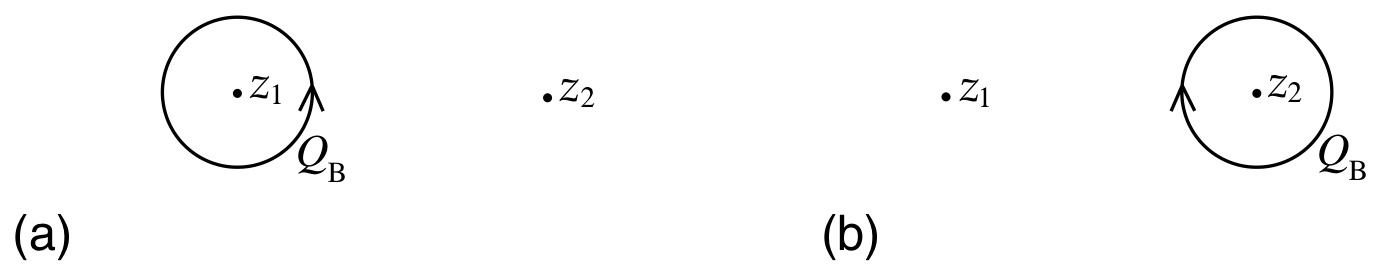
\includegraphics[width=0.8\textwidth]{figure/Fig12.2.jpg}
	\caption{Moving the PCO. The contour around $z_1$ in (a) is pulled around the sphere until it becomes a contour around $z_2$ in (b).}
	\label{fig:12.2}
\end{figure}

Consider now
\begin{equation}
	\lim_{z\to 0}\mathcal{X}(z)\,V_{-1}(0) \:, \label{12.5.11}
\end{equation}
where for convenience we concentrate on the holomorphic side. The $-1$ picture vertex operator is $\me^{-\phi}\mathcal{O}$ with $\mathcal{O}$ a matter superconformal primary. Consider now the term in $\mathcal{X}(z)$ that involves the matter fields,
\begin{equation}
	\me^{\phi}T_{\mathrm{F}}^{\mathrm{m}}(z)\,\me^{-\phi}\mathcal{O}(0) = z\,T_{\mathrm{F}}^{\mathrm{m}}(z)\,\mathcal{O}(0) + \mathcal{O}(z^2) \:. \label{12.5.12}
\end{equation}
The $z \to 0$ limit picks out the coefficient of the $z^{-1}$ in the matter OPE, which is precisely $G_{-1/2}\cdot \mathcal{O} = V_0$, the $0$ picture vertex operator. The purely ghost terms in $\mathcal{X}$ vanish as $z \to 0$, so that
\begin{equation}
	\lim_{z\to 0}\mathcal{X}(z)\,V_{-1}(0) = V_0(0) \:. \label{12.5.13}
\end{equation}

\begin{tcolorbox}[breakable]
	\begin{remark}
		\textbf{Derivation of \eqref{12.5.12} and \eqref{12.5.13}.} \textbf{Conventions.} In bosonized form the PCO is $\mathcal X=\me^{\phi}T_{F}^{\mathrm m}+c\,\partial\xi+\frac14\partial\eta\,\me^{2\phi}b+\frac14\partial(\eta\me^{2\phi}b)$. This is Polchinski's form, the translation of \eqref{12.5.4} through \eqref{12.5.5} and \eqref{12.5.7}. The fixed $-1$ picture vertex operator is $c\,\me^{-\phi}\mathcal O$, where $\mathcal O$ is a weight-$\frac12$ superconformal primary. Then
		\begin{align*}
			\me^{\phi}T_{F}^{\mathrm m}(z)\;c\,\me^{-\phi}\mathcal O(0)
			&\eqs{1} z\,c(0)\,T_{F}^{\mathrm m}(z)\mathcal O(0)\bigl(1+\dots\bigr)\\
			&\eqs{2} z\,c\Bigl[\frac{(G_{1/2}\cdot\mathcal O)}{z^{2}}+\frac{(G_{-1/2}\cdot\mathcal O)}{z}+\text{regular}\Bigr]
			\eqs{3} c\,V_{0}(0)+\dots ,\\
			c\,\partial\xi(z)\;c\,\me^{-\phi}\mathcal O(0)&\eqs{4} \text{vanishes as } z\to0 ,\\
			\bigl(\eta\,\me^{2\phi}b\bigr)(z)\;c\,\me^{-\phi}\mathcal O(0)&\eqs{5} \pm z\,\gamma\mathcal O(0)+\dots .
		\end{align*}
		At (1), $\me^{\phi}(z)\me^{-\phi}(0)\sim z^{-(1)(-1)}=z$. At (2), the OPE of $T_{F}^{\mathrm m}$ with the weight-$\frac12$ operator $\mathcal O$ has poles of order at most $2$, with coefficients $G_{r}\cdot\mathcal O$. At (3), $G_{1/2}\cdot\mathcal O=0$ for a primary, which leaves $G_{-1/2}\cdot\mathcal O=V_{0}$. At (4), $c(z)c(0)\sim z\,c\partial c(0)$ vanishes linearly, and $\partial\xi\,\me^{-\phi}$ is nonsingular. At (5), $\me^{2\phi}(z)\me^{-\phi}(0)\sim z^{2}\me^{\phi}(0)$ and $b(z)c(0)\sim1/z$, and $\eta\,\me^{\phi}=\gamma$. The term $\frac14\partial\eta\,\me^{2\phi}b$ therefore vanishes as $z\to0$. The total derivative $\frac14\partial(\eta\me^{2\phi}b)$, however, leaves a finite ghost term proportional to $\gamma\mathcal O$. Thus $\lim_{z\to0}\mathcal X(z)\,c\me^{-\phi}\mathcal O(0)=c\,V_{0}(0)+(\text{const})\,\gamma\mathcal O(0)$. The matter content is $V_{0}$, which is \eqref{12.5.13} in the old covariant form used in the text, where only the matter part is kept. The extra $\gamma\mathcal O$ term is the ghost completion that makes the $0$ picture fixed vertex operator BRST invariant. Its sign and normalization depend on the cocycle conventions and are not fixed here. So the statement in the text that the purely ghost terms vanish is true for the matter factor, not for the full BRST vertex operator.
	\end{remark}
\end{tcolorbox}

In the bosonic $n$-point amplitude with two $-1$ picture operators and $(n-2)$ $0$ picture operators, we can pull a PCO out of each of the latter to be left with $(n-2)$ PCOs and $n$ vertex operators, all of which are in the $-1$ picture. This is the `natural' picture, the one given by the state--operator mapping. This also shows how to define a general tree-level amplitude, with $n_{\mathrm{B}}$ bosons and $n_{\mathrm{F}}$ (which must be even) fermions. Put all the bosons in the natural $-1$ picture, all the fermions in the natural $-1/2$ picture, and include $(n_{\mathrm{B}} + \frac{1}{2}n_{\mathrm{F}} - 2)$ PCOs. By taking some of the PCOs coincident with vertex operators, possibly more than one PCO at the same vertex operator, one obtains a representation with the vertex operators in higher pictures.

Finally, let us tie up a loose end. The operator product \eqref{12.4.18} is just the product of two spacetime supersymmetry currents, $V_{\alpha} \equiv j_{\alpha}$. By the Ward identity and the supersymmetry algebra, we would expect the $z^{-1}$ term to be the translation current. Instead it is $\me^{-\phi}\psi^{\mu}$. However, this is the zero-momentum vector vertex operator in the $-1$ picture; if we move a PCO to the operator we get the $0$ picture $\del X^{\mu}$ which is indeed the translation current. So the algebra is correct. The $(1,0)$ operator $\me^{-\phi}\psi^{\mu}$ is the translation current; which picture it appears in has no effect on the physics.

\subsection*{Super-Riemann Surfaces}

The preceding discussion suggests a natural generalization to all orders of perturbation theory. That is, string amplitudes are given by an integral over moduli space and the ghost plus matter path integral with the following insertions: the appropriate vertex operator for each incoming or outgoing string in the natural $-1$ or $-1/2$ picture, the $b$-ghosts for the measure on moduli space as in the bosonic string, plus the appropriate number of PCOs to give a sensible path integral. At genus $g$, the Riemann--Roch theorem gives the number of $\beta$ zero modes minus the number of $\gamma$ zero modes as $2g - 2$. Equivalently, the total $\phi$ charge of the insertions must be $2g - 2$. To obtain this, the total number of PCOs must be
\begin{equation}
	n_{\mathcal{X}} = 2g - 2 + n_{\mathrm{B}} + \frac{n_{\mathrm{F}}}{2} \:, \label{12.5.14}
\end{equation}
at arbitrary points; this is for the open string or one side of the closed string. The same formal arguments as in the case of the bosonic string show that this defines a consistent unitary theory. In particular, the PCOs are BRST-invariant and do not affect the decoupling of null states.

\begin{tcolorbox}[breakable]
	\begin{remark}
		\textbf{Derivation of \eqref{12.5.14}.} The Riemann--Roch theorem for holomorphic weight-$\lambda$ fields on a genus-$g$ surface states that the number of zero modes of the weight-$\lambda$ field minus that of its weight-$(1-\lambda)$ partner is $(2\lambda-1)(g-1)$. For $\beta$ ($\lambda=\frac32$) and $\gamma$ ($1-\lambda=-\frac12$) this gives
		\begin{align*}
			n_{\beta}-n_{\gamma}&\eqs{1} (2\cdot\tfrac32-1)(g-1)=2g-2 ,\\
			\sum_{\text{insertions}}q_{\phi}&\eqs{2} 2g-2 ,\qquad\text{i.e.}\qquad n_{\mathcal X}-n_{\mathrm B}-\tfrac12n_{\mathrm F}=2g-2 ,\\
			n_{\mathcal X}&\eqs{3} 2g-2+n_{\mathrm B}+\tfrac12n_{\mathrm F} .
		\end{align*}
		At (1), the Riemann--Roch index was evaluated. At (2), each $\beta$ zero mode needs a $\delta(\beta)\cong\me^{+\phi}$ and each $\gamma$ zero mode a $\delta(\gamma)\cong\me^{-\phi}$ for a nonzero, finite path integral. In bosonized language, the anomaly in the $\phi$ current requires total $\phi$-charge $2g-2$, which is $-2$ on the sphere as used in section~12.4. The PCO carries $+1$ through $\delta(\beta)\cong\me^{\phi}$, a natural NS vertex operator carries $-1$, and a natural R vertex operator carries $-\frac12$. The extra $\xi$ insertion has $\phi$-charge $0$. At (3), the equation was solved for $n_{\mathcal X}$. For $g=0$ and $n_{\mathrm B}=n$ this gives $n-2$ PCOs, as in the tree-level discussion above.
	\end{remark}
\end{tcolorbox}

This prescription is sufficient for all the calculations we will carry out. However, in the remainder of this section we will develop superstring perturbation theory from a more general and geometric point of view. One reason for this is that the picture-changing prescription is rather ad hoc and it would be satisfying to see it derived in some way. Another is that this prescription actually has a subtle ambiguity at higher genus, which is best resolved from the more geometric point of view.

The needed idea is supermoduli space, the space of super-Riemann surfaces (SRSs). These are defined by analogy to Riemann surfaces. Cover the surface with overlapping coordinate patches. The $m$th has coordinates $z_m, \theta_m$. Patches are glued together with superconformal transformations. That is, if patches $m$ and $n$ overlap, identify points such that
\begin{subequations} \label{12.5.15}
	\begin{align}
		z_m &= f_{mn}(z_n) + \theta_n\,g_{mn}(z_n)\,h_{mn}(z_n) \:, \label{12.5.15a} \\
		\theta_m &= g_{mn}(z_n) + \theta_n\,h_{mn}(z_n) \:, \label{12.5.15b} \\
		h_{mn}^2(z_n) &= \del_z f_{mn}(z_n) + g_{mn}(z_n)\,\del_z g_{mn}(z_n) \:. \label{12.5.15c}
	\end{align}
\end{subequations}
\begin{tcolorbox}[breakable]
	\begin{remark}
		\textbf{Derivation of \eqref{12.5.15c}.} A superconformal transition function satisfies \eqref{12.3.6}, $D_{\theta}z_{m}=\theta_{m}D_{\theta}\theta_{m}$, with $D_{\theta}=\partial_{\theta}+\theta\partial_{z}$ acting on the $(z_{n},\theta_{n})$ coordinates, written $(z,\theta)$ here. Suppress the indices $mn$. For $z_{m}=f+\theta gh$ and $\theta_{m}=g+\theta h$,
		\begin{align*}
			D_{\theta}z_{m}&\eqs{1} gh+\theta\,\partial f ,\qquad
			D_{\theta}\theta_{m}\eqs{1} h+\theta\,\partial g ,\\
			\theta_{m}D_{\theta}\theta_{m}&=(g+\theta h)(h+\theta\partial g)
			\eqs{2} gh+\theta\bigl(h^{2}-g\,\partial g\bigr) .
		\end{align*}
		At (1), $\partial_{\theta}(\theta gh)=gh$ and $\theta\partial_{z}(\theta gh)=0$ because $\theta^{2}=0$. At (2), $g\theta\partial g=-\theta g\partial g$, since the odd quantities $g$ and $\theta$ anticommute, and $\theta h\theta\partial g=0$. The $\theta^{0}$ terms agree automatically. Equating the $\theta^{1}$ terms gives $\partial f=h^{2}-g\partial g$, that is
		\[
		\boxed{\;h^{2}=\partial_{z}f+g\,\partial_{z}g\;}
		\]
		which is \eqref{12.5.15c}. This is the patch-to-patch version of \eqref{12.3.9b}. The same computation checks the sphere gluing \eqref{12.5.18}: for $u=1/z$ and $\phi=\mi\theta/z$, $D_{\theta}u=\theta\partial_{z}(1/z)=-\theta/z^{2}$ and $\phi D_{\theta}\phi=(\mi\theta/z)(\mi/z)=-\theta/z^{2}$, so the two agree. It also checks the torus identification \eqref{12.5.21} and the SCKV \eqref{12.5.22}: for $z'=z+\theta\epsilon$ and $\theta'=\theta+\epsilon$, $D_{\theta}z'=\epsilon+\theta$ and $\theta'D_{\theta}\theta'=(\theta+\epsilon)\cdot1$, which are equal. This is the case $f=z$, $g=\epsilon$, $h=1$ of \eqref{12.5.15}.
	\end{remark}
\end{tcolorbox}
\noindent The holomorphic functions $f_{mn}$ and the anticommuting holomorphic functions $g_{mn}$ define the SRS. Two SRSs are equivalent if there is a one-to-one mapping between them such that the respective coordinates are related by a superconformal transformation. Tensor fields are defined by analogy to tensors on an ordinary manifold, as functions in each patch with appropriate transformations between patches. Supermoduli space is the set of equivalence classes of super-Riemann surfaces. The coordinates on supermoduli space are the bosonic (even) moduli $t_j$ and the anticommuting (odd) moduli $\nu_a$. The Riemann--Roch theorem gives the number of odd moduli minus the number of globally defined odd superconformal transformations as $2g - 2$.

Again one can define all of this by Taylor expanding all functions in the anticommuting variables $\theta$ and $\nu_a$. The term in $f_{mn}$ of order $\nu_a^0$ defines an ordinary (not super-) Riemann surface, and everything is expressed in terms of functions on this surface with the component form of the superconformal transformation between patches. Incidentally, $z$ and $\bar{z}$ are no longer formally conjugates of one another on a SRS, particularly in the heterotic string where $\bar{z}$ transforms as the conjugate of equation \eqref{12.5.15} while $z$ transforms as on a `bosonic' Riemann surface. However, if one defines everything by the Taylor expansion then $z$ and $\bar{z}$ are again conjugates on the resulting ordinary Riemann surface.

For any SRS, setting the $\nu_a$ to zero makes the anticommuting $g_{mn}$ vanish and leaves
\begin{subequations} \label{12.5.16}
	\begin{align}
		z_m &= f_{mn}(z_n) \:, \label{12.5.16a} \\
		\theta_m &= \theta_n\,h_{mn}(z_n) \:, \quad h_{mn}^2(z_n) = \del_z f_{mn}(z_n) \:. \label{12.5.16b}
	\end{align}
\end{subequations}
The transformation of $z$ defines a Riemann surface, but that of $\theta$ requires the additional choice of which square root to take in each $h_{mn}$. This choice is known as a spin structure; it is the same data one would need to put a spin-$1/2$ field on the surface. The signs are not all independent. If three patches overlap then the transition functions must satisfy the cocycle condition
\begin{equation}
	h_{mn}\,h_{np}\,h_{pm} = 1 \:. \label{12.5.17}
\end{equation}
Also, a coordinate change $\theta_p \to -\theta_p$ in the patch $p$ changes the signs of all the $h_{pn}$. The net result is that there is one meaningful sign for each nontrivial closed path on the surface, $2g$ for a genus $g$ surface. These define $2^{2g}$ different spin structures, topologically distinct ways to put a spinor field on the surface.

Any sphere is equivalent to the one with two patches $(z,\theta)$, $(u,\phi)$ and transition functions
\begin{equation}
	u = \frac{1}{z} \:, \quad \phi = \frac{\mi\theta}{z} \:. \label{12.5.18}
\end{equation}
Clearly there is just one spin structure. The index theorem implies superconformal Killing transformations. One can look for infinitesimal transformations as in the bosonic case, with the result that $\delta f$ must be at most quadratic in $z$ and $\delta g$ linear in $z$. The general finite transformation is then of the superconformal form with
\begin{equation}
	f(z) = \frac{\alpha z + \beta}{\gamma z + \delta} \:, \quad g(z) = \frac{\epsilon_1 + \epsilon_2 z}{\gamma z + \delta} \:, \label{12.5.19}
\end{equation}
with $\alpha\delta - \beta\gamma = 1$. In particular there are two odd transformations, $\epsilon_1$ and $\epsilon_2$, consistent with the Riemann--Roch theorem. These can be used to fix the odd coordinates of two NS vertex operators to zero.

\begin{tcolorbox}[breakable]
	\begin{remark}
		\textbf{Derivation of the sphere SCKVs \eqref{12.5.19}.} \textbf{Conventions.} An infinitesimal superconformal transformation is generated by an even vector field $v(z)$, a tensor of weight $-1$, and an odd field $\eta(z)$ of weight $-\frac12$, as in \eqref{12.3.10}: $\delta z=\epsilon[v-\mi\theta\eta]$ and $\delta\theta=\epsilon[-\mi\eta+\frac12\theta\partial v]$. Such a transformation is a globally defined SCKV if it is regular in both patches of \eqref{12.5.18}. Transforming to the $(u,\phi)$ patch,
		\begin{align*}
			\delta u&=-\frac{\delta z}{z^{2}}\eqs{1} -\epsilon\,u^{2}\,v(1/u)+\cdots ,\\
			\delta\phi&=\frac{\mi\,\delta\theta}{z}-\frac{\mi\theta\,\delta z}{z^{2}}\eqs{2} \epsilon\,u\,\eta(1/u)+\theta\text{-dependent terms} .
		\end{align*}
		At (1), $u=1/z$. At (2), the odd part of $\delta z$ is proportional to $\theta$, so the second term is regular. Regularity at $u=0$ therefore requires $u^{2}v(1/u)$ and $u\,\eta(1/u)$ to be regular. So $v$ is at most quadratic and $\eta$ at most linear:
		\[
		v=a_{0}+a_{1}z+a_{2}z^{2},\qquad \eta=\epsilon_{1}+\epsilon_{2}z .
		\]
		That is three even and two odd parameters. Exponentiating gives the Möbius $f$ of \eqref{12.5.19} together with $g=(\epsilon_{1}+\epsilon_{2}z)/(\gamma z+\delta)$. The denominator is needed because $g$ has weight $-\frac12$: under the even Möbius part it transforms with $(\partial f)^{1/2}=(\gamma z+\delta)^{-1}$. Riemann--Roch, in the form of the box after \eqref{12.5.14}, predicts $(\#\text{odd moduli})-(\#\text{odd SCKVs})=2g-2=-2$ at $g=0$. There are no odd moduli, so there are $2$ odd SCKVs, in agreement.
	\end{remark}
\end{tcolorbox}

A torus can be described as the $(z,\theta)$ plane modded by a group of rigid superconformal transformations,
\begin{equation}
	(z,\theta) \cong (z + 2\pi, \eta_1\theta) \cong (z + 2\pi\tau, \eta_2\theta) \:. \label{12.5.20}
\end{equation}
The $\eta_1$ and $\eta_2$ are each $\pm 1$, defining the four spin structures. When $\theta$ changes sign around a loop, the bosonic and fermionic components of any superfield will have opposite periodicities, and in particular $T_{\mathrm{F}}$ will be antiperiodic. We thus denote the spin structures $(\mathrm{P},\mathrm{P})$, $(\mathrm{P},\mathrm{A})$, $(\mathrm{A},\mathrm{P})$, and $(\mathrm{A},\mathrm{A})$, giving the $z \to z + 2\pi$ periodicity first. The periodicities on the right-moving side have the same form, with $\bar{\tau}$ the conjugate of $\tau$ but with independent $\tilde{\eta}_1$ and $\tilde{\eta}_2$.

On a torus the only holomorphic functions are the constants, so $\beta$ and $\gamma$ zero modes are possible only in the $(\mathrm{P},\mathrm{P})$ case, in which case there is one of each. There is then an odd supermodulus $\nu$, giving rise to the more general periodicity
\begin{equation}
	(z,\theta) \cong (z + 2\pi, \theta) \cong (z + 2\pi\tau + \theta\nu, \theta + \nu) \:. \label{12.5.21}
\end{equation}
There is also the superconformal Killing vector (SCKV)
\begin{equation}
	(z,\theta) \longrightarrow (z + \theta\epsilon, \theta + \epsilon) \:. \label{12.5.22}
\end{equation}
The number of odd moduli minus the number of SCKVs is zero in all sectors, being $1 - 1$ for the $(\mathrm{P},\mathrm{P})$ spin structure and $0 - 0$ for the others. The modular group and the fundamental region for $\tau$ are the same as in the bosonic string.

Returning to a general SRS, if the positions of $n$ vertex operators are singled out then there is a nontrivial closed curve circling each, less one, giving $2^{2g+n-1}$ spin structures altogether. The additional spin structures come from the choice of R or NS boundary conditions of the external strings. To describe the supermoduli space of SRSs with $n_{\mathrm{B}}$ NS vertex operators and $n_{\mathrm{F}}$ R vertex operators, it is useful to extend the approach used in section 5.4. First in the bosonic case, consider a specific patching together of a Riemann surface, with $n$ marked points. We will define another Riemann surface as equivalent to this one if there is a one-to-one holomorphic mapping between the two which leaves the coordinates of the points invariant. That is, $f(z) - z$ must vanish linearly at the vertex operators. For simplicity we take each operator to be at $z = 0$ in its own tiny patch. Since we are modding by a smaller group, with two real conditions for each vertex operator, we obtain a correspondingly larger coset space, with two additional moduli for each vertex operator. This is similar to the treatment of vertex operator positions in section 5.4, but more abstract. In the superconformal case, we mod out the superconformal transformations for which $f(z) - z$ and $g(z)$ vanish linearly at each NS vertex operator. At each R vertex operator, $g(z)$ has a branch cut, and so it is appropriate to require $f(z) - z$ to vanish linearly in $z$ and $g(z)$ to vanish as $z^{1/2}$. The NS vertex reduces the odd coordinate degrees of freedom by one and so increases the number of inequivalent surfaces: the number of odd moduli increases by one, which we can take to be the $\theta$ coordinate of the operator. The condition for the R vertex operator is essentially half as restrictive, so that there is an additional odd modulus for each pair of R vertex operators. This has no simple interpretation as a vertex operator position; an R vertex operator produces a branch cut in $\theta$, so there can be no well-defined $\theta$ coordinate for the operator. The total number of odd moduli is
\begin{equation}
	n_{\nu} = 2g - 2 + n_{\mathrm{B}} + \frac{n_{\mathrm{F}}}{2} \:. \label{12.5.23}
\end{equation}

\begin{tcolorbox}[breakable]
	\begin{remark}
		\textbf{Derivation of \eqref{12.5.23}.} Odd moduli are odd deformations of the gluing, $\beta$-type zero modes of weight $\frac32$. Odd SCKVs are globally defined $\eta$'s of weight $-\frac12$, $\gamma$-type zero modes. Without punctures, Riemann--Roch, as in the box after \eqref{12.5.14}, gives
		\begin{align*}
			n_{\nu}-n_{\eta}&\eqs{1} 2g-2 ,\\
			n_{\nu}-n_{\eta}&\eqs{2} 2g-2+n_{\mathrm B}\cdot1+n_{\mathrm F}\cdot\tfrac12 ,\\
			n_{\nu}&\eqs{3} 2g-2+n_{\mathrm B}+\tfrac12n_{\mathrm F} .
		\end{align*}
		At (1), Riemann--Roch was applied with $\lambda=\frac32$. At (2), each NS puncture imposes $g(z)=\mathcal O(z)$ on the allowed transformations, one odd condition, so the number of inequivalent odd deformations grows by one. Each R puncture imposes only $g(z)=\mathcal O(z^{1/2})$. Its contribution is half as large, and R punctures come in pairs, since the $\theta$ branch cuts must pair up for the spin structure to be defined. At (3), for amplitudes the punctures remove all odd SCKVs, so $n_{\eta}=0$. For example, the sphere has $n_{\eta}=2$ without punctures, and two NS punctures already fix both. The result \eqref{12.5.23} coincides with the PCO count \eqref{12.5.14}.
	\end{remark}
\end{tcolorbox}

\subsection*{The Measure on Supermoduli Space}

The expression \eqref{5.4.19} for the bosonic string S-matrix now generalizes in a natural way,
\begin{equation}
	\mathcal{S}(1;\dots;n) = \sum_{\chi,\gamma}\me^{-\lambda\chi}\frac{1}{n_{\mathrm{R}}}\int_{\mathfrak{M}_{\chi,\gamma}}\dif^{n_{\mathrm{e}}}t\,\dif^{n_{\mathrm{o}}}\nu\:\biggl\langle \prod_{j=1}^{n_{\mathrm{e}}}B_{j}\prod_{a=1}^{n_{\mathrm{o}}}\delta(B_{a})\prod_{i=1}^{n}\hat{\mathcal{V}}_{i}\biggr\rangle \:. \label{12.5.24}
\end{equation}
The sum is over topologies $\chi$ and spin structures $\gamma$. The integral runs over the corresponding supermoduli space. There are $n_{\mathrm{e}}$ even moduli, $n_{\mathrm{o}}$ odd moduli, and $n$ external strings. The quantity $B_j$ in the ghost insertions is
\begin{equation}
	B_{j} = \sum_{(mn)}\oint_{C_{mn}}\frac{\dif z_m\dif\theta_m}{2\pi\mi}\,B(z_m,\theta_m)\biggl(\frac{\del z_m}{\del t_j} - \frac{\del\theta_m}{\del t_j}\,\theta_m\biggr)_{z_n,\theta_n} \:, \label{12.5.25}
\end{equation}
plus a right-moving piece of the same form; $B_a$ is given by an identical expression with $\nu_a$ replacing $t_j$. The sum again runs over all pairs of overlapping patches $m$ and $n$, clockwise as seen from $m$, with the $z_m$ integration along a contour between the two patches and the $\theta_m$ integral of the usual Berezin form. The $B$ ghost superfield is as in equation \eqref{12.3.25}, $B = \beta + \theta b$.

The logic of this expression is the same as for the earlier bosonic expression. First, the number of commuting and anticommuting ghost insertions is correct for a well-defined path integral. Second, the path integral depends only on the superconformal structure and not on the particular choice of patches and transition functions. In particular it is unchanged if we make a superconformal transformation within a single coordinate patch. The combination $\del z_m + (\del\theta_m)\theta_m$ transforms as a $(-1,0)$ tensor superfield, so the integrand is a $(1/2,0)$ tensor superfield and the integral is invariant. Third, under a change of coordinates in supermoduli space, the product $\prod_{j=1}^{n_{\mathrm{e}}}B_j \prod_{a=1}^{n_{\mathrm{o}}}\delta(B_a)$ transforms as a density, inversely to the measure on supermoduli space. Finally, the commutator of the BRST charge with $B_{j,a}$ is $T_{j,a}$, defined in the same way but with $B$ replaced by
\begin{equation}
	Q_{\mathrm{B}}\cdot B(z) = T(z) = T_{\mathrm{F}}(z) + \theta\,T_{\mathrm{B}}(z) \:. \label{12.5.26}
\end{equation}
The insertion of $T_{j,a}$ generates a relative coordinate transformation of adjacent patches, which is just the derivative with respect to the supermodulus of the worldsheet.

It is interesting to work out the form of the amplitude more explicitly for a special choice of patches and transition functions. Namely, let patch 1 be contained entirely within patch 2, so that the overlap is an annulus. Let the 1-2 transition functions depend only on a single odd modulus $\nu$, as follows:
\begin{equation}
	f_{12}(z_2) = z_2 \:, \quad g_{12}(z_2) = \nu\,\alpha(z_2) \:, \label{12.5.27}
\end{equation}
for some holomorphic function $\alpha(z)$. The ghost factor \eqref{12.5.25} is proportional to
\begin{equation}
	B[\alpha] = \oint \frac{\dif z_1}{2\pi\mi}\,\alpha(z_1)\,\beta(z_1) \:. \label{12.5.28}
\end{equation}
Similarly the path integral depends on $\nu$ only through the insertion
\begin{equation}
	\nu\,T[\alpha] \:, \label{12.5.29}
\end{equation}
where $\beta$ is replaced by $T_{\mathrm{F}}$. We can then perform the integration over $\nu$, so that the net effect of the supermodulus is the insertion in the path integral of
\begin{equation}
	T[\alpha]\,\delta(B[\alpha]) = Q_{\mathrm{B}}\cdot \Theta(B[\alpha]) \:. \label{12.5.30}
\end{equation}
The function $\alpha(z_1)$ is holomorphic in the annular overlap of the patches, but in general cannot be extended holomorphically into the full inner patch $z_1$. If it can, the contour integrals $B[\alpha]$ and $T[\alpha]$ vanish. In this case $\nu$ is not a modulus at all because it can be transformed away. A nontrivial case is
\begin{equation}
	\alpha(z_1) = \frac{1}{z_1 - z_0} \:, \label{12.5.31}
\end{equation}
for which $B[\alpha] = \beta(z_0)$ and the insertion \eqref{12.5.30} just becomes the PCO $\mathcal{X}(z_0)$ (the second term in $\mathcal{X}$ is from normal ordering). Thus, the PCO is the result of integrating out an odd modulus in this special parameterization of the SRSs. Note that the number \eqref{12.5.23} of odd moduli is the same as the number \eqref{12.5.14} of PCOs needed in the ad hoc approach. This provides the desired geometric derivation of the picture-changing prescription.

\begin{tcolorbox}[breakable]
	\begin{remark}
		\textbf{Derivation of \eqref{12.5.30} and of the PCO from \eqref{12.5.31}.} \textbf{Conventions.} $\nu$ is a single odd modulus with Berezin integral $\int\dif\nu\,\nu=1$, and $B[\alpha]$ is Grassmann even, since $\beta$ is commuting. The $\nu$-dependence of the path integral enters only through the insertion $\exp(\nu T[\alpha])=1+\nu T[\alpha]$. Then
		\begin{align*}
			\int\dif\nu\,\bigl(1+\nu T[\alpha]\bigr)\,\delta\bigl(B[\alpha]\bigr)
			&\eqs{1} T[\alpha]\,\delta\bigl(B[\alpha]\bigr)
			\eqs{2} \bigl(Q_{\mathrm B}\cdot B[\alpha]\bigr)\,\Theta'\bigl(B[\alpha]\bigr)\\
			&\eqs{3} Q_{\mathrm B}\cdot\Theta\bigl(B[\alpha]\bigr) ,\\
			B[\alpha]=\oint_{z_{0}}\frac{\dif z_{1}}{2\pi\mi}\,\frac{\beta(z_{1})}{z_{1}-z_{0}}
			&\eqs{4} \beta(z_{0}) ,\qquad T[\alpha]\eqs{4} T_{F}(z_{0}) ,\\
			T[\alpha]\,\delta\bigl(B[\alpha]\bigr)&=T_{F}(z_{0})\,\delta\bigl(\beta(z_{0})\bigr) .
		\end{align*}
		At (1), the Berezin integral picks out the term linear in $\nu$. At (2), \eqref{12.5.26} gives $Q_{\mathrm B}\cdot\beta=T_{F}$, hence $Q_{\mathrm B}\cdot B[\alpha]=T[\alpha]$, and $\delta=\Theta'$. At (3), the chain rule was used: $Q_{\mathrm B}$ acts as a derivation on functions of the commuting operator $B[\alpha]$. At (4), $\alpha=1/(z_{1}-z_{0})$ is holomorphic in the annulus but has a pole at $z_{0}$ inside patch $1$. Shrinking the contour onto $z_{0}$ picks the residue. If instead $\alpha$ extended holomorphically into patch $1$, the integrand would be holomorphic inside and $B[\alpha]=T[\alpha]=0$. The final product $T_{F}\delta(\beta)$ is the first term of $\mathcal X$ in \eqref{12.5.4}. The second term, $-\partial b\,\delta'(\beta)$, is the normal-ordering correction that arises when $T_{F}(z_{0})$ and $\delta(\beta(z_{0}))$ are brought to the same point, as in the box after \eqref{12.5.8}.
	\end{remark}
\end{tcolorbox}

The parameterization \eqref{12.5.27} is always possible locally on supermoduli space. It can also be used globally, with careful treatment of the modular identification and the limits of moduli space. There is a literature on the `ambiguity of superstring perturbation theory,' which arose from parameterizations that did not precisely cover supermoduli space. It appears that superstring perturbation theory to arbitrary order is understood in principle, and certain special amplitudes have been calculated at higher orders of perturbation theory. However, the subject is somewhat unfinished --- a fully explicit proof of the perturbative consistency of the theory seems to be lacking. With the immense progress in nonperturbative string theory, filling this technical gap does not seem to be a key issue.

We derived the bosonic version \eqref{5.4.19} of the measure \eqref{12.5.24} by starting with a path integral over the worldsheet metric, whereas in the present case we have written it down directly. One can partly work backwards to an analogous description as follows. Although $\alpha(z_1)$ cannot be extended holomorphically into patch 1 it can be extended smoothly. It can then be removed by a change of variables in the path integral, but not one that leaves the action invariant. The odd modulus $\nu$ appears in the final action, multiplying $T_{\mathrm{F}}$ and a function that can be regarded as the worldsheet gravitino field. In particular, the PCO can be regarded as coming from a pointlike gravitino, a gauge where the gravitino has delta-function support.

\section{One-Loop Amplitudes}

We will illustrate one-loop superstring calculations with two examples where the low energy limit can be obtained in closed form.

The first is the heterotic string amplitude with four gauge bosons and one antisymmetric tensor. The Green--Schwarz anomaly cancellation requires a one-loop Chern--Simons term
\begin{equation}
	\int B_{\textit{2}}\wedge \operatorname{Tr}_{\mathrm{v}}(F_{\textit{2}}^4) \:. \label{12.6.1}
\end{equation}
We would like to confirm the appearance of this term by an explicit string calculation.

Note first that this can only arise from the $(\mathrm{P},\mathrm{P})$ path integral. This is because it is odd under spacetime parity: written out in components, it involves the ten-dimensional $\epsilon$-tensor. The heterotic string worldsheet action and constraints are invariant under parity. The parity asymmetry of the theory, the fact that the massless fermions are in a $\mathbf{16}$ and not a $\mathbf{16}'$, comes about from the GSO projection in the right-moving R sector, the choice of $\exp(\pi\mi\tilde{F})$ to be $+1$ or $-1$. The $(\mathrm{P},\mathrm{P})$ path integral produces this term in the projection operator. The path integral is then
\begin{align}
	&\quad \Bigl(\frac{2}{\alpha'}\Bigr)^{5/2}g_{\mathrm{c}}^5 \int_{\mathcal{F}}\frac{\dif\tau\dif\bar{\tau}}{8\tau_2}\prod_{i=1}^{5}\int\dif^2 w_i \:\biggl\langle b(0)\tilde{b}(0)\tilde{c}(0)c(0)\,\mathcal{X}(0) \nonumber \\
	&\quad \times \prod_{i=1}^{4}\hat{k}^{-1/2}j^{a_i}\Bigl(\mi e_i\cdot\bar{\del}X + \frac{1}{2}\alpha' k_i\cdot\tilde{\psi}\,e_i\cdot\tilde{\psi}\Bigr)\me^{\mi k_i\cdot X(w_i,\bar{w}_i)} \nonumber \\
	&\quad \times \mi e_{5\mu\nu}\del X^\mu\,\delta(\tilde{\gamma})\,\tilde{\psi}^\nu\,\me^{\mi k_5\cdot X(w_5,\bar{w}_5)}\biggr\rangle_{(\mathrm{P},\mathrm{P})} \:. \label{12.6.2}
\end{align}
The $bc$ ghosts and corresponding measure are the same as in the bosonic string, with an extra $1/2$ from the GSO projection operator. For the $(\mathrm{P},\mathrm{P})$ spin structure there is one PCO and one $-1$ picture vertex operator.

We will consider in order the $\tilde{\psi}^\mu$, $X^\mu$, $bc$, $\beta\gamma$, and $j^a$ path integrals. In the vacuum amplitude the $\tilde{\psi}^\mu$ path integral vanishes in the $(\mathrm{P},\mathrm{P})$ sector. In terms of a trace, this is due to a cancellation between the R sector ground states. In terms of a path integral it is due to the Berezin integration over the zero mode of $\psi^\mu$ (which exists only for this spin structure). In the latter form it is clear that we need at least ten factors of $\tilde{\psi}$ to obtain a nonzero path integral. In fact, the path integral \eqref{12.6.2} has a maximum of ten $\tilde{\psi}$s, including one from the term
\begin{equation}
	\delta(\tilde{\beta})\,\mi\Bigl(\frac{2}{\alpha'}\Bigr)^{1/2}\tilde{\psi}^\rho\bar{\del}X_\rho \label{12.6.3}
\end{equation}
in the PCO. The relevant path integral is easily obtained from a trace, giving
\begin{equation}
	\biggl\langle \prod_{i=1}^{10}\tilde{\psi}^{\mu_i}\biggr\rangle_{\tilde{\psi},(\mathrm{P},\mathrm{P})} = \epsilon^{\mu_1\dots\mu_{10}}\,\bar{q}^{10/24}\prod_{n=1}^{\infty}(1-\bar{q}^n)^{10} = \epsilon^{\mu_1\dots\mu_{10}}\bigl[\eta(\tau)^{10}\bigr]^* \:. \label{12.6.4}
\end{equation}

\begin{tcolorbox}[breakable]
	\begin{remark}
		\textbf{Derivation of \eqref{12.6.4}.} \textbf{Conventions.} The $(\mathrm P,\mathrm P)$ spin structure is the R sector, periodic in $\sigma^{1}$, with $\exp(\pi\mi\tilde F)$ inserted in the trace, periodic in $\sigma^{2}$. The ten zero modes $\tilde\psi_{0}^{\mu}$ satisfy $\{\tilde\psi_{0}^{\mu},\tilde\psi_{0}^{\nu}\}=\eta^{\mu\nu}$, so $\tilde\psi_{0}^{\mu}=\Gamma^{\mu}/\sqrt2$ on the ground states. The overall normalization of the zero-mode trace is fixed so that the coefficient of $\epsilon^{\mu_{1}\dots\mu_{10}}$ is $1$, as in Polchinski. Then
		\begin{align*}
			\Bigl\langle\prod_{i=1}^{10}\tilde\psi^{\mu_{i}}\Bigr\rangle_{(\mathrm P,\mathrm P)}
			&=\operatorname{Tr}_{\mathrm R}\Bigl[\me^{\pi\mi\tilde F}\,\bar q^{\tilde L_{0}-\tilde c/24}\,\tilde\psi_{0}^{\mu_{1}}\cdots\tilde\psi_{0}^{\mu_{10}}\Bigr]\\
			&\eqs{1} \bar q^{10(1/16-1/48)}\prod_{n=1}^{\infty}(1-\bar q^{n})^{10}\times\operatorname{tr}_{32}\bigl[\Gamma\,2^{-5}\Gamma^{\mu_{1}}\cdots\Gamma^{\mu_{10}}\bigr]\\
			&\eqs{2} \bar q^{10/24}\prod_{n=1}^{\infty}(1-\bar q^{n})^{10}\;\epsilon^{\mu_{1}\dots\mu_{10}}\\
			&=\bigl[\eta(\tau)^{10}\bigr]^{*}\epsilon^{\mu_{1}\dots\mu_{10}} .
		\end{align*}
		At (1), the trace factorizes into oscillators and zero modes. Each fermion contributes the R ground-state energy $\frac1{16}$ minus $\frac{c}{24}=\frac1{48}$. Each oscillator $\tilde\psi^{\mu}_{-n}$ contributes $1-\bar q^{n}$, where the minus sign comes from $\exp(\pi\mi\tilde F)$. On the zero modes $\exp(\pi\mi\tilde F)$ acts as the chirality matrix $\Gamma$. At (2), $\frac1{16}-\frac1{48}=\frac1{24}$. In $\operatorname{tr}(\Gamma\Gamma^{\mu_{1}}\cdots\Gamma^{\mu_{k}})$, fewer than ten distinct matrices give a product that is traceless. For $\mu_{i}$ a permutation of $0,\dots,9$, the trace is $\operatorname{sgn}\times\operatorname{tr}(\Gamma^{2})=\pm32$, which gives $\epsilon^{\mu_{1}\dots\mu_{10}}$ with the stated normalization. This is why at least ten $\tilde\psi$ insertions are needed, and why the result is parity odd.
	\end{remark}
\end{tcolorbox}

\noindent The $X^\mu$ path integral is then reduced to
\begin{equation}
	\biggl\langle \del X^\mu(w_5)\,\bar{\del}X^\rho(0)\prod_{i=1}^{5}\me^{\mi k_i\cdot X(w_i,\bar{w}_i)}\biggr\rangle_X \:, \label{12.6.5}
\end{equation}
the gradients coming from the tensor vertex operator and the PCO.

To make things simple we now take the $k_i \to 0$ limit. Contractions between the gradients and exponentials, and among the exponentials, are then suppressed. Only the contraction between the gradients survives, $-\alpha'/8\pi\tau_2$ from the background charge term $\alpha'(\operatorname{Im} w_{ij})^2/4\pi\tau_2$ in the Green's function \eqref{7.2.3}. The leading term in the expectation value \eqref{12.6.5} is then
\begin{align}
	&\quad -\mi(2\pi)^{10}\delta^{10}\Bigl(\sum_{i=1}^{5}k_i\Bigr)\frac{\eta^{\mu\rho}\alpha'}{8\pi\tau_2}(4\pi^2\alpha'\tau_2)^{-5}|\eta(\tau)|^{-20}(4\pi^2\alpha'\tau_2)^{10} \nonumber \\
	&= -\mi(2\pi)^{10}\delta^{10}\Bigl(\sum_{i=1}^{5}k_i\Bigr)\frac{\eta^{\mu\rho}\alpha'}{8\pi\tau_2}(4\pi^2\alpha'\tau_2)^5 |\eta(\tau)|^{20} \:. \label{12.6.6}
\end{align}

\begin{tcolorbox}[breakable]
	\begin{remark}
		\textbf{Derivation of \eqref{12.6.6}.} \textbf{Conventions.} $\langle X^{\mu}(w_{1})X^{\nu}(w_{2})\rangle=\eta^{\mu\nu}G'(w_{1},w_{2})$ with $G'$ the torus Green's function \eqref{7.2.3}. The noncompact $X$ path integral with momentum insertions is $\mi(2\pi)^{10}\delta^{10}(\sum k)\,Z_{X}$, where $Z_{X}=(4\pi^{2}\alpha'\tau_{2})^{-5}|\eta(\tau)|^{-20}$ is the torus partition function of ten bosons from chapter~7. At $k\to0$ only the contraction of the two gradients survives. Writing $w_{12}=w_{1}-w_{2}$,
		\begin{align*}
			\partial_{w_{1}}\partial_{\bar w_{2}}G'
			&\eqs{1} \partial_{w_{1}}\partial_{\bar w_{2}}\Bigl[\alpha'\frac{(\operatorname{Im}w_{12})^{2}}{4\pi\tau_{2}}\Bigr]
			=\frac{\alpha'}{4\pi\tau_{2}}\,\partial_{w_{1}}\partial_{\bar w_{2}}\Bigl[-\frac{(w_{12}-\bar w_{12})^{2}}{4}\Bigr]\\
			&\eqs{2} \frac{\alpha'}{4\pi\tau_{2}}\,\partial_{\bar w_{2}}\Bigl[-\frac{w_{12}-\bar w_{12}}{2}\Bigr]
			\eqs{3} -\frac{\alpha'}{8\pi\tau_{2}} .
		\end{align*}
		At (1), the $\vartheta_{1}$ term is the sum of a holomorphic and an antiholomorphic function of $w_{12}$, so the mixed derivative kills it away from $w_{1}=w_{2}$. At $w_{5}=0$ it leaves a contact term $\propto\delta^{2}(w_{5})$, where the PCO meets the tensor vertex operator. Following Polchinski this term is dropped, which amounts to keeping the PCO away from the vertex operators. The constant $k(\tau,\bar\tau)$ drops out. At (2), $\operatorname{Im}w_{12}=(w_{12}-\bar w_{12})/2\mi$ was used. At (3), $\partial_{\bar w_{2}}\bar w_{12}=-1$. So $\langle\partial X^{\mu}\bar\partial X^{\rho}\rangle=-\eta^{\mu\rho}\alpha'/8\pi\tau_{2}$, and
		\[
		\boxed{\;\langle\cdots\rangle_{X}=-\mi(2\pi)^{10}\delta^{10}\bigl(\textstyle\sum_i k_{i}\bigr)\frac{\eta^{\mu\rho}\alpha'}{8\pi\tau_{2}}\,(4\pi^{2}\alpha'\tau_{2})^{-5}\,|\eta(\tau)|^{-20}\;}
		\]
		This is the first line of \eqref{12.6.6} without the extra factor $(4\pi^{2}\alpha'\tau_{2})^{10}$. That factor, and with it the second line $(4\pi^{2}\alpha'\tau_{2})^{5}|\eta|^{20}$, appear to be misprints. The first line does not even equal the second, because the powers of $|\eta|$ differ. The box after \eqref{12.6.17} shows that only the boxed form gives the measure $\dif^{2}\tau/\tau_{2}^{2}$ and the function $\hat f=\eta^{-8}f$ of \eqref{12.6.16} and \eqref{12.6.17}.
	\end{remark}
\end{tcolorbox}

\noindent The $bc$ path integral is
\begin{equation}
	\langle b(0)\tilde{b}(0)\tilde{c}(0)c(0)\rangle_{bc} = |\eta(\tau)|^4 \:, \label{12.6.7}
\end{equation}
just as in the bosonic string. The $\beta\gamma$ path integral is the reciprocal of the right-moving part of this,
\begin{equation}
	\langle \delta(\tilde{\beta}(0))\delta(\tilde{\gamma}(\bar{w}_5))\rangle_{\beta\gamma} = \bigl[\eta(\tau)^{-2}\bigr]^* \:. \label{12.6.8}
\end{equation}

Finally for the current algebra, we need
\begin{equation}
	\hat{k}^{-2}\langle j^{a_1}(w_1)j^{a_2}(w_2)j^{a_3}(w_3)j^{a_4}(w_4)\rangle_g \:. \label{12.6.9}
\end{equation}
We continue to use the convention $\hat{k} = 1/2$ for the rest of the chapter.

Note first that all other expectation values are independent of $w_i$. The integrations over $w_i$ thus have the effect of averaging over $\operatorname{Re}(w_i)$ and so we can replace each current with the corresponding charge, $\hat{Q}^{a_i}$. We can then evaluate the expectation value as a trace. However, a careful treatment of the $k \to 0$ limit shows that an additional contact term is needed when two vertex operators coincide,
\begin{equation}
	j^a(w)\,j^b(0) \longrightarrow \mathcal{T}\bigl[\hat{Q}^a(w)\hat{Q}^b(0)\bigr] - \pi\delta^2(w,\bar{w})\,\delta^{ab} \:. \label{12.6.10}
\end{equation}
To see this, integrate both sides over the region of worldsheet $-\delta < \sigma_2 < \delta$. On the left we have
\begin{equation}
	\frac{\delta^{ab}}{2}\int_{|\sigma_2|<\delta}\dif^2 w\:\frac{1}{w^2}(w\bar{w})^{k\cdot k'} \:, \label{12.6.11}
\end{equation}
where we have introduced small $k$ and $k'$. The $(w\bar{w})^{k\cdot k'}$ factor from the $X^\mu$ path integral then regulates the integral at the origin. We have kept the leading term in the OPE because this is the only one that contributes at small $\delta$. Writing the integrand as
\begin{equation}
	(-1 + k\cdot k')^{-1}\del_w\bigl(w^{-1+k\cdot k'}\bar{w}^{k\cdot k'}\bigr) \:, \label{12.6.12}
\end{equation}
we can integrate by parts to convert this to a surface integral, which is then easily evaluated at $k,k' \to 0$ to give $-2\pi$. On the right, the first term has no singularity that would allow a nonzero limit as $\delta \to 0$ ($\hat{Q}^a$ is conserved, so it is a constant except for the time ordering), and so the delta function is needed.

\begin{tcolorbox}[breakable]
	\begin{remark}
		\textbf{Derivation of the contact term \eqref{12.6.10}--\eqref{12.6.12}.} \textbf{Conventions.} $w=\sigma^{1}+\mi\sigma^{2}$, $\dif^{2}w=2\dif\sigma^{1}\dif\sigma^{2}$, $\partial_{w}=\frac12(\partial_{1}-\mi\partial_{2})$, $\int\dif^{2}w\,\delta^{2}(w,\bar w)=1$, and $\hat k=\frac12$, so that $j^{a}(w)j^{b}(0)\sim\delta^{ab}/2w^{2}$. Let $\varepsilon=k\cdot k'$ and $v=w^{-1+\varepsilon}\bar w^{\varepsilon}$. For small $\delta$ the strip may be taken infinite in $\sigma^{1}$, since the integrand falls off away from the origin. Then
		\begin{align*}
			\partial_{w}v&\eqs{1} (-1+\varepsilon)\,w^{-2}(w\bar w)^{\varepsilon} ,\\
			\int_{|\sigma^{2}|<\delta}\dif^{2}w\,\partial_{w}v
			&\eqs{2} \int\dif\sigma^{1}\dif\sigma^{2}\,(\partial_{1}-\mi\partial_{2})v
			=-\mi\int\dif\sigma^{1}\Bigl[v\Bigr]_{\sigma^{2}=-\delta}^{\sigma^{2}=+\delta}\\
			&\eqs{3} -\mi\int_{-\infty}^{\infty}\dif\sigma^{1}\Bigl[\frac{1}{\sigma^{1}+\mi\delta}-\frac{1}{\sigma^{1}-\mi\delta}\Bigr]
			=-\mi\int\dif\sigma^{1}\frac{-2\mi\delta}{(\sigma^{1})^{2}+\delta^{2}}=-2\pi ,\\
			\frac{\delta^{ab}}{2}\int_{|\sigma^{2}|<\delta}\dif^{2}w\,\frac{(w\bar w)^{\varepsilon}}{w^{2}}
			&\eqs{4} \frac{\delta^{ab}}{2}\,\frac{-2\pi}{-1+\varepsilon}\;\xrightarrow{\;\varepsilon\to0\;}\;\pi\delta^{ab} .
		\end{align*}
		At (1), the power rule was used; this is \eqref{12.6.12}. At (2), $\dif^{2}w\,\partial_{w}=\dif\sigma^{1}\dif\sigma^{2}(\partial_{1}-\mi\partial_{2})$. The $\partial_{1}$ term integrates to the ends of the strip, where $v\to0$ for $0<\varepsilon<\frac12$. At (3), $\varepsilon\to0$ in the boundary values, which is safe because they are evaluated away from the origin. At (4), (1) was divided by $-1+\varepsilon$. The regulator matters only in this way: it justifies the integration by parts through the singularity. Without it, $\int\dif\sigma^{1}w^{-2}=0$ at every fixed $\sigma^{2}\neq0$ would suggest the answer $0$.

		\emph{Sign.} The left side is $+\pi\delta^{ab}$. On the cylinder the current is $j_{w}=(\partial z/\partial w)j(z)=-\mi z\,j(z)$ with $z=\me^{-\mi w}$, so its average over $\sigma^{1}$ is $-\mi j_{0}$. Take $\hat Q^{a}\equiv j^{a}_{0}$, the Hermitian charge with real eigenvalues, which is what enters the lattice sum \eqref{12.6.15}. Then the averaged currents give $\mathcal T[(-\mi\hat Q)(-\mi\hat Q)]=-\mathcal T[\hat Q\hat Q]$. Matching the strip integrals gives $j^{a}j^{b}\to-\bigl(\mathcal T[\hat Q^{a}\hat Q^{b}]-\pi\delta^{2}(w,\bar w)\delta^{ab}\bigr)$. This is \eqref{12.6.10} up to an overall sign, and the overall sign cancels in the four-current function, because $(-\mi)^{4}=1$. The relative minus sign between the charge term and the contact term, which is all that enters \eqref{12.6.13}--\eqref{12.6.14}, is as printed.
	\end{remark}
\end{tcolorbox}

For the product of two currents we would then have
\begin{align}
	\langle j^{a_1}(w_1)j^{a_2}(w_2)\rangle &\longrightarrow \operatorname{Tr}\Bigl[\me^{2\pi\mi\tau H}\,\mathcal{T}\bigl[\hat{Q}^{a_1}(w_1)\hat{Q}^{a_2}(w_2)\bigr]\Bigr] - \delta^{a_1 a_2}\pi\delta^2(w_{12},\bar{w}_{12}) \nonumber \\
	&\longrightarrow \operatorname{Tr}\Bigl[\me^{2\pi\mi\tau H}\,\hat{Q}^{(a_1}\hat{Q}^{a_2)}\Bigr] - \frac{\delta^{a_1 a_2}}{8\pi\tau_2} \:. \label{12.6.13}
\end{align}
In the second line we have used the fact that all other expectation values are independent of the $w_i$, so that the integrations will have the effect of averaging over $w_i$. In the first term this symmetrizes the operators as indicated; in the second it allows us to replace the delta function with its average over the torus. For four currents the combinatorics are conveniently summarized in terms of the generating function
\begin{equation}
	f(q,z) \equiv \langle \exp(z\cdot \bar{\jmath})\rangle = \exp\Bigl(-\frac{z\cdot z}{16\pi\tau_2}\Bigr)\operatorname{Tr}\Bigl[\me^{2\pi\mi\tau H}\me^{z\cdot \hat{Q}}\Bigr] \:, \label{12.6.14}
\end{equation}
where $\bar{\jmath}^a$ is the average over the torus and the dot denotes a sum on $a$. The needed expectation value is the fourth derivative with respect to $z^a$. The trace is most easily carried out in the bosonic form, where it becomes an oscillator sum plus sum over the $\mathrm{SO}(32)$ or $E_8\times E_8$ lattice:
\begin{equation}
	f(q,z) = \eta(\tau)^{-16}\exp\Bigl(-\frac{z\cdot z}{16\pi\tau_2}\Bigr)\sum_{l\in\Gamma}q^{l^2/2}\me^{2^{-1/2}z\cdot l} \:. \label{12.6.15}
\end{equation}

\begin{tcolorbox}[breakable]
	\begin{remark}
		\textbf{Derivation of \eqref{12.6.13}--\eqref{12.6.15}.} The torus has area $\int\dif^{2}w=2\cdot(2\pi)(2\pi\tau_{2})=8\pi^{2}\tau_{2}$. Averaging the contact term over one position gives
		\begin{align*}
			\frac{1}{8\pi^{2}\tau_{2}}\int\dif^{2}w_{12}\,\pi\delta^{2}(w_{12},\bar w_{12})\,\delta^{a_1a_2}&\eqs{1} \frac{\delta^{a_1a_2}}{8\pi\tau_{2}} ,\\
			\frac{\partial^{2}}{\partial z^{a}\partial z^{b}}\Bigl[\me^{-z\cdot z/16\pi\tau_{2}}\operatorname{Tr}\bigl(\me^{2\pi\mi\tau H}\me^{z\cdot\hat Q}\bigr)\Bigr]_{z=0}
			&\eqs{2} \operatorname{Tr}\bigl(\me^{2\pi\mi\tau H}\hat Q^{(a}\hat Q^{b)}\bigr)-\frac{\delta^{ab}}{8\pi\tau_{2}}\operatorname{Tr}\bigl(\me^{2\pi\mi\tau H}\bigr) .
		\end{align*}
		At (1), $\int\dif^{2}w\,\delta^{2}=1$. At (2), the Gaussian contributes $-2\delta^{ab}/16\pi\tau_{2}$, and the exponential of $z\cdot\hat Q$ expanded to second order is automatically symmetrized. This is the second line of \eqref{12.6.13}, including $\operatorname{Tr}(\me^{2\pi\mi\tau H})$ in the normalization of $\langle1\rangle$. With four derivatives, the Gaussian times the trace produces every way of replacing pairs of currents by the contact term $-\delta/8\pi\tau_{2}$. The terms are: no contact, one contact on any of the $6$ pairs, or two contacts in any of the $3$ complete pairings. This is exactly the combinatorics of pairwise contact terms. This is \eqref{12.6.14}.

		For \eqref{12.6.15}, the $\hat k=\frac12$ level-one algebra is realized by sixteen chiral bosons $H^{I}$ with $H^{I}(z)H^{J}(0)\sim-\delta^{IJ}\ln z$. The Cartan currents are $j^{I}=\frac{\mi}{\sqrt2}\partial H^{I}$, and they have OPE $\frac12\delta^{IJ}/z^{2}$, as $\hat k=\frac12$ requires. A state of lattice momentum $l\in\Gamma$ has $L_{0}=\frac12l^{2}$ plus oscillators and charge $\hat Q^{I}=l^{I}/\sqrt2$. The generating function depends only on the conjugacy class of $z$, so we take $z$ in the Cartan subalgebra. Then
		\[
		\operatorname{Tr}\bigl(q^{L_{0}-16/24}\me^{z\cdot\hat Q}\bigr)=\underbrace{q^{-16/24}\prod_{n}(1-q^{n})^{-16}}_{\eta(\tau)^{-16}}\;\sum_{l\in\Gamma}q^{l^{2}/2}\me^{2^{-1/2}z\cdot l} ,
		\]
		and multiplying by the Gaussian gives \eqref{12.6.15}.
	\end{remark}
\end{tcolorbox}

\noindent Gathering all factors, including $(8\pi\tau_2)^5$ from integrating over the $w_i$, the amplitude becomes
\begin{equation}
	-\mi\frac{g_{\mathrm{c}}^5}{\pi\alpha'^3}(2\pi)^{10}\delta^{10}\Bigl(\sum_{i=1}^{5}k_i\Bigr)\,\epsilon^{\mu_1\dots\mu_{10}}k_{1\mu_1}e_{1\mu_2}\dots k_{4\mu_7}e_{4\mu_8}e_{5\mu_9\mu_{10}}\int_{\mathcal{F}}\frac{\dif^2\tau}{\tau_2^2}\,\frac{\del^4 \hat{f}(q,z)}{\del z^{a_1}\dots\del z^{a_4}}\bigg|_{z=0} \:, \label{12.6.16}
\end{equation}
where
\begin{equation}
	\hat{f}(q,z) = \eta(\tau)^{-8}f(q,z) \:. \label{12.6.17}
\end{equation}
\begin{tcolorbox}[breakable]
	\begin{remark}
		\textbf{Assembling \eqref{12.6.16}, and the modular invariance of \eqref{12.6.17}.} \textbf{Conventions.} $\dif\tau\dif\bar\tau=\dif^{2}\tau=2\dif\tau_{1}\dif\tau_{2}$. Each $\int\dif^{2}w_{i}$ over the torus gives the area $8\pi^{2}\tau_{2}$, because the integrand is independent of the $w_{i}$ at $k\to0$. The overall phase, which depends on the ordering of the ten $\tilde\psi$ inside $\epsilon$, is not tracked.

		\emph{Powers of $\eta$.} Collecting \eqref{12.6.4}, the boxed form of \eqref{12.6.6}, \eqref{12.6.7}, \eqref{12.6.8} and \eqref{12.6.15},
		\begin{align*}
			\underbrace{[\eta^{10}]^{*}}_{\tilde\psi}\;\underbrace{|\eta|^{-20}}_{X}\;\underbrace{|\eta|^{4}}_{bc}\;\underbrace{[\eta^{-2}]^{*}}_{\beta\gamma}\;\underbrace{\eta^{-16}}_{f}
			&\eqs{1} \eta^{-10+2-16}\,\bar\eta^{\,10-10+2-2}=\eta^{-8}\cdot\eta^{-16} .
		\end{align*}
		At (1), holomorphic and antiholomorphic powers were collected separately. The right-moving side cancels completely, which is the supersymmetric cancellation of the vacuum amplitude, and the left side gives $\hat f=\eta^{-8}f$. With the printed second line of \eqref{12.6.6}, $|\eta|^{+20}$, neither statement would hold.

		\emph{Powers of $\tau_{2}$, $\alpha'$ and the constant.} The factors are $(2/\alpha')^{5/2}g_{\mathrm c}^{5}$ from \eqref{12.6.2}; $\frac18\tau_{2}^{-1}$ from the measure; $\mi(2/\alpha')^{1/2}$ from the PCO term \eqref{12.6.3}; $-\mi\alpha'/8\pi\tau_{2}$ and $(4\pi^{2}\alpha'\tau_{2})^{-5}$ from $X$; $(8\pi^{2}\tau_{2})^{5}$ from the five integrals; $(\frac12\alpha')^{4}$ from the fermion bilinears; $\mi$ from the tensor vertex operator; and $\hat k^{-2}=4$. Then
		\begin{align*}
			\tau_{2}:&\quad -1-1-5+5=-2 ,\qquad \alpha':\quad -\tfrac52-\tfrac12+1-5+4=-3 ,\\
			\text{number}:&\quad 2^{3}\cdot\frac18\cdot\frac{1}{8\pi}\cdot\Bigl(\frac{8\pi^{2}}{4\pi^{2}}\Bigr)^{5}\cdot\frac1{16}\cdot4\eqs{2} \frac1\pi .
		\end{align*}
		At (2), $2^{5}\cdot4/(8\pi\cdot16)=1/\pi$. This reproduces $\frac{g_{\mathrm c}^{5}}{\pi\alpha'^{3}}\int\dif^{2}\tau/\tau_{2}^{2}$ in \eqref{12.6.16}, up to the phase. The area of each $w$ integral must be $8\pi^{2}\tau_{2}$, as used here. The ``$(8\pi\tau_{2})^{5}$'' in the text has the right power of $\tau_{2}$ but would leave an extra $\pi^{-5}$.

		\emph{Modular invariance.} The measure $\dif^{2}\tau/\tau_{2}^{2}$ is invariant, so we need $D_{4}(\tau)\equiv\partial^{4}_{z}\hat f(q,z)|_{z=0}$ to be invariant. Under $T:\tau\to\tau+1$, $\eta^{-24}$ is invariant, $q^{l^{2}/2}$ is invariant because $\Gamma$ is even, and $\tau_{2}$ is unchanged. For $S$, write $2^{-1/2}z\cdot l=2\pi\mi\,l\cdot y$ with $y=z/(2\sqrt2\pi\mi)$. The theta function of the even self-dual lattice then obeys $\Theta_{\Gamma}(-1/\tau,y/\tau)=\tau^{8}\me^{\mi\pi y^{2}/\tau}\Theta_{\Gamma}(\tau,y)$, by Poisson resummation, with $y^{2}=-z^{2}/8\pi^{2}$. Hence
		\begin{align*}
			\me^{-\frac{(z/\tau)^{2}}{16\pi\operatorname{Im}(-1/\tau)}}\,\Theta_{\Gamma}\Bigl(-\frac1\tau,\frac y\tau\Bigr)
			&\eqs{3} \tau^{8}\exp\Bigl[-\frac{z^{2}\bar\tau}{16\pi\tau\tau_{2}}-\frac{\mi z^{2}}{8\pi\tau}\Bigr]\Theta_{\Gamma}(\tau,y)\\
			&\eqs{4} \tau^{8}\,\me^{-z^{2}/16\pi\tau_{2}}\,\Theta_{\Gamma}(\tau,y) ,\\
			\hat f\Bigl(-\frac1\tau,\frac z\tau\Bigr)&\eqs{5} \tau^{-12}\cdot\tau^{8}\,\hat f(\tau,z)=\tau^{-4}\hat f(\tau,z)\\
			&\quad\Longrightarrow\quad \tau^{-4}D_{4}(-1/\tau)=\tau^{-4}D_{4}(\tau) .
		\end{align*}
		At (3), $\operatorname{Im}(-1/\tau)=\tau_{2}/|\tau|^{2}$. At (4), $-\frac{z^{2}}{16\pi\tau\tau_{2}}\bigl(\bar\tau+2\mi\tau_{2}\bigr)=-\frac{z^{2}}{16\pi\tau\tau_{2}}\,\tau$, since $\bar\tau+2\mi\tau_{2}=\tau$. The non-holomorphic Gaussian is exactly what completes the lattice sum to a covariant object. At (5), $\eta(-1/\tau)^{-24}=\tau^{-12}\eta(\tau)^{-24}$. Then four derivatives with respect to $z$ were taken at $z=0$: the left side gives $\tau^{-4}D_{4}(-1/\tau)$ because its argument is $z/\tau$. So $D_{4}$ is invariant under $S$ and $T$, and the integrand of \eqref{12.6.16} is modular invariant.
	\end{remark}
\end{tcolorbox}
\noindent We leave it as an exercise to show that this is modular-invariant. Substituting $e_{\mu\nu} \to B_{\mu\nu}/2\kappa$ and $k_{[\mu}e_{\nu]} \to -\mi F_{\mu\nu}/2g_{\mathrm{YM}}$ from the normalization of the kinetic terms, including a factor $2^5$ from converting the $\epsilon$-tensor to form notation, and using the relation between the couplings, the amplitude can be concisely summarized by the effective action
\begin{equation}
	-\frac{1}{2^9\pi^6\alpha'}\int B_{\textit{2}}\wedge \int_{\mathcal{F}}\frac{\dif^2\tau}{\tau_2^2}\,\hat{f}(q,F_{\textit{2}}) \:. \label{12.6.18}
\end{equation}
The form integration picks out the term of order $F_{\textit{2}}^4$. The integral can be written as a surface term and given in closed form, using
\begin{equation}
	\frac{\hat{f}(q,F_{\textit{2}})}{\tau_2^2} = -\frac{32\pi\mi}{F_{\textit{2}}\cdot F_{\textit{2}}}\,\frac{\del\hat{f}(q,F_{\textit{2}})}{\del\bar{\tau}} \:. \label{12.6.19}
\end{equation}
Due to modular invariance, only the limit $\tau_2 \to \infty$ contributes. The effective action becomes
\begin{equation}
	-\frac{1}{2^4\pi^5\alpha'}\int B_{\textit{2}}\wedge \frac{1}{F_{\textit{2}}\cdot F_{\textit{2}}}\,\bigl[\hat{f}(q,F_{\textit{2}})\bigr]_{q^0\text{ term}} \:. \label{12.6.20}
\end{equation}
\begin{tcolorbox}[breakable]
	\begin{remark}
		\textbf{Derivation of \eqref{12.6.19} and \eqref{12.6.20}.} In $\hat f(q,F)=\eta^{-24}\me^{-F\cdot F/16\pi\tau_{2}}\sum_{l}q^{l^{2}/2}\me^{2^{-1/2}F\cdot l}$, everything except the Gaussian is holomorphic in $\tau$. With $\tau_{2}=(\tau-\bar\tau)/2\mi$, so that $\partial\tau_{2}/\partial\bar\tau=\mi/2$,
		\begin{align*}
			\frac{\partial\hat f}{\partial\bar\tau}&\eqs{1} \frac{F\cdot F}{16\pi\tau_{2}^{2}}\cdot\frac{\mi}{2}\,\hat f=\frac{\mi F\cdot F}{32\pi\tau_{2}^{2}}\,\hat f
			\quad\Longrightarrow\quad \frac{\hat f}{\tau_{2}^{2}}=-\frac{32\pi\mi}{F\cdot F}\frac{\partial\hat f}{\partial\bar\tau} ,\\
			\int_{\mathcal F}\dif^{2}\tau\,\partial_{\bar\tau}\hat f
			&\eqs{2} \int_{\mathcal F}\dif\tau_{1}\dif\tau_{2}\,(\partial_{1}+\mi\partial_{2})\hat f
			\eqs{3} \mi\int_{-1/2}^{1/2}\dif\tau_{1}\,\hat f(\tau_{1}+\mi L)\Big|_{L\to\infty}
			\eqs{4} \mi\,\bigl[\hat f\bigr]_{q^{0}} ,\\
			-\frac{1}{2^{9}\pi^{6}\alpha'}\int_{\mathcal F}\frac{\dif^{2}\tau}{\tau_{2}^{2}}\hat f
			&\eqs{5} -\frac{1}{2^{9}\pi^{6}\alpha'}\Bigl(-\frac{32\pi\mi}{F\cdot F}\Bigr)\mi\bigl[\hat f\bigr]_{q^{0}}
			=-\frac{1}{2^{4}\pi^{5}\alpha'}\frac{[\hat f]_{q^{0}}}{F\cdot F} .
		\end{align*}
		At (1), the derivative of $-F\cdot F/16\pi\tau_{2}$ is $+F\cdot F/16\pi\tau_{2}^{2}$ times $\partial\tau_{2}/\partial\bar\tau$; this is \eqref{12.6.19}. At (2), $\dif^{2}\tau=2\dif\tau_{1}\dif\tau_{2}$ and $\partial_{\bar\tau}=\frac12(\partial_{1}+\mi\partial_{2})$. At (3), the $\partial_{1}$ term cancels between the edges $\tau_{1}=\pm\frac12$, which are identified by $T$. The two halves of the arc $|\tau|=1$ are mapped into each other by $S$, with opposite orientation. The relevant order of the integrand is modular invariant, as shown in the previous box, so the two halves cancel, and this is the text's ``due to modular invariance''. Only the cutoff edge at $\tau_{2}=L\to\infty$ remains, traversed at the top of $\mathcal F$. At (4), the $\tau_{1}$ integral projects onto the $q^{0}$ term, and there the Gaussian $\to1$. At (5), $(-32\pi\mi)(\mi)=32\pi$ and $32\pi/2^{9}\pi^{6}=1/2^{4}\pi^{5}$. This is the prefactor of \eqref{12.6.20}.
	\end{remark}
\end{tcolorbox}

\noindent Only the lattice momenta with $l^2 = 2$ contribute to the $q^0$ term. These form the adjoint of the gauge group, so the lattice sum reduces to a trace in the adjoint representation and the effective interaction is
\begin{equation}
	-\frac{1}{2^4\pi^5 6!\,\alpha'}\int B_{\textit{2}}\wedge \frac{\operatorname{Tr}_{\mathrm{a}}(F_{\textit{2}}^6)}{F_{\textit{2}}\cdot F_{\textit{2}}} = -\frac{1}{2^4\pi^5 4!\,\alpha'}\int B_{\textit{2}}\wedge \frac{\operatorname{Tr}_{\mathrm{a}}(F_{\textit{2}}^6)}{\operatorname{Tr}_{\mathrm{a}}(F_{\textit{2}}^2)} \:. \label{12.6.21}
\end{equation}
Ordinarily dividing by a form would make no sense, but we know from the discussion of anomalies that $\operatorname{Tr}_{\mathrm{a}}(F_{\textit{2}}^6) \propto F_{\textit{2}}\cdot F_{\textit{2}}\,X_8(F_{\textit{2}})$, so the effective interaction is proportional to $\int B_{\textit{2}}\wedge X_8$ as required by anomaly cancellation (and with the correct coefficient). For $\mathrm{SO}(32)$ the ratio of forms is $\frac{1}{2}\operatorname{Tr}_{\mathrm{v}}(F_{\textit{2}}^4)$; for $E_8\times E_8$ it is
\begin{equation}
	\frac{1}{7200}\Bigl(\bigl[\operatorname{Tr}_{\mathrm{a}_1}(F_{\textit{2}}^2)\bigr]^2 + \bigl[\operatorname{Tr}_{\mathrm{a}_2}(F_{\textit{2}}^2)\bigr]^2 - \operatorname{Tr}_{\mathrm{a}_1}(F_{\textit{2}}^2)\operatorname{Tr}_{\mathrm{a}_2}(F_{\textit{2}}^2)\Bigr) \:. \label{12.6.22}
\end{equation}

\begin{tcolorbox}[breakable]
	\begin{remark}
		\textbf{Derivation of \eqref{12.6.21} and \eqref{12.6.22}.} \textbf{Conventions.} $\operatorname{Tr}_{\mathrm v}(t^{a}t^{b})=\delta^{ab}$, so $F\cdot F=F^{a}F^{a}=\operatorname{Tr}_{\mathrm v}(F^{2})$ for $SO(32)$. Take $F$ in the Cartan subalgebra. With this normalization the adjoint eigenvalues of $F$ are $F\cdot l/\sqrt2$ for the roots $l$, which have $l^{2}=2$; for $SO(32)$ these are $l=\pm e_{i}\pm e_{j}$. The standard trace identities are taken as input: $\operatorname{Tr}_{\mathrm a}F^{6}=15\operatorname{Tr}_{\mathrm v}F^{2}\operatorname{Tr}_{\mathrm v}F^{4}$ for $SO(32)$, and $\operatorname{Tr}F^{6}=\frac{1}{7200}(\operatorname{Tr}F^{2})^{3}$ in the adjoint of $E_{8}$.
		\begin{align*}
			\bigl[\hat f\bigr]_{q^{0}}&\eqs{1} \Bigl[q^{-1}(1+24q+\cdots)\Bigl(1+q\sum_{l^{2}=2}\me^{2^{-1/2}F\cdot l}+\cdots\Bigr)\Bigr]_{q^{0}}
			=24+\sum_{l^{2}=2}\me^{2^{-1/2}F\cdot l}\\
			&\eqs{2} \cdots+\frac{1}{6!}\sum_{l^{2}=2}\Bigl(\frac{F\cdot l}{\sqrt2}\Bigr)^{6}+\cdots=\cdots+\frac{1}{6!}\operatorname{Tr}_{\mathrm a}(F^{6})+\cdots ,\\
			\operatorname{Tr}_{\mathrm a}(F^{2})&\eqs{3} \sum_{l^{2}=2}\frac{(F\cdot l)^{2}}{2}=30\,F\cdot F=\frac{6!}{4!}F\cdot F ,\\
			\frac{\operatorname{Tr}_{\mathrm a}F^{6}}{\operatorname{Tr}_{\mathrm a}F^{2}}&\eqs{4} \frac{15\operatorname{Tr}_{\mathrm v}F^{2}\operatorname{Tr}_{\mathrm v}F^{4}}{30\operatorname{Tr}_{\mathrm v}F^{2}}=\frac12\operatorname{Tr}_{\mathrm v}F^{4}\quad(SO(32)),\\
			\frac{\operatorname{Tr}_{\mathrm a}F^{6}}{\operatorname{Tr}_{\mathrm a}F^{2}}&\eqs{5} \frac{1}{7200}\frac{(\operatorname{Tr}_{\mathrm a_1}F^{2})^{3}+(\operatorname{Tr}_{\mathrm a_2}F^{2})^{3}}{\operatorname{Tr}_{\mathrm a_1}F^{2}+\operatorname{Tr}_{\mathrm a_2}F^{2}}
			=\frac{1}{7200}\bigl(a_{1}^{2}-a_{1}a_{2}+a_{2}^{2}\bigr)\quad(E_{8}\times E_{8}) .
		\end{align*}
		At (1), $\eta^{-24}=q^{-1}(1+24q+\cdots)$, and the lattice sum starts with $1$ from $l=0$ and $q$ from $l^{2}=2$. At (2), only the term of order $F^{6}$ is needed, because $\int B_{\textit 2}\wedge F^{6}/(F\cdot F)$ must be a ten-form. The zero weights of the Cartan directions do not contribute to $\operatorname{Tr}_{\mathrm a}F^{6}$. This is the first form of \eqref{12.6.21}. At (3), for $SO(32)$ the Cartan index runs over $i=1,\dots,16$, and $\sum_{i<j}\sum_{\pm\pm}(\pm F_{i}\pm F_{j})^{2}/2=2\sum_{i<j}(F_{i}^{2}+F_{j}^{2})=2\cdot15\sum_{i}F_{i}^{2}$. This is $30\,F\cdot F$, where $30=n-2$ is the dual Coxeter number, and $6!/4!=30$ gives the second form of \eqref{12.6.21}. The same factor $30=h(E_{8})$ holds for $E_{8}\times E_{8}$. At (4), the $SO(32)$ identity was used. At (5), $F=F_{1}+F_{2}$ splits the adjoint trace into the two factors, with $a_{i}\equiv\operatorname{Tr}_{\mathrm a_i}F^{2}$, and $(a_{1}^{3}+a_{2}^{3})/(a_{1}+a_{2})=a_{1}^{2}-a_{1}a_{2}+a_{2}^{2}$. This is \eqref{12.6.22}. In both cases the division by $\operatorname{Tr}_{\mathrm a}F^{2}$ is exact, which is the factorization $\operatorname{Tr}_{\mathrm a}F^{6}\propto F\cdot F\,X_{8}$ needed for anomaly cancellation.
	\end{remark}
\end{tcolorbox}

\noindent With somewhat more effort one can also find the required curvature terms. That we were able with modest effort to bring this string loop amplitude to a closed form is not too surprising, since this is a very special amplitude whose coefficient is determined by symmetry (anomaly cancellation). However, many of the physically interesting corrections to the low energy effective action can be obtained in a closed form.

Next we consider the heterotic string amplitude with four gauge bosons but without the antisymmetric tensor. In contrast to the previous amplitude, which came only from the $(\mathrm{P},\mathrm{P})$ spin structure, the present one comes only from the other three spin structures: with one fewer vertex operator there are not enough insertions of $\tilde{\psi}$ to saturate the zero modes of the $(\mathrm{P},\mathrm{P})$ path integral. The amplitude is then
\begin{equation}
	\frac{4g_{\mathrm{c}}^4}{\alpha'^2}\int_{\mathcal{F}}\frac{\dif\tau\dif\bar{\tau}}{8\tau_2}\prod_{i=1}^{4}\int\dif^2 w_i \sum_{\gamma\neq(\mathrm{P},\mathrm{P})}\biggl\langle b(0)\tilde{b}(0)\tilde{c}(0)c(0)\prod_{i=1}^{4}\hat{k}^{-1/2}j^{a_i}\Bigl(\mi e_i\cdot\bar{\del}X + \frac{1}{2}\alpha' k_i\cdot\tilde{\psi}\,e_i\cdot\tilde{\psi}\Bigr)\me^{\mi k_i\cdot X(w_i,\bar{w}_i)}\biggr\rangle_{\gamma} \:. \label{12.6.23}
\end{equation}
For these spin structures, all vertex operators are in the $0$ picture and there is no PCO.

We could proceed to calculate in a straightforward way, but the final result simplifies substantially and it would be better to simplify at the start. In fact, this is one amplitude that is much more easily obtained in the light-cone superstring formalism, and so we will effectively convert the calculation to that form.

First, analytically continue the momenta so that $k^0 = k^1 = 0$. To be consistent with the mass-shell condition the momenta must become complex but this will not be a problem. Also, take the polarizations to vanish in the longitudinal directions. The longitudinal degrees of freedom then do not appear in the vertex operators, and so in the $(\mathrm{P},\mathrm{A})$, $(\mathrm{A},\mathrm{P})$, and $(\mathrm{A},\mathrm{A})$ sectors the longitudinal path integrals just give determinants that cancel against the corresponding ghost path integrals. In particular, the combined longitudinal and ghost path integrals for these three sectors are independent of the spin structure, so the net spin structure dependence comes only from the eight transverse $\tilde{\psi}^i$.

Now, we will temporarily change the problem and also add in the $(\mathrm{P},\mathrm{P})$ spin structure for the $\tilde{\psi}^i$, even though in the real amplitude this is multiplied by zero from the $\tilde{\psi}^{0,1}$ zero modes. The sum over four spin structures gives a GSO projection in the transverse $\tilde{\psi}^i$ CFT by itself. Consider the vertex operator $\tilde{\Theta}^\alpha$ for the R ground state, and bosonize:
\begin{equation}
	\tilde{\Theta}^\alpha \longrightarrow \begin{cases}
		\exp\bigl[\frac{1}{2}\mi(\tilde{H}_1 + \tilde{H}_2 + \tilde{H}_3 + \tilde{H}_4)\bigr] = \exp(\mi\tilde{H}'_1) \\
		\exp\bigl[\frac{1}{2}\mi(\tilde{H}_1 + \tilde{H}_2 - \tilde{H}_3 - \tilde{H}_4)\bigr] = \exp(\mi\tilde{H}'_2) \\
		\exp\bigl[\frac{1}{2}\mi(\tilde{H}_1 - \tilde{H}_2 + \tilde{H}_3 - \tilde{H}_4)\bigr] = \exp(\mi\tilde{H}'_3) \\
		\exp\bigl[\frac{1}{2}\mi(\tilde{H}_1 - \tilde{H}_2 - \tilde{H}_3 + \tilde{H}_4)\bigr] = \exp(\mi\tilde{H}'_4)
	\end{cases} \longrightarrow \tilde{\theta}^\alpha \:. \label{12.6.24}
\end{equation}
Precisely for eight $\tilde{\psi}^i$, the linear combinations of scalars appearing in the spin field are themselves scalars of canonical normalization
\begin{equation}
	\tilde{H}'_i(\bar{z})\,\tilde{H}'_j(0) \sim -\delta_{ij}\ln\bar{z} \:. \label{12.6.25}
\end{equation}
\begin{tcolorbox}[breakable]
	\begin{remark}
		\textbf{Derivation of \eqref{12.6.25}.} Write $\tilde H'_{i}=\sum_{a}R_{ia}\tilde H_{a}$ with the rows of $2R$ equal to $(1,1,1,1)$, $(1,1,-1,-1)$, $(1,-1,1,-1)$ and $(1,-1,-1,1)$. Then
		\begin{align*}
			\tilde H'_{i}(\bar z)\tilde H'_{j}(0)&\eqs{1} \sum_{a,b}R_{ia}R_{jb}\bigl(-\delta_{ab}\ln\bar z\bigr)=-(RR^{\mathrm T})_{ij}\ln\bar z
			\eqs{2} -\delta_{ij}\ln\bar z ,\\
			h\bigl(\me^{\mi s\cdot\tilde H}\bigr)&\eqs{3} \frac12 s^{2}=\frac12\cdot4\cdot\Bigl(\frac12\Bigr)^{2}=\frac12 .
		\end{align*}
		At (1), the $\tilde H_{a}$ are orthonormal. At (2), the four sign vectors are mutually orthogonal, since any two differ in exactly two entries, and each has length squared $4$. So $RR^{\mathrm T}=1$ and the $\tilde H'_{i}$ are again canonically normalized. At (3), the spinor weights $s=(\pm\frac12,\pm\frac12,\pm\frac12,\pm\frac12)$ have $s^{2}=1$. For $n$ transverse fermions the spin field has weight $n/16$, which equals $\frac12$, the weight of a free fermion, only for $n=8$. The same rotation relates $(\tilde\psi^{i})$, $(\tilde\Theta^{\alpha})$ and the other chirality. This is $SO(8)$ triality.
	\end{remark}
\end{tcolorbox}
\noindent Thus after bosonizing and going to a new basis for the scalars we can refermionize in terms of free $(0,1/2)$ fields $\tilde{\theta}^\alpha(\bar{z})$. Note that only for eight $\tilde{\psi}^i$ does the spin field have weight $1/2$. Thus we turn the $\tilde{\psi}^i$ path integral into a $\tilde{\theta}^\alpha$ path integral. Moreover, we claim that the spin structures are related as follows:
\begin{equation}
	\frac{1}{2}\sum_{\gamma}\langle\cdots\rangle_{\tilde{\psi},\gamma} = \langle\cdots\rangle_{\tilde{\theta},(\mathrm{P},\mathrm{P})} \:. \label{12.6.26}
\end{equation}
This follows because the spin field $\tilde{\Theta}^\alpha$ survives the GSO projection, implying that it is single-valued on the torus. The periodicity in the time direction implies the insertion of a factor $\exp(\pi\mi\tilde{F}_{\theta})$ in the sum over states, which is appropriate because $\tilde{\theta}^\alpha$ is a spacetime spinor.

Now we come to the payoff: for this spin structure the $\tilde{\theta}^\alpha$ have eight zero modes, and so there must be eight factors of $\tilde{\theta}^\alpha$ to get a nonzero result. We need to refermionize the vertex operators, but this is easy. The spinors appear only in the combination
\begin{equation}
	k_i\,e_j\,\tilde{\psi}^{[i}\tilde{\psi}^{j]} \:, \label{12.6.27}
\end{equation}
where we can antisymmetrize because $e\cdot k = 0$. The product of fermions is just an $\mathrm{SO}(8)$ rotation current, so we can immediately write
\begin{equation}
	\tilde{\psi}^{[i}\tilde{\psi}^{j]} \longrightarrow \frac{1}{4}\tilde{\theta}^{\mathrm{T}}\Gamma^{ij}\tilde{\theta} \:. \label{12.6.28}
\end{equation}
\begin{tcolorbox}[breakable]
	\begin{remark}
		\textbf{Normalization of \eqref{12.6.28}.} \textbf{Conventions.} $\tilde\theta^{\alpha}(\bar z)\tilde\theta^{\beta}(0)\sim\delta^{\alpha\beta}/\bar z$ and $\tilde\psi^{i}(\bar z)\tilde\psi^{j}(0)\sim\delta^{ij}/\bar z$. The $8\times8$ matrices $\Gamma^{ij}=\frac12[\Gamma^{i},\Gamma^{j}]$ on one $SO(8)$ spinor are real and antisymmetric. Both sides of \eqref{12.6.28} must generate the same $SO(8)$ rotation. On a vector,
		\begin{align*}
			\tilde\psi^{i}\tilde\psi^{j}(\bar z)\,\tilde\psi^{k}(0)&\eqs{1} \frac{\delta^{jk}\tilde\psi^{i}-\delta^{ik}\tilde\psi^{j}}{\bar z} ,\\
			\tfrac14\tilde\theta^{\mathrm T}\Gamma^{ij}\tilde\theta(\bar z)\,\tilde\theta^{\gamma}(0)&\eqs{2} \frac{1}{4\bar z}\bigl(\tilde\theta^{\alpha}\Gamma^{ij}_{\alpha\gamma}-\Gamma^{ij}_{\gamma\beta}\tilde\theta^{\beta}\bigr)=-\frac{1}{2\bar z}\bigl(\Gamma^{ij}\tilde\theta\bigr)^{\gamma} ,\\
			\Bigl[\tfrac12\Gamma^{ij},\Gamma^{k}\Bigr]&\eqs{3} \delta^{jk}\Gamma^{i}-\delta^{ik}\Gamma^{j} .
		\end{align*}
		At (1), there are two single contractions, and moving $\tilde\psi^{k}$ past $\tilde\psi^{i}$ costs a sign. At (2), the two contractions of $\tilde\theta^{\gamma}$ with the bilinear were combined using $\Gamma^{ij}_{\gamma\beta}=-\Gamma^{ij}_{\beta\gamma}$. At (3), $\Gamma^{i}\Gamma^{j}\Gamma^{k}-\Gamma^{k}\Gamma^{i}\Gamma^{j}=2\delta^{jk}\Gamma^{i}-2\delta^{ik}\Gamma^{j}$ for $i\neq j$. By (3), $\pm\frac12\Gamma^{ij}$ is the spinor representative of the rotation whose vector representative is (1). The bilinear in (2) acts with exactly this magnitude, which fixes the coefficient $\frac14$. The overall sign is a choice of triality frame.
	\end{remark}
\end{tcolorbox}
\noindent One can check this by taking the OPE of the two sides with $\tilde{\Theta}^\alpha$ and $\tilde{\theta}^\alpha$ respectively. The fermionic terms in the vertex operators then provide precisely the eight $\tilde{\theta}$s needed to saturate the zero modes, with the result
\begin{equation}
	\biggl\langle \prod_{a=1}^{4}\frac{1}{4}\tilde{\theta}^{\mathrm{T}}\Gamma^{i_a j_a}\tilde{\theta}\biggr\rangle_{\tilde{\theta},(\mathrm{P},\mathrm{P})} = \frac{1}{2^8}\epsilon^{\alpha_1\dots\alpha_8}\Gamma^{i_1 j_1}_{\alpha_1\alpha_2}\dots\Gamma^{i_4 j_4}_{\alpha_7\alpha_8} = t^{i_1 j_1\dots i_4 j_4} + \epsilon^{i_1 j_1\dots i_4 j_4} \:. \label{12.6.29}
\end{equation}
Here $t$ is the same tensor \eqref{12.4.25} that appears in the tree-level amplitudes.

\begin{tcolorbox}[breakable]
	\begin{remark}
		\textbf{Checks of \eqref{12.6.29}.} \textbf{Conventions.} The $\tilde\theta$ zero-mode integral is normalized as $\int\dif^{8}\tilde\theta_{0}\,\tilde\theta^{\alpha_{1}}\cdots\tilde\theta^{\alpha_{8}}=\epsilon^{\alpha_{1}\dots\alpha_{8}}$, with oscillator factors cancelling against the other path integrals. The tensor $t$ is normalized by \eqref{12.4.25}, which with $M^{\mu\nu}=k^{\mu}e^{\nu}-e^{\mu}k^{\nu}$ reads $t_{\mu_{1}\nu_{1}\dots}M_{1}^{\mu_{1}\nu_{1}}\cdots M_{4}^{\mu_{4}\nu_{4}}=2\bigl[4\operatorname{tr}(M_{1}M_{2}M_{3}M_{4})-\operatorname{tr}(M_{1}M_{2})\operatorname{tr}(M_{3}M_{4})+2\text{ perms}\bigr]$. For the Pfaffian we use $\operatorname{Pf}(M)=\frac{1}{2^{4}4!}\epsilon^{\alpha_{1}\dots\alpha_{8}}M_{\alpha_{1}\alpha_{2}}\cdots M_{\alpha_{7}\alpha_{8}}$.

		\emph{Prefactor.} Each bilinear carries $\frac14$, and the eight zero modes are saturated only by the product of all four, which gives $(\frac14)^{4}=2^{-8}$. That is the first equality.

		\emph{Evaluating $\epsilon\Gamma\Gamma\Gamma\Gamma$.} The commuting matrices $\Gamma^{12},\Gamma^{34},\Gamma^{56},\Gamma^{78}$ are simultaneously block diagonal on the $\mathbf 8_{s}$. On the block of the weight pair $\pm s$, $\Gamma^{2k-1,2k}=2s_{k}\,J$ with $J=\bigl(\begin{smallmatrix}0&1\\-1&0\end{smallmatrix}\bigr)$. The four pairs have $2s\in\{(1,1,1,1),(1,1,-1,-1),(1,-1,1,-1),(1,-1,-1,1)\}$. Then
		\begin{align*}
			&\operatorname{Pf}\bigl(a\Gamma^{12}+b\Gamma^{34}+c\Gamma^{56}+d\Gamma^{78}\bigr)\\
			&\qquad\eqs{1} (a+b+c+d)(a+b-c-d)(a-b+c-d)(a-b-c+d)\\
			&\qquad\eqs{2} a^{4}+b^{4}+c^{4}+d^{4}-2(a^{2}b^{2}+\cdots)+8abcd ,\\
			&\frac{1}{2^{8}}\epsilon\,\Gamma^{12}\Gamma^{34}\Gamma^{56}\Gamma^{78}\eqs{3} \frac{1}{2^{8}}\cdot16\cdot8=\frac12 ,\\
			&\frac{1}{2^{8}}\epsilon\,\Gamma^{12}\Gamma^{12}\Gamma^{34}\Gamma^{34}\eqs{4} \frac{1}{2^{8}}\cdot64\cdot(-2)=-\frac12 .
		\end{align*}
		At (1), the Pfaffian of a block-diagonal matrix is the product of the blocks' Pfaffians. At (2), the coefficient of $abcd$ is the permanent of the $\pm1$ matrix above, which is $8$. At (3), in $\epsilon MMMM$ the term with one each of $a,b,c,d$ appears $4!$ times, so $\operatorname{Pf}\supset\frac{4!}{2^{4}4!}abcd\,\epsilon\Gamma^{12}\Gamma^{34}\Gamma^{56}\Gamma^{78}$, and the $\epsilon$ contraction is $16\cdot8$. At (4), the coefficient of $a^{2}b^{2}$ in the Pfaffian is $-2$ and appears with multiplicity $\binom42=6$, so the contraction is $-2\cdot2^{4}4!/6=-128$.

		\emph{Comparison with the right side.} For $M_{1}=M_{2}=E^{12}$ and $M_{3}=M_{4}=E^{34}$, where $E^{ij}$ is the unit rotation generator, we have $\operatorname{tr}(E^{12}E^{12})=-2$ and all other traces vanish. So $2^{4}t_{12,12,34,34}=2[-(-2)(-2)]=-8$, giving $t_{12,12,34,34}=-\frac12$. This agrees with (4), and $\epsilon$ vanishes on repeated indices. For four disjoint planes every trace vanishes, so $t_{12,34,56,78}=0$ and the whole of (3) is the $\epsilon$ term. With the normalization of $t$ fixed by \eqref{12.4.25}, the identity therefore reads
		\[
		\boxed{\;\frac{1}{2^{8}}\epsilon^{\alpha_{1}\dots\alpha_{8}}\Gamma^{i_{1}j_{1}}_{\alpha_{1}\alpha_{2}}\cdots\Gamma^{i_{4}j_{4}}_{\alpha_{7}\alpha_{8}}=t^{i_{1}j_{1}\dots i_{4}j_{4}}\pm\frac12\epsilon^{i_{1}j_{1}\dots i_{4}j_{4}}\;}
		\]
		The sign is set by the chirality of $\tilde\theta$. The coefficient of $\epsilon$ in the printed \eqref{12.6.29} should be $\pm\frac12$ rather than $1$. This has no effect on the physics, since the text discards the $\epsilon$ term.
	\end{remark}
\end{tcolorbox}

It remains to separate out the unwanted $(\mathrm{P},\mathrm{P})$ sector of the $\tilde{\psi}$ path integral, but this is easy. It is the only one that is odd under a reflection of one of the transverse directions, so it is responsible for the term $\epsilon^{i_1 j_1\dots i_4 j_4}$. Thus we omit this term, which in any case does not contribute because the momenta with which it contracts are not linearly independent. Further, the tensor $t$ has a unique covariant extension.

The remaining factors are much as in the previous amplitude, leading for $\mathrm{SO}(32)$ to the effective interaction
\begin{equation}
	\frac{1}{2^8\pi^5 4!\,\alpha'}\,t^{\mu\nu\sigma\rho\alpha\beta\gamma\delta}\operatorname{Tr}_{\mathrm{v}}(F_{\mu\nu}F_{\sigma\rho}F_{\alpha\beta}F_{\gamma\delta}) \:. \label{12.6.30}
\end{equation}
For $E_8\times E_8$ one has instead the group theory structure \eqref{12.6.22}. Given the similarity of the $F^4$ amplitude to the $BF^4$ amplitude, the reader may not be surprised that they are in fact related by supersymmetry.

By this same method several other amplitudes can be obtained, including the Type I cylinder with four open string gauge bosons and the Type II torus with four gravitons. In the latter case both the $\psi^i$ and the $\tilde{\psi}^i$ are refermionized, and the tensor structure is the same as for the tree-level amplitude \eqref{12.4.34}, with two $t$ tensors.

The $\tilde{\theta}^\alpha$ are the first free fields carrying a spacetime spinor index that we have encountered. One might have expected these to arise at some earlier stage. In fact the covariant Green--Schwarz superstring theory, with manifest spacetime supersymmetry, has such fields. It is equivalent to the RNS superstring: after putting each theory in the light cone they are related by the refermionization above. However, the constraints and gauge fixing in the Green--Schwarz description are rather more complicated, and so we have chosen not to emphasize this subject.

\subsection*{Nonrenormalization Theorems}

It follows from the preceding calculations that any amplitude with three or fewer massless particles vanishes because there are too few factors of $\theta^\alpha$ to saturate the zero-mode integrations. One consequence is that there is no renormalization of Newton's constant, which can be measured in the three-graviton amplitude.

\begin{tcolorbox}[breakable]
	\begin{remark}
		\textbf{The counting behind the nonrenormalization statements.} After the refermionization \eqref{12.6.28}, each massless vertex operator, on the side where it is refermionized, contains the transverse spinors only through $k_{i}e_{j}\tilde\psi^{[i}\tilde\psi^{j]}\to\frac14k_{i}e_{j}\,\tilde\theta^{\mathrm T}\Gamma^{ij}\tilde\theta$, which is at most two $\tilde\theta$. The $(\mathrm P,\mathrm P)$ path integral of $\tilde\theta$ vanishes unless all eight zero modes are saturated. So:
		\begin{align*}
			8\le\#\tilde\theta\ \text{supplied}\le2n
			\;&\overset{(1)}{\Longrightarrow}\; n\ge4 ,\qquad
			\mathcal A_{n}\propto\prod_{a=1}^{4}\bigl(k_{i_a}e_{j_a}\bigr)\times\cdots
			\eqs{2} \mathcal O(k^{4}) .
		\end{align*}
		At (1), eight zero modes need at least four bilinears, so all one-loop amplitudes with $n\le3$ massless external states vanish. This includes the three-graviton amplitude, whose coefficient defines Newton's constant, and the one- and two-point functions, which would give a potential or a mass. At (2), each bilinear used to saturate a zero mode carries one explicit momentum. The zero modes are constant on the torus, so no compensating $\int\dif^{2}w\,|w|^{-2+k\cdot k'}$ pole arises from them, and the amplitude vanishes at least as $k^{4}$. A potential $\int\dif^{10}x\,(-G)^{1/2}V(\Phi)$ would contribute at $k^{0}$, and so it is not generated.
	\end{remark}
\end{tcolorbox}

It also follows that all amplitudes vanish at least as $k^4$ when $k \to 0$, from the explicit momentum factors in the vertex operators (this kind of argument is subtle because one can obtain offsetting poles from $\int \dif^2 w (w\bar{w})^{-1+k\cdot k'}$, but the necessary singularity in $w$ does not appear here because the zero modes are independent of $\bar{w}$). This has the important physical consequence that the constant background
\begin{equation}
	G_{\mu\nu}(x) = \eta_{\mu\nu} \:, \quad \Phi(x) = \Phi_0 \label{12.6.31}
\end{equation}
around which we are expanding remains a solution of the field equations to one-loop order. No interaction
\begin{equation}
	\int \dif^{10}x\,(-G)^{1/2}\,V(\Phi) \label{12.6.32}
\end{equation}
is generated. Actually we already knew this from the calculation of the one-loop vacuum amplitude in chapter 10, which vanished by cancellation between bosons and fermions. These nonrenormalization theorems have been argued to extend to all orders of string perturbation theory; the details are left to the references.

Nonrenormalization can also be understood from a spacetime point of view. The tree-level action has local supersymmetry. Therefore the loop corrections must respect this symmetry or else the unphysical polarizations of the gravitino will not decouple. However, no interaction of the form \eqref{12.6.32} is allowed by $d=10$, $N=1$ or $N=2$ supersymmetry (the massive IIA supergravity theory \eqref{12.1.24} effectively has such a term after setting the fields $M$ and $F_{\textit{10}}$ to fixed background values, but the dilaton dependence is fixed and corresponds to a tree-level effect). This argument applies to all orders of perturbation theory and in fact it is a nonperturbative (exact) result. The latter fact is very striking, because with the string technology developed so far we have no direct way to understand strings beyond perturbation theory. It should be noted that the leap from `all orders of perturbation theory' to `exact' is quite nontrivial, because in theories with less symmetry there are many examples of corrections that arise only from nonperturbative effects. We will see some of these later.

